\documentclass[a4paper, 11pt]{article}
\pdfoutput=1 % if your are submitting a pdflatex (i.e. if you have
             % images in pdf, png or jpg format)

\usepackage{jcappub} % for details on the use of the package, please
                     % see the JCAP-author-manual

\usepackage[T1]{fontenc} % if needed

\usepackage{array}
\usepackage{enumitem}
\usepackage{graphicx}
\usepackage{epstopdf, epsfig}
\usepackage{subcaption}
\usepackage{tikz}
\usetikzlibrary{intersections}
\usepackage{pgfplots}
\usepackage{ environ}
\usepackage{framed}
\usepackage{bm}
\usepackage[us,12hr]{datetime}
\usepackage{algorithmic}
\usepackage[ruled]{algorithm2e}

\title{2D Caustic Skeleton II: Constraint Realization of the Cosmic Web}

\author[a,b]{Job Feldbrugge}
\author[c]{Rien van de Weygaert}

\affiliation[a]{Higgs Centre for Theoretical Physics, University of Edinburgh, Edinburgh, Scotland, EH8 9YL}
\affiliation[b]{Physics department, Carnegie Mellon University, Pittsburgh, United States}
\affiliation[c]{Kapteyn Astronomical Institute, University of Groningen, Groningen, The Netherlands}

\emailAdd{Job.Feldbrugge@ed.ac.uk}

\newcommand{\aap}{Astron. Astrophys.}
\newcommand{\mnras}{Mon. Not. R. Astron. Soc.}
\newcommand{\apj}{Astrophys. J.}
\newcommand{\jcap}{Journal of Cosmology and Astroparticle Physics}
\newcommand{\nat}{Nature}
\newcommand{\apjs}{Astrophysical Journal, Supplement}
\newcommand{\apjl}{Astrophysical Journal, Letters}
\newcommand{\aj}{Astronomical Journal}
\newcommand{\prd}{Physical Review D}

\newcommand{\Remark}[1]      {{\small {\textcolor{red}{  \sf{[[{#1}]]}}}}} 

\newtheorem{thr}{Theorem:}
\newtheorem{lemma}{Lemma}
\newtheorem{corollary}{Corollary}

\abstract{
\noindent Last compiled on: {\color{red} \currenttime\ at \today}}

\graphicspath{
{./figures/}}

\begin{document}
%\pagecolor{yellow!30!orange}
\maketitle



\newpage
%%%%%%%%%%%%%%%%%%%%%%%%%%%%%%%%%%%%%%%%%%%%%%%%%%%%%%%%%%%%%%%%
\section{Introduction}
The large-scale structure of our Universe -- consisting of large voids, thin membranes, thick filaments, and massive clusters -- are now routinely observed through the distribution of galaxies, neutral gas, and dark matter. Upcoming cosmological redshift surveys will map the \textit{cosmic web} in even greater detail, revealing a lot of information about its geometry and topology, the properties of the embedded galaxies, and fundamental physics. Remarkably, the cosmic web is not only observable through the distribution of galaxies, but, in fact, directly influences their formation processes. Cosmic streams flow along the filamentary structure of the cosmic web influencing the angular momentum and spin alignment of the embedded galaxies. Given the detail of the next generation of cosmological surveys, it is increasingly important to develop an analytic framework that models the mildly non-linear evolution of the different features of the cosmic web -- the voids, the walls, the filaments and the clusters -- and their influence on the embedded dark matter halos and galaxies.

Building on work by Arnol'd, Zel'dovich and collaborators, we recently solved a long-standing problem in Lagrangian catastrophe theory, enabling us to build such a framework. We track the evolution of the dark matter sheet in six-dimensional \textit{phase-space} and mark the locations where the fluid forms caustics, highlighting the place and time where gravitational collapse turns non-linear and walls, filaments, and clusters emerge. Moreover, these caustic mark the locations where these structures merge to form the interconnected structure which we observe today. When combining caustic theory with an analytic model of large-scale structure formation, such as the Zel'dovich approximation, these caustics define the \textit{caustic skeleton}, marking the locations and configurations in the initial conditions that are the progenitors of the intricate geometric cosmic pattern. This approach turns out to be remarkably successful at predicting the cosmic geometry and topology of the cosmic web from the much simpler Gaussian initial conditions.

Over the last decades, there have been many attempts to analyze the relationship between the initial conditions and the emergence of the cosmic web. Consider for example the application of Morse-Smale theory, where the minima, saddle points, and maxima are linked to the voids, membranes, filaments and clusters. Constrained Gaussian random field theory is an ideal tool to study these proposals systematically by generating realistic initial conditions satisfying these linear constraint. By evolving these initial conditions, one can analyze the link between the critical points in the initial density field and the emerging non-linear structure. However, so far constrained Gaussian random field theory has been limited to linear constraints. The specified conditions, moreover only have an intuitive link with the dynamics of gravitational collapse. 

In this paper, we extend constrained Gaussian random field theory to non-linear constraints. We demonstrate how this method can be used to generate initial conditions satisfying the non-linear caustic conditions, tying the constraints to the dynamics of gravitational collapse. By running a set of small N-body simulations, we investigate how the caustic skeleton compares with the non-linear large scale structure and study the characteristic properties of the features of the cosmic web. In this paper, we limit our investigation to the two-dimensional cosmic web consisting of voids, filaments and clusters. However, the techniques straightforwardly extend to the three-dimensional Universe.


\begin{framed}
Useful references on the comsic web: 
\cite{Peebles:1980, Bond:1996, Weygaert:2008, Aragon:2010a, Aragon:2010b, Jasche:2010, Kitaura:2013, Cautun:2014, Leclercq:2015, Leclercq:2017, Libeskind:2017} and observations
\cite{Colless:2003, Tegmark:2004, Huchra:2012, Guzzo:2014}.
\end{framed}

\begin{framed}
The mathematics of Gaussian random fields is surprisingly close to Euclidean path integrals in statistical field theory \cite{Feynman:1965}. We believe that it will prove useful to apply well-established concepts from statistical field theory to the exploration of the fundaments of the cosmic web.
\end{framed}










%%%%%%%%%%%%%%%%%%%%%%%%%%%%%%%%%%%%%%%%%%%%%%%%%%%%%%%%%%%%%%%%
\section{Caustic skeleton theory}
While a Lagrangian fluid evolves, it can develops singular features known as caustics. These caustic are fully classified by Lagrangian catastrophe theory and play an important role in the development of the cosmic web. In this section, we give an elementary description of Lagrangian fluid dynamics and summarize the highlights of caustic skeleton theory in two dimensions.


%%%%%%%%%%%%%%%%%%%%%%%%%%%%%%%%%%%%%%%%%%%%%%%%%%%%%%%%%%%%%%%%
\subsection{Lagrangian fluid dynamics}
Lagrangian fluid dynamics is well-known to be an effective tool to model the cosmic web, as demonstrated by the famous Zel'dovich approximation \cite{Zeldovich:1970}, second-order Lagrangian perturbation theory ($2$LPT) \cite{Buchert:1992, Buchert:1993a, Buchert:1993b, Buchert:1994a, Buchert:1994b, Bouchet:1995}, and $N$-body simulations \cite{Springel:2005, illustris:2014, eagle:2015}. The Lagrangian fluid consists of a collection of mass elements, evolving according to the Lagrangian map $\bm{x}_t:\mathcal{L}\to \mathcal{E}$,
\begin{align}
\bm{x}_t(\bm{q}) \equiv \bm{q} + \bm{s}_t(\bm{q})\,,
\end{align}
with the displacement field $\bm{s}_t$, describing the evolution of the mass elements from the initial position $\bm{q}$ in Lagrangian space $\mathcal{L}$ to the final position $\bm{x}_t(\bm{q})$ at time $t$ in Eulerian space $\mathcal{E}$. A mass element can flow, stretch, and rotate, while conserving its mass. A two-dimensional fluid forms a two-dimensional sheet $M_t=\{(\bm{q},\bm{x}_t(\bm{q})) | \bm{q}\in \mathcal{L}\}$ in four-dimensional \textit{phase-space} $\mathcal{L}\times \mathcal{E}$, consisting of the inital and the final position of the mass element. Note that there exists a direct correspondence between this definition of phase-space and the more conventional phase-space consisting of the position and momentum of a particle in Hamiltonian mechanics. The cosmic web emerges when projecting the dark matter sheet $M_t$ onto the final position $\varphi:\mathcal{L}\times \mathcal{E} \to \mathcal{E}$, defined by $(\bm{q},\bm{x}) \mapsto\bm{x}$ (see figure \ref{fig:Phase-Space} for an illustration).

\begin{figure}
\centering
\begin{subfigure}[b]{0.49\textwidth}
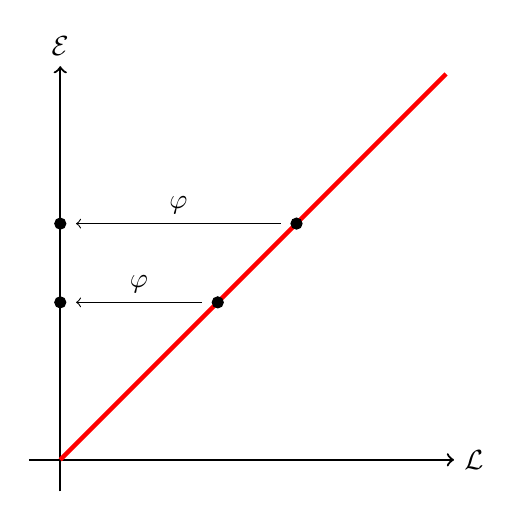
\begin{tikzpicture}
%\draw[help lines, color=gray!30, dashed] (-0.9,-0.9) grid (4.9,4.9);
\draw[->, thick] (-0.4,0)--(5,0) node[right]{$\mathcal{L}$};
\draw[->, thick] (0,-0.4)--(0,5) node[above]{$\mathcal{E}$};
\draw[-,ultra thick, red] (0,0)--(4.9,4.9);
\filldraw[black] (2,2) circle (2pt);
\filldraw[black] (0,2) circle (2pt);
\filldraw[black] (3,3) circle (2pt);
\filldraw[black] (0,3) circle (2pt);
\draw[->] (1.8,2) -- node[above] {$\varphi$} ++ (-1.6,0);
\draw[->] (2.8,3) -- node[above] {$\varphi$} ++ (-2.6,0);
\end{tikzpicture}
\end{subfigure}~
\begin{subfigure}[b]{0.49\textwidth}
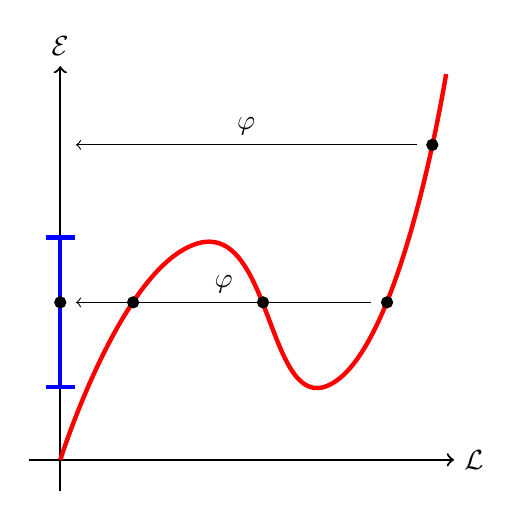
\begin{tikzpicture}
%\draw[help lines, color=gray!30, dashed] (-0.9,-0.9) grid (4.9,4.9);
\draw[->, thick] (-0.4,0)--(5,0) node[right]{$\mathcal{L}$};
\draw[->, thick] (0,-0.4)--(0,5) node[above]{$\mathcal{E}$};
\draw[|-|,ultra thick, blue] (0,0.9)--(0,2.85);
\draw [-, ultra thick, red] plot [smooth, tension=1] coordinates { (0,0) (1.75,2.75)  (3.5,1) (4.9,4.9)};
\filldraw[black] (0,2) circle (2pt);
\filldraw[black] (0.925,2) circle (2pt);
\filldraw[black] (2.575,2) circle (2pt);
\filldraw[black] (4.15,2) circle (2pt);
\filldraw[black] (4.725,4.) circle (2pt);
\draw[->] (3.95,2) -- node[above] {$\varphi$} ++ (-3.75,0);
\draw[->] (4.525,4.) -- node[above] {$\varphi$} ++ (-4.325,0);
\end{tikzpicture}
\end{subfigure}
\caption{Projection of phase-space to Eulerian space. The left panel illustrates the initial dark matter sheet in phase space. The arrow represents the projection to Eulerian space $\varphi$. The mapping is one-to-one. The right panel illustrates the dark matter sheet after it has evolved and formed a triple-stream region (in blue). Each point in the triple-stream region corresponds to three points on the dark matter sheet. The triple-stream region is bounded by a fold caustic at which matter shell crosses.}\label{fig:Phase-Space}
\end{figure}

Initially, the displacement field vanishes, $\bm{s}_0(\bm{q})=\bm{0}$, and the phase-space manifold is diagonal $M_0=\{(\bm{q},\bm{q})\,|\,\bm{q} \in \mathcal{L}\}$. The mapping $\varphi$ is one-to-one, corresponding to a single-stream region (see the left panel of figure\ \ref{fig:Phase-Space}). When the fluid evolves, the phase-space manifold can develop complex configurations at which the mapping $\varphi$ becomes many-to-one, \textit{i.e.}, a final position can be reached from multiple initial positions (see the right panel of figure \ref{fig:Phase-Space}). A connected region, in Eulerian space, with $n$ possible initial positions is known as an $n$-stream region. In these multi-stream regions, gravitational collapse becomes non-linear and viralized structures form. The multi-stream regions partition the universe into regions with distinct formation histories, based on the dynamics of gravitational collapse.  As we will show in the next section, different multi-stream regions can be associated to the membranes, filaments, and clusters of the cosmic web. The single-stream regions correspond to the voids, where the evolution of the cosmic web remains largely linear. See \cite{Hahn:2007, Abel:2012, Shandarin:2012,  Ramachandra:2015, Ramachandra:2017, Shandarin:2019, Shandarin:2021} for recent investigations into the phase-space structure of the cosmic web and the identification of multi-stream regions in $N$-body simulations.

The density of a Lagrangian fluid evolves while the mass elements are squeezed and stretched, \textit{i.e.},
\begin{align}
\rho_t(\bm{x})
&= \sum_{\bm{q} \in A_t(\bm{x})} \frac{\bar{\rho}}{|\det \nabla \bm{x}_t(\bm{q})|}\\
&= \sum_{\bm{q} \in A_t(\bm{x})} \frac{\bar{\rho}}{|1+\mu_{t,1}(\bm{q})||1+\mu_{t,2}(\bm{q})|}\,,
\label{eq:density}
\end{align}
with the mean initial density $\bar{\rho}$, and the eigenvalue fields $\mu_{t,1}$ and $\mu_{t,2}$ of the deformation tensor $\nabla \bm{s}_t$, defined by
\begin{align}
\nabla \bm{s}_t(\bm{q}) \bm{v}_{t,i}(\bm{q}) = \mu_{t,i}(\bm{q}) \bm{v}_{t,i}(\bm{q})\,.
\label{eq:EigenvalueAndEigenvector}
\end{align} 
Each stream contributes to the density, as the sum runs over the points that reach $\bm{x}$ in time $t$, \textit{i.e.},
\begin{align}
A_t(\bm{x}') = \{\bm{q}|\bm{x}_t(\bm{q})=\bm{x}'\}\,.
\end{align}
The boundaries of the multi-stream regions mark discontinuous of the density field \eqref{eq:density}. In fact, at the boundary, the orientation of the mass elements flip in a process known as \textit{shell-crossing}. The determinant $\det \nabla \bm{x}_t$ vanishes and the density spikes to infinity. This phenomenon is an example of a \textit{fold caustic}, bounding the regions where virialized structures emerge. In this paper, we always order the eigenvalue fields such that $\mu_{t,1}$ is the field which causes the first shell-crossing event. As we shall see in the next section, the -- often ignored -- eigenvector fields plays an important role in the higher order caustics.

\begin{figure}
\centering
\begin{subfigure}[b]{0.49\textwidth}
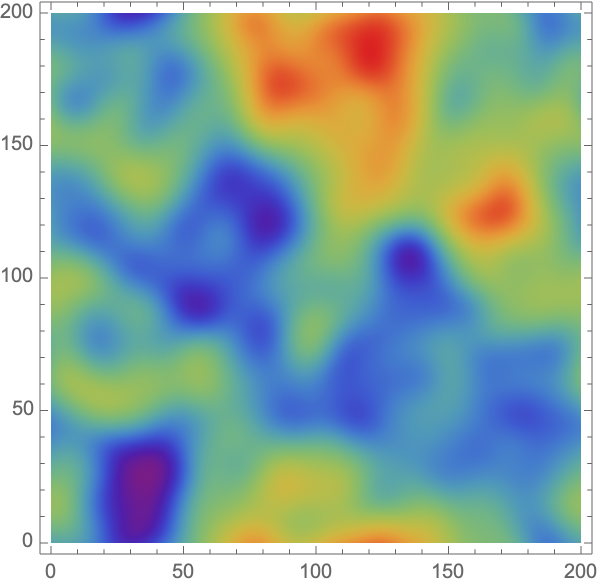
\includegraphics[width=\textwidth]{Psi}
\end{subfigure}~
\begin{subfigure}[b]{0.49\textwidth}
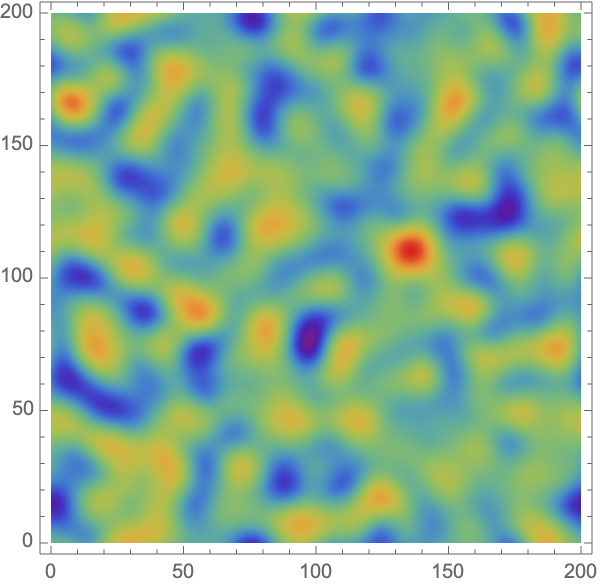
\includegraphics[width=\textwidth]{Rho}
\end{subfigure}\\
\begin{subfigure}[b]{0.49\textwidth}
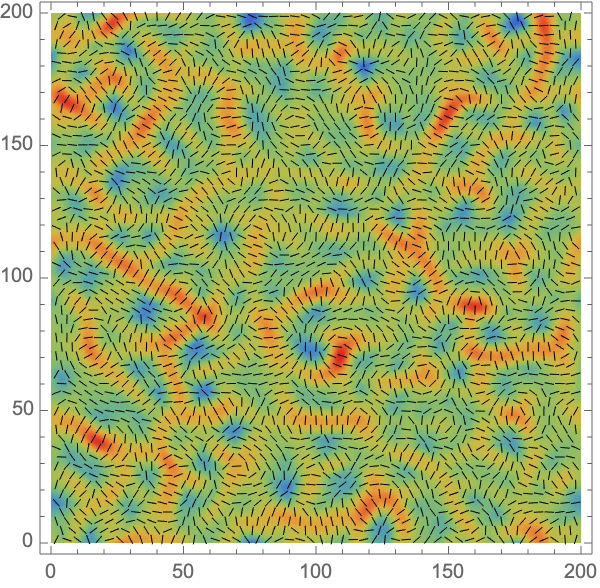
\includegraphics[width=\textwidth]{Lambda_1}
\end{subfigure}~
\begin{subfigure}[b]{0.49\textwidth}
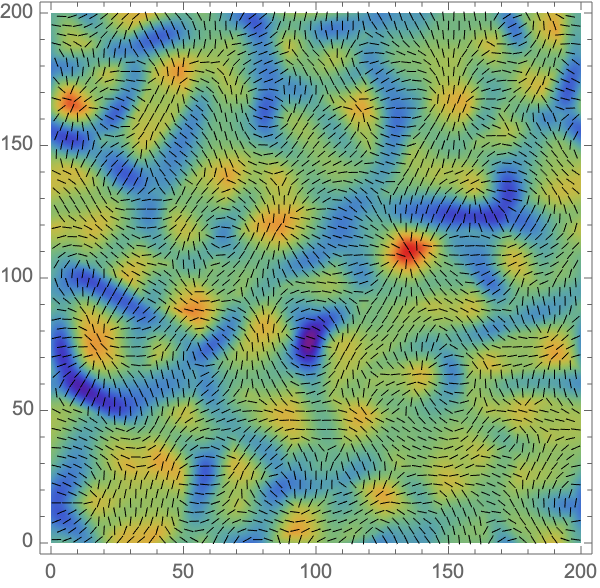
\includegraphics[width=\textwidth]{Lambda_2}
\end{subfigure}
\caption{A Gaussian random field and the corresponding eigenvalue and eigenvector fields. \textit{Upper left:} the gravitaitonal potential $\Psi$. \textit{Upper right:} the corresponding density perturbation field $\delta$. \textit{Lower left:} the first eigenvalue and eigenvector fields $\mu_1,\bm{v}_1$. \textit{Lower right:} the second eigenvalue and eigenvector fields $\mu_2,\bm{v}_2$.}\label{fig:Initial_Conditions}
\end{figure}

In late time cosmology, the cosmic web forms due to the gravitational collapse of tiny Gaussian fluctuations $\delta_0$. At early times, the corresponding Gaussian gravitational potential $\phi_0$ governs the dynamics of the mass elements, $\bm{s}_t \propto \nabla \phi_0$. See the upper panels of figure \ref{fig:Initial_Conditions} for an illustration of the initial density and the corresponding gravitational potential fields\footnote{We model the gravitational potential with a power-law power spectrum $P(k) \propto k^{n_s}$ with an index $n_s=-1$ smoothed with a Gaussian filter on the length scale $\sigma=5\text{ Mpc}$.}. Eulerian fluid dynamics describes the early evolution of the density field in terms of these Gaussian fields. In contrast, Lagrangian fluid dynamics emphasises the role of the deformation tensor $\nabla \bm{s}_t$ and the corresponding non-Gaussian eigenvalue and eigenvector fields (see the density formula \eqref{eq:density}). It follows from the eigenequation \eqref{eq:EigenvalueAndEigenvector} that the eigenvalue fields are the quadratic (or cubic) roots of a polynomial whose coefficients depend on the first order derivatives of the displacement field in 2D (or 3D). The non-linearity of the eigenvalue fields captures part of the non-linear dynamics of gravitational collapse. At early times the deformation tensor $\nabla \bm{s}_t$ is proportional to the Hessian of the gravitational potential, $\nabla \bm{s}_t \propto \mathcal{H}\phi_0$. The eigenvalue and eigenvector fields are nonlinear functions of the second order derivatives of the initial gravitational potential. See the lower panels of figure \ref{fig:Initial_Conditions} for an illustration of the non-Gaussian nature of the eigenvalue fields corresponding to the gravitational potential in the upper left panel. 

\begin{figure}
\centering
\begin{subfigure}[b]{0.45\textwidth}
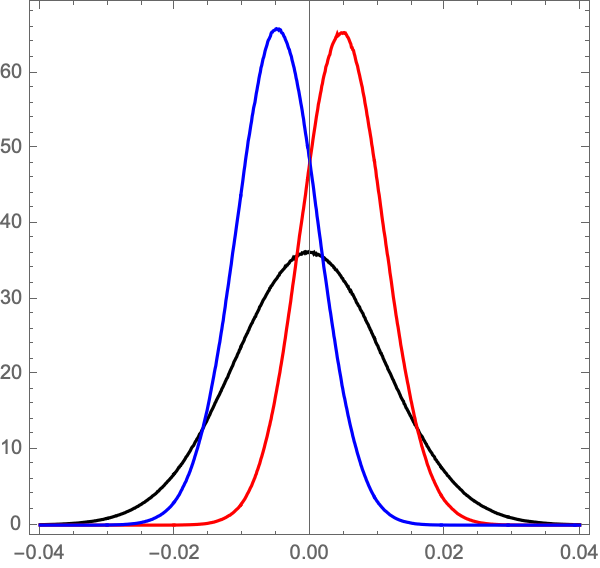
\includegraphics[width=\textwidth]{eigen_dens}
\end{subfigure}~
\begin{subfigure}[b]{0.45\textwidth}
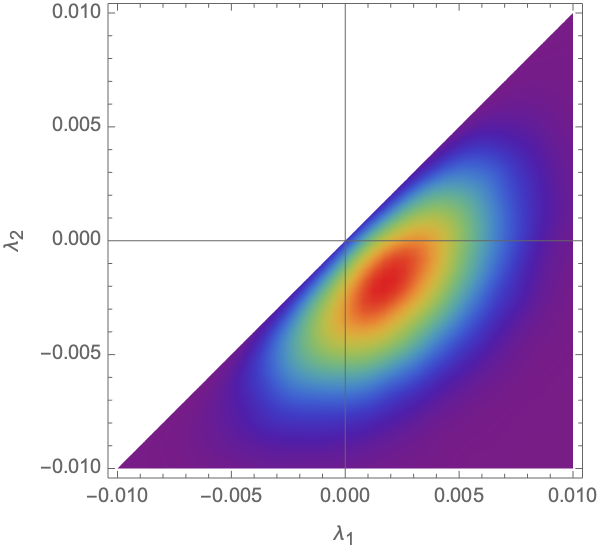
\includegraphics[width=\textwidth]{joint_eigen}
\end{subfigure}
\caption{The distirubtion of the eigenvalue fields. \textit{Left:} the PDF of the initial density perturbation $\delta$ (black) and the initial eigenvalue fields $\mu_{i,t}$ (red and blue). \textit{Right:} the joint distribution of the eigenvalue fields.}\label{fig:eigen_stats}
\end{figure}

The red regions experience an inflow of matter, leading to the first caustics. The blue regions represent an initial outflow of matter. Roughly speaking, the eigenvalue fields peak in the regions of high initial density. In particular, compare the peaks of the initial density field $\delta_0$ and the second eigenvalue field $\mu_{t,2}$. However, the density perturbation and the eigenvalue fields differ away from these high density regions. The eigenvalue fields emphasise line like features connecting the high density regions. As described below, these line-like features of the first eigenvalue field are the progenitors of the filaments of the cosmic web. 

It follows from the Poisson equation (see section \ref{sec:Zeldovich}), that the sum of the initial eigenvalue fields is proportional to the initial density perturbation, 
\begin{align}
\delta_0 \propto \nabla^2 \phi_0 = \text{Tr}[\mathcal{H}\phi_0] \propto \mu_{t,1} + \mu_{t,2}\,,
\end{align}
with the Hessian $\mathcal{H}$, demonstrating a non-trivial correlation between the initial eigenvalue fields. The eigenvalue fields splits the Gaussian initial density perturbations into parts which influence the linear regime of gravitational collapse in distinct ways. Moreover, the two initial eigenvalue fields are strongly correlated with the joint probability distribution given by the two-dimensional Doroshkevich formula \cite{Doroshkevich:1970, Feldbrugge:2014}
\begin{align}
p(\mu_1,\mu_2) = \frac{2\sqrt{2}}{\sqrt{\pi} \sigma_2^3} e^{-\frac{3(\mu_1+\mu_2)^2-8\mu_1 \mu_2}{2 \sigma_2^2}}|\mu_1-\mu_2|\,,
\end{align}
with $\sigma_2$ the generalized moment defined in section \ref{sec:GRF}. See figure \ref{fig:eigen_stats} for an illustration of the eigenvalue and density field statistics. 

As we will show, the orientation and geometry of the shell-crossing regions is further described by the eigenvector fields (see the lines in the lower panels of figure \ref{fig:Initial_Conditions}). At initial times, the eigenvector fields are normal, $\bm{v}_{t,1}\cdot \bm{v}_{t,2}=0$, since the deformation tensor is symmetric. Observe that the eigenvector fields exhibit an interesting correlation with the eigenvalue fields. Roughly speaking, the eigenvector fields are normal to the ridges of the corresponding eigenvalue fields. This observation will play an important role in the discussion of the caustic skeleton below. 


%%%%%%%%%%%%%%%%%%%%%%%%%%%%%%%%%%%%%%%%%%%%%%%%%%%%%%%%%%%%%%%%
\subsection{Caustics in Lagrangian fluids}
The study of the cosmic web in terms of multi-stream regions and Lagrangian catastrophe theory has a rich history, predating the developments of $N$-body simulations \cite{Arnold:1982a, Arnold:1982b, Shandarin:1983, Rozhanskii:1984, Shandarin:1989}. Amazingly, by analysing the geometry of the caustics emerging in Lagrangian fluid dynamics, Y.\ Zel'dovich, V.\ Arnol'd and collaborators successfully predicted the qualitative features of the cosmic web. However, these studies where mainly restricted to two-dimensional models, as several technical problems inhibited the full treatment of three-dimensional cosmic web. In a recent publication \cite{Feldbrugge:2018}, we solved these problems by formulating the \textit{shell-crossing condition} describing how a submanifold in $\mathcal{L}$ can develop a non-differentiable feature under the mapping $\bm{x}_t$. Given a submanifold $L \subset \mathcal{L}$, the mapping $\bm{x}_t(L)$ develops a non-differentiable point at time $t$ in $\bm{q}_c$ when there exists a non-zero vector tangent vector $\bm{T}$ in the tangent space of $L$ at $\bm{q}_c$ for which 
\begin{align}
(1+\mu_{t,i}(\bm{q}_c))\bm{v}_{t,i}^*(\bm{q}_c) \cdot \bm{T}=0
\label{eq:shellCrossingCondition}
\end{align}
for all $i$, with $\bm{v}_{i,t}^*$ the dual eigenvector field defined by the relation $\bm{v}_{t,i}\cdot \bm{v}_{t,j}^* = \delta_{ij}$.

The shell-crossing condition leads to a set of \textit{caustic conditions} describing the properties of the displacement field in the vicinity of a caustic. Remarkably, the caustic conditions demonstrate the key role of the eigenvalue $\mu_{t,i}$ and eigenvector fields $\bm{v}_{t,i}$ of the deformation tensor $\nabla \bm{s}_t$ over the density field in the development of viralized structures. The eigenvalue and eigenvector fields are non-linearly related to the gravitational potential and demonstrate how Gaussian initial conditions give rise to a web-like structure (see figure \ref{fig:Initial_Conditions}). As we show below, the geometry of the often 
ignored eigenvector fields (see for example \cite{Forero:2009}) is crucial to the development of the higher-order caustics, tracing the filaments and clusters of the cosmic web.

Lagrangian catastrophe theory classifies the shell-crossing regions into a finite set of caustics that stably occur in nature \cite{Arnold:1972, Arnold:1976, Poston:1978, Gilmore:1981, Kravtsov:1983, Arnold:1984, Arnold:2012a, Arnold:2012b}. These caustics have a direct connection to the walls, filaments and clusters of the cosmic web. The region for which the density spikes, \textit{i.e.}, 
\begin{align}
1+\mu_{t,i}(\bm{q}_c)=0
\end{align}
for $i=1$ or $2$, forms the fold curve $A_2$ consisting of the points that shell-cross at time $t$. Note that the fold curve is independent of the eigenvector fields and trivially satisfies the shell-crossing condition \eqref{eq:shellCrossingCondition}. The fold curve bounds the different multi-stream regions (see the red curves in figure \ref{fig:caustics_Examples_Big}). The analysis presented in figure \ref{fig:caustics_Examples_Big} is based on the caustic skeleton of the Zel'dovich approximation described below. However, the caustic conditions apply to general Lagrangian fluids. 

The initial gravitational potential in the examples in this paper are -- unless otherwise indicated -- based on a Gaussian random field with a power-law power spectrum $P(k) \propto k^{n_s}$ with the index $n_s=-1$ smoothed with a Gaussian filter with the length scale $\sigma = 5\text{ Mpc}$. We assume a flat Einstein-de Sitter universe consisting of dark matter density $\Omega_m=1$ with a Hubble constant $H_0=71\text{ km/s/Mpc}$. We map the caustic skeleton in Lagrangian space to Eulerian space with the Lagrangian map $\bm{x}_t$, where $\bm{x}_t$ either corresponds to the Zel'dovich approximation or a small dark matter two-dimensional $N$-body simulation \cite{Hidding:2020}.

The fold curve can develop a non-differentiable point in the cusp caustic $A_3$, when the fold curve in Lagrangian space is parallel to the corresponding eigenvector field, \textit{i.e.}, 
\begin{align}
1+\mu_{t,i}(\bm{q}_c)=0\,,\\
\bm{v}_{t,i}(\bm{q}_c) \cdot \nabla \mu_{t,i}(\bm{q}_c)=0\,,\label{eq:cuspCondition}
\end{align}
See the intersection of the red and blue curves in figure \ref{fig:caustics_Examples_Big}, where the tangent vector of the red line is parallel to the eigenvector field. The term $\bm{v}_{t,i} \cdot \nabla \mu_{t,i}$ arises in the shell-crossing condition \eqref{eq:shellCrossingCondition} from the observation that the tangent vector of the fold curve $\bm{T}$ is normal to the gradient of the eigenvalue field $\nabla \mu_{t,i}$. Over time, the cusp point defines the cusp curve which is associated to the filaments of the cosmic web. See the blue curve in the first row of figure \ref{fig:caustics_Examples_Big} for an example of a fold curve and its relation to the filaments of the cosmic web. 

In turn, the cusp curve develops a non-differentiable point known as a swallowtail caustic $A_4$ when the cusp curve in Lagrangian space is parallel to the eigenvector field, \textit{i.e.},
\begin{align}
1+\mu_{t,i}(\bm{q}_c)=0\,,\\
\bm{v}_{t,i}(\bm{q}_c) \cdot \nabla \mu_{t,i}(\bm{q}_c)=0\,,\\
\bm{v}_{t,i}(\bm{q}_c) \cdot \nabla (\bm{v}_{t,i}(\bm{q}_c) \cdot \nabla \mu_{t,i}(\bm{q}_c)) = 0\,.
\end{align}
The swallowtail caustic only exists for an instance and marks the location of a cluster, highlighting the location where different cusp curves join (see the second row of figure \ref{fig:caustics_Examples_Big}). 

In addition to the swallowtail caustic, the Lagrangian fluid also develops point-like caustics when both eigenvalue fields lead to a spike in the density field. The points for which
\begin{align}
1+\mu_{t,1}(\bm{q}_c) =0\,,\\
1+\mu_{t,2}(\bm{q}_c) = 0\,,
\end{align}
are known as the umbilic caustics $D_4^\pm$. The umbilic caustics consist of the elliptic $D_4^+$ and hyperbolic caustics $D_4^-$, both related to the clusters of the cosmic web. The umbilic caustics mark the locations where the cusp curves corresponding to the first and the second eigenvalue fields join (see the third and fourth rows of figure \ref{fig:caustics_Examples_Big}). 

Finally, caustic skeleton theory includes a set of Morse points, at which the multi-stream regions emerge, vanish and merge, changing the topology and connectivity of the cosmic web. The Morse points are defined as the critical points of the eigenvalue fields, satisfying the condition
\begin{align}
\nabla \mu_{t,i}(\bm{q}_c)=\bm{0}\,.
\end{align}
The maxima and minima of the eigenvalue field $\mu_i$ mark the locations and times at which a multi-stream region emerges or disappears. A critical point that undergoes shell-crossing always lies on a cusp curves, as a point with a vanishing gradient automatically satisfies equation \eqref{eq:cuspCondition}. The maxima and minima are known as $A_3^+$ points. The saddle point of the eigenvalue field $\mu_{t,i}$ mark the location and time at which two multi-stream regions merge to form a larger structure. At the $A_3^-$ point, two cusp curves corresponding to two filaments join. The Morse points determine the connectivity of the cosmic web. 

In tabel \ref{table:caustics}, we summarize the different elements of the caustic skeleton. For a complete contemporary description of caustic skeleton theory, we refer to \cite{Hidding:2014, Feldbrugge:2018}.\\


Note that the study of the Morse points of the caustic skeleton has a direct connection to the DisPerSE and the Felix classification schemes \cite{Pogosyan:2009, Sousbie:2011a, Sousbie:2011b, Shivashankar:2016}, which applies Morse-Smale theory to the density field. In this scheme, the critical points of the density field connect the maxima via integral lines, which are associated to the filaments of the cosmic web. However, the caustic skeleton differs from Morse-Smale theory in several respects. Firstly, in this paper, we focus on the deformation tensor instead of the density field. The eigenvalue fields tie into the dynamics of gravitational collapse. Secondly, the threshold of the the caustic skeleton is determined by the cosmic time (the growing mode for the Zel'dovich approximation). Finally, rather than connecting saddle points and maxima via integral lines satisfying a differential equation, the caustic skeleton connects the critical points using the simpler level sets \eqref{eq:cuspCondition}.


\begin{table}
\centering
{\scriptsize
\begin{tabular}{ |l | l | l | l | l|}
\hline
\textbf{Name} & \textbf{Symbol} & \textbf{2D cosmic web} & \textbf{Caustic conditions}\\
\hline
Fold & $A_2$ & shall-crossing & $1+ \mu_{t,i} = 0$ \\
\hline
Cusp & $A_3$ & filament & $1+ \mu_{t,i} = 0$, $\bm{v}_i \cdot \nabla \mu_{t,i} = 0$\\
\hline
Swallowtail &$A_4$ &  cluster & $1+ \mu_{t,i} = 0$, $\bm{v}_i \cdot \nabla \mu_{t,i} = 0,$ $\bm{v}_i \cdot \nabla(\bm{v}_i \cdot \nabla \mu_{i,t}) = 0$\\
\hline
Elliptic/hyperbolic & $D_4^{\pm}$ & cluster & $1+ \mu_{t,1} = 1+ \mu_{t,2} = 0$\\
\hline
Morse point & $A_3^+$ & creation/annihilation point& maximum/minimum of the eigenvalue field $\lambda_i$\\
\hline
Morse point & $A_3^-$ & merger point & saddle point of the eigenvalue field $\lambda_i$\\
\hline
\end{tabular}
}
\caption{Elements of the caustic skeleton.}
\label{table:caustics}
\end{table}


\begin{figure}
\centering
\begin{subfigure}[b]{0.3\textwidth}
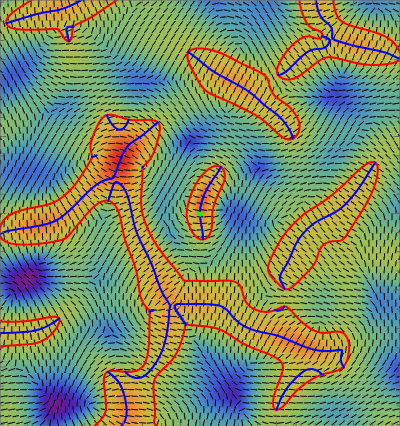
\includegraphics[width=\textwidth]{Cusp_L}
\end{subfigure}~
\begin{subfigure}[b]{0.3\textwidth}
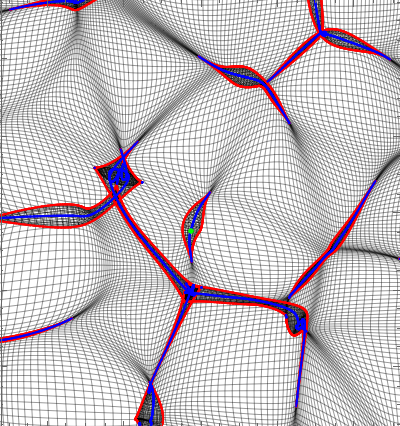
\includegraphics[width=\textwidth]{Cusp_Z}
\end{subfigure}~
\begin{subfigure}[b]{0.3\textwidth}
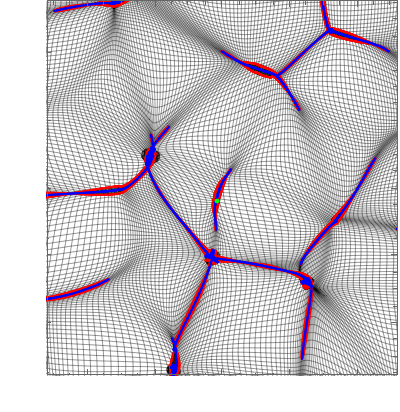
\includegraphics[width=\textwidth]{Cusp_Nb}
\end{subfigure}\\
%%%%%%%%%%
%%%%%%%%%%
\begin{subfigure}[b]{0.3\textwidth}
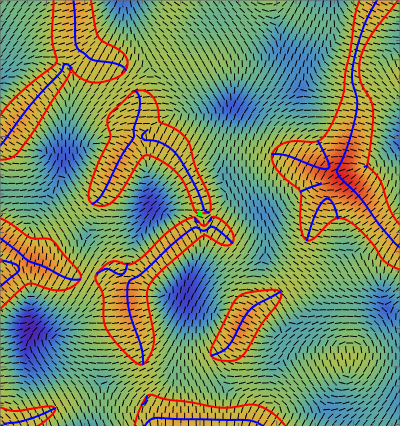
\includegraphics[width=\textwidth]{Swallowtail_L}
\end{subfigure}~
\begin{subfigure}[b]{0.3\textwidth}
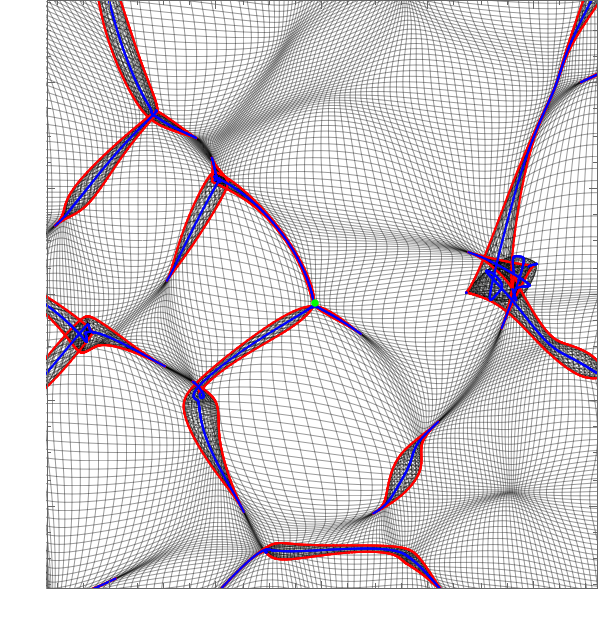
\includegraphics[width=\textwidth]{Swallowtail_Z}
\end{subfigure}~
\begin{subfigure}[b]{0.3\textwidth}
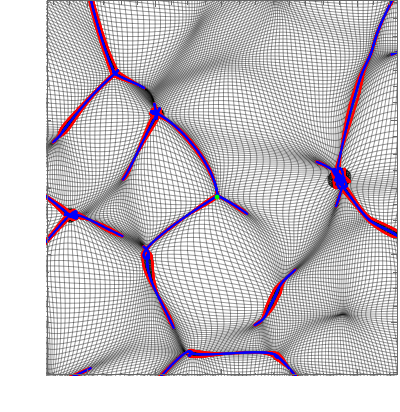
\includegraphics[width=\textwidth]{Swallowtail_Nb}
\end{subfigure}\\
%%%%%%%%%%
%%%%%%%%%%
\begin{subfigure}[b]{0.3\textwidth}
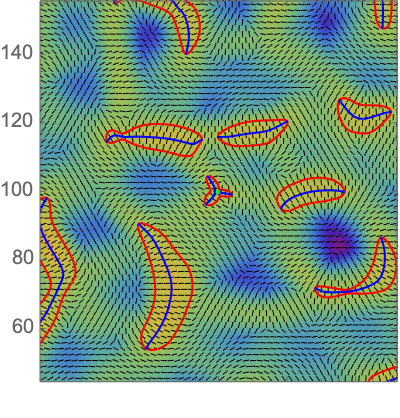
\includegraphics[width=\textwidth]{Elliptic_L}
\end{subfigure}~
\begin{subfigure}[b]{0.3\textwidth}
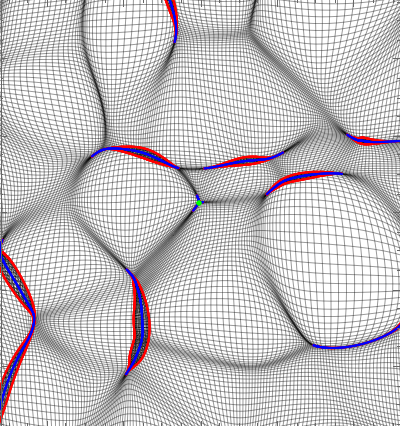
\includegraphics[width=\textwidth]{Elliptic_Z}
\end{subfigure}~
\begin{subfigure}[b]{0.3\textwidth}
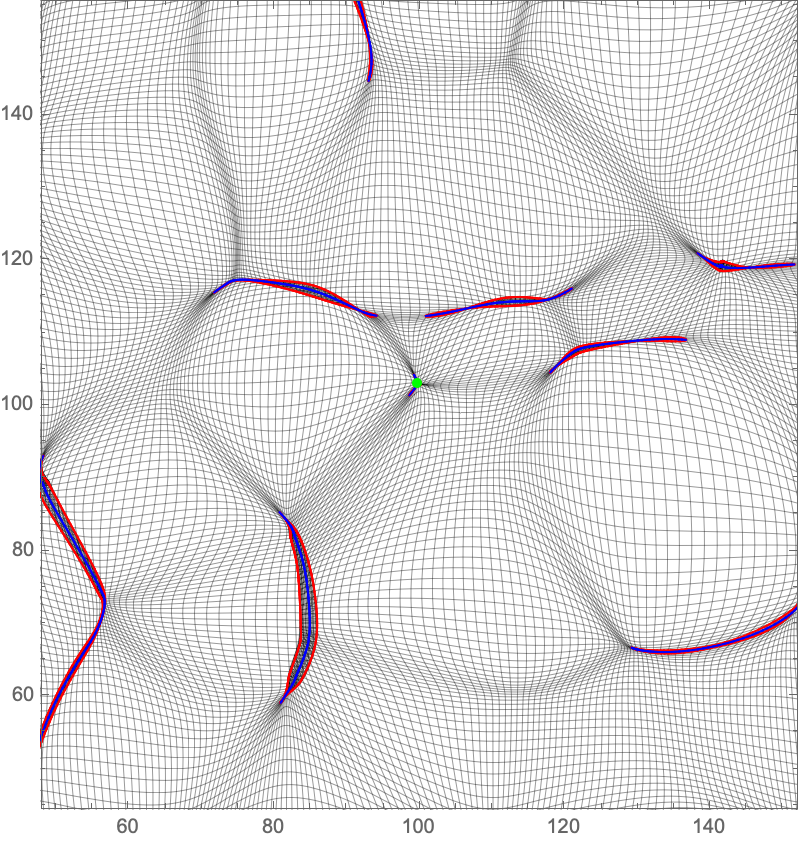
\includegraphics[width=\textwidth]{Elliptic_Nb}
\end{subfigure}\\
%%%%%%%%%%
%%%%%%%%%%
\begin{subfigure}[b]{0.3\textwidth}
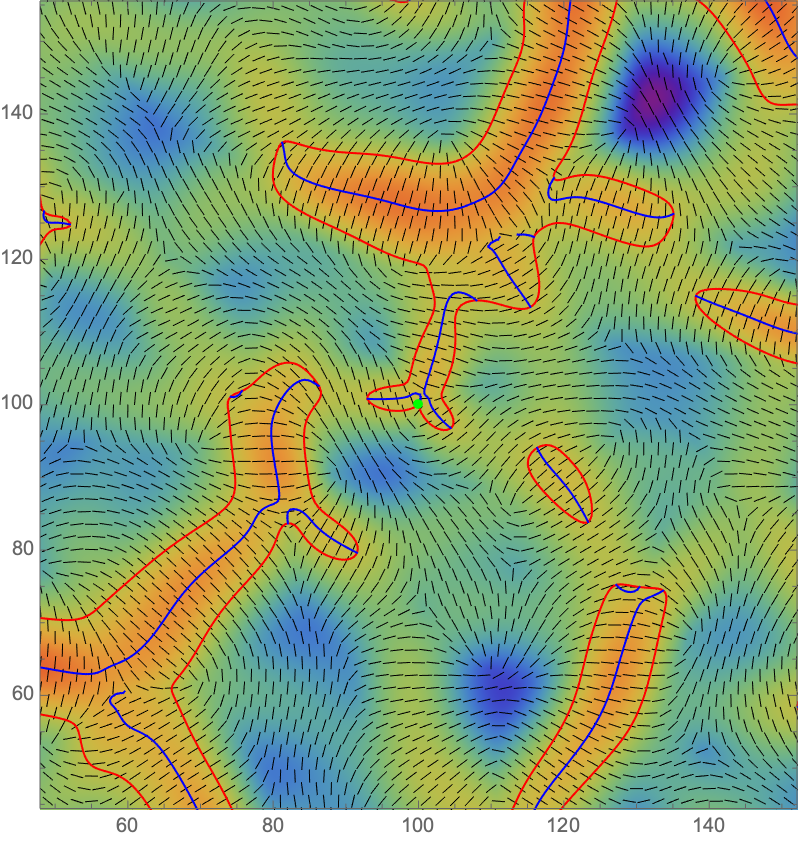
\includegraphics[width=\textwidth]{Hyperbolic_L}
\end{subfigure}~
\begin{subfigure}[b]{0.3\textwidth}
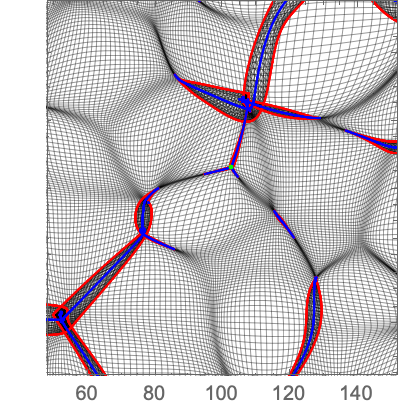
\includegraphics[width=\textwidth]{Hyperbolic_Z}
\end{subfigure}~
\begin{subfigure}[b]{0.3\textwidth}
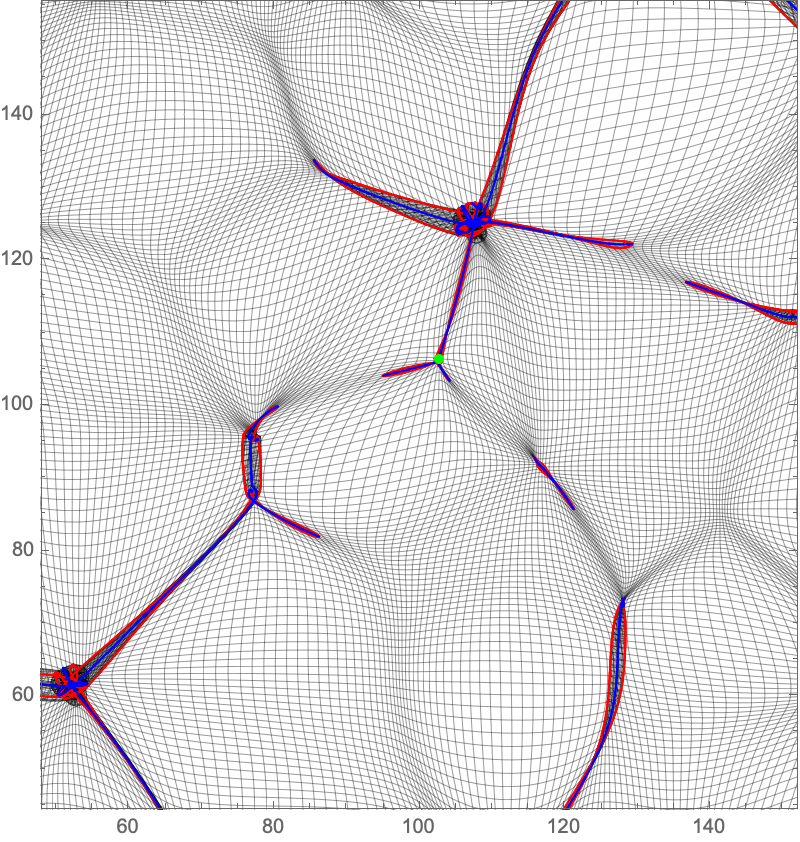
\includegraphics[width=\textwidth]{Hyperbolic_Nb}
\end{subfigure}
\caption{Elements of the caustic skeleton. \textit{From top to bottom:} the cusp, the swallowtail, the elliptic and the hyperbolic caustic. \textit{Left:} the caustic skeleton in Lagrangian space. \textit{Centre:} the Zel'dovich approximation. \textit{Right:} the corresponding $N$-body simulation \cite{Hidding:2020}.}\label{fig:caustics_Examples_Big}
\end{figure}

%%%%%%%%%%%%%%%%%%%%%%%%%%%%%%%%%%%%%%%%%%%%%%%%%%%%%%%%%%%%%%%%
\subsection{The Zel'dovich approximation}\label{sec:Zeldovich}
In this paper we define the caustic skeleton using the Zel'dovich approximation \cite{Zeldovich:1970} and study the resulting structures using a dark matter $N$-body simulation \cite{Hidding:2020}. The Zel'dovich approximation is the first order approximation in Lagrangian fluid dynamics, for which the displacement field factorizes into a spatial and a temporal part
\begin{align}
\bm{s}_t(\bm{q}) = - b_+(t) \nabla_{\bm{q}} \Psi(\bm{q})\,.
\end{align}
The growing mode $b_+(t)$ is a natural time parameter satisfying the differential equation
\begin{align}
\frac{\mathrm{d}^2 b_+(t)}{\mathrm{d}t^2} + 2 \frac{\dot{a}(t)}{a(t)} \frac{\mathrm{d} b_+(t)}{\mathrm{d}t} = 4 \pi G \rho_u(t) b_+(t)\,.
\end{align}
The displacement potential $\Psi$ captures the geometry of the cosmic web, and is proportional to the primordial gravitational potential
\begin{align}
\Psi(\bm{q}) &=\frac{1}{4 \pi G a^2 \rho_0}\phi_0(\bm{q})%\\
%&= \frac{2}{3\Omega_0 H_0^2}\phi_0(\bm{q})
\,,
\end{align}
expressed in terms of the current total energy density %$\Omega_0$ and
$\rho_0$,
%the current Hubble parameter $H_0$,
and the linearly extrapolated gravitational potential $\phi_0$. Note that the Poisson equation relates the primordial gravitational potential to the primordial density perturbation
\begin{align}
\nabla ^2 \phi_0 &= 4 \pi G a^2 \rho_u \delta_0\,.%\\
%&= \frac{3}{2} \Omega H^2 a^2 \delta\,,
\end{align}
In the Zel'dovich approximation, the mass elements follow linear trajectories that are completely determined by the primordial gravitational potential. The approximation accurately describes single-stream regions but fails when mass streams overlap and gravitational interactions between mass elements become important. When working with the Zel'dovich approximation, it is convenient to work in terms of the Hessian of the displacement potential,
\begin{align}
\bm{\psi}=\mathcal{H}\Psi\,,
\end{align}
and the corresponding eigenvalue $\lambda_i$ and $\bm{v}_i$
\begin{align}
\bm{\psi}\bm{v}_i = \lambda_i \bm{v}_i
\end{align}
with the relation $\lambda_1 =-\mu_2/b_+,\lambda_2 =-\mu_1/b_+$, assuming the ordering $\lambda_1(\bm{q}) \geq \lambda_2(\bm{q})$. In terms of the eigenvalue fields $\lambda_i$, the density takes the form 
\begin{align}
\rho_t(\bm{x})
&= \sum_{\bm{q} \in A_t(\bm{x})} \frac{\bar{\rho}}{|1-b_+(t) \lambda_1(\bm{q})||1-b_+(t) \lambda_2(\bm{q})|}\,.
\end{align}
Initially, the growing mode $b_+$ vanishes and the universe consists of a single-stream region. As the fluid collapses under self gravity, the growing mode $b_+$ increases. The fold caustics form at the level sets of the eigenvalue field $\{\bm{q}\,|\,\lambda_i(\bm{q})=1/b_+(t)\}$. From this picture we observe the direct connection between the critical points of the eigenvalue fields and the connectivity of the cosmic web.


%%%%%%%%%%%%%%%%%%%%%%%%%%%%%%%%%%%%%%%%%%%%%%%%%%%%%%%%%%%%%%%%
\subsection{Caustics in the cosmic web}

\begin{figure}
\centering
\begin{subfigure}[b]{0.24\textwidth}
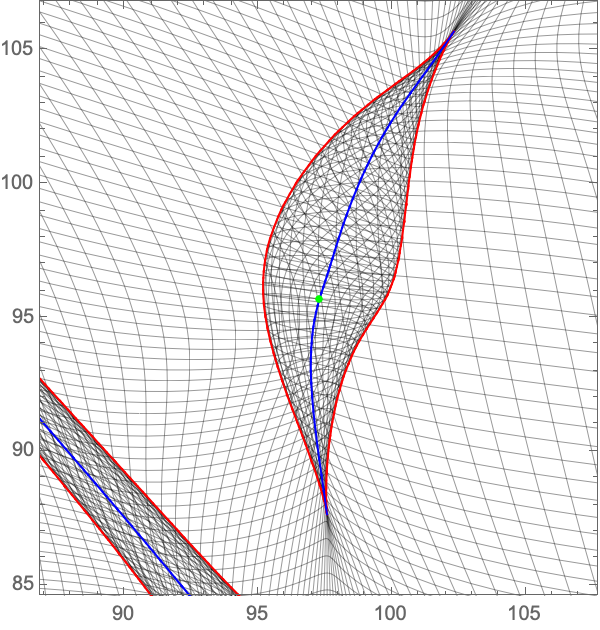
\includegraphics[width=\textwidth]{Cusp_Z_Zoom}
\end{subfigure}~
\begin{subfigure}[b]{0.24\textwidth}
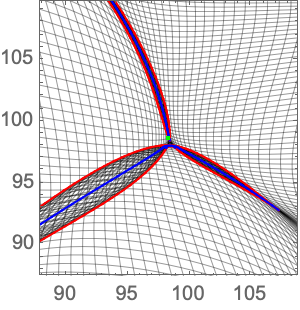
\includegraphics[width=\textwidth]{Swallowtail_Z_Zoom}
\end{subfigure}~
\begin{subfigure}[b]{0.24\textwidth}
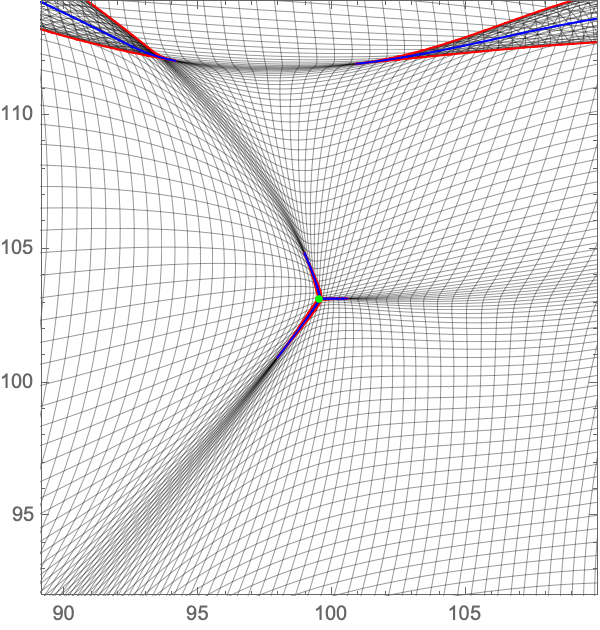
\includegraphics[width=\textwidth]{Elliptic_Z_Zoom}
\end{subfigure}~
\begin{subfigure}[b]{0.24\textwidth}
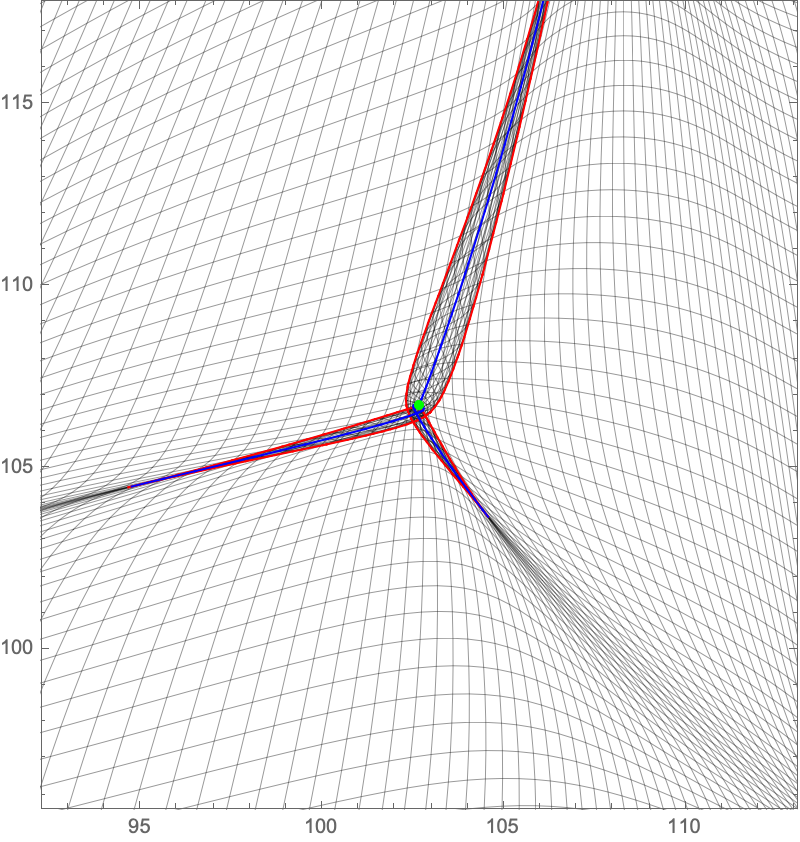
\includegraphics[width=\textwidth]{Hyperbolic_Z_Zoom}
\end{subfigure}\\
\begin{subfigure}[b]{0.24\textwidth}
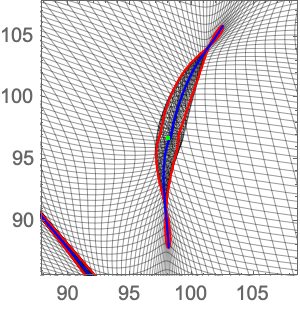
\includegraphics[width=\textwidth]{Cusp_Nb_Zoom}
\end{subfigure}~
\begin{subfigure}[b]{0.24\textwidth}
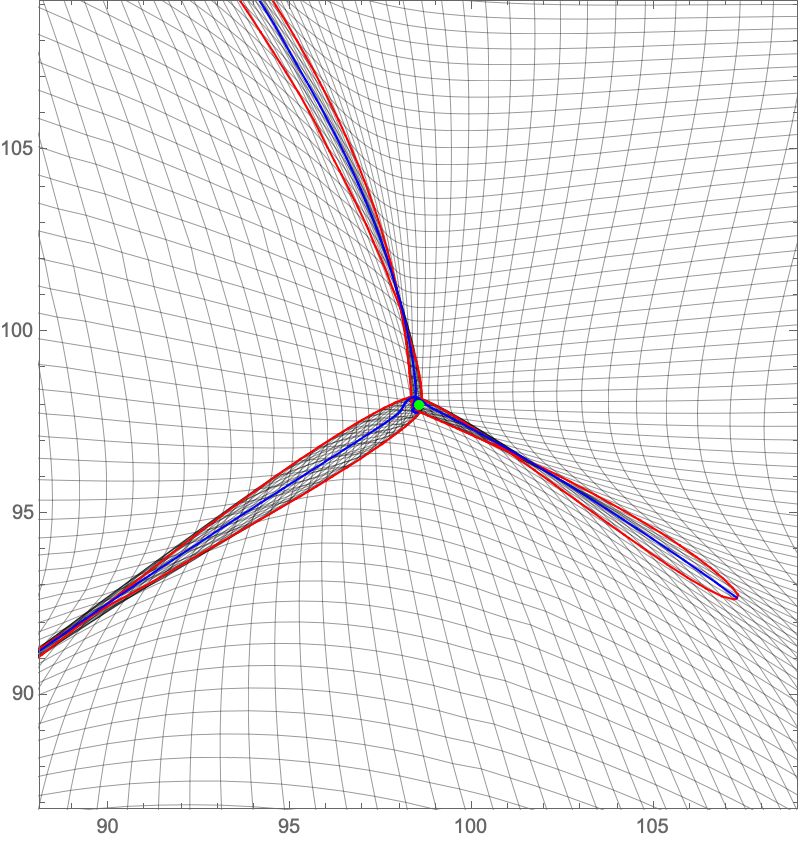
\includegraphics[width=\textwidth]{Swallowtail_Nb_Zoom}
\end{subfigure}~
\begin{subfigure}[b]{0.24\textwidth}
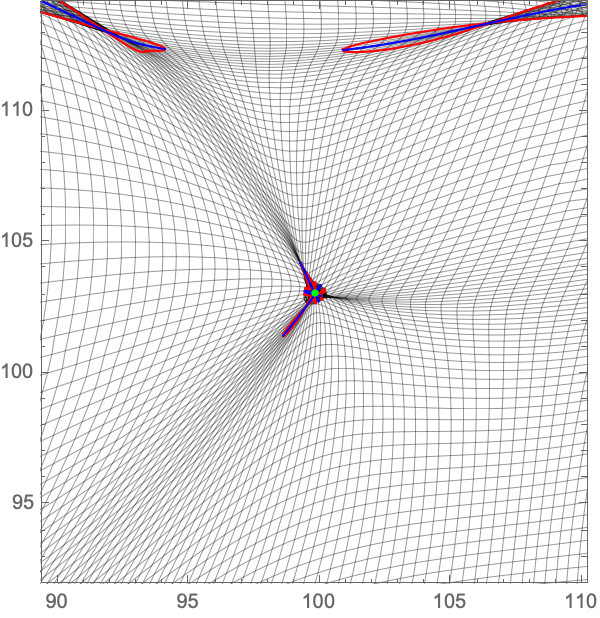
\includegraphics[width=\textwidth]{Elliptic_Nb_Zoom}
\end{subfigure}~
\begin{subfigure}[b]{0.24\textwidth}
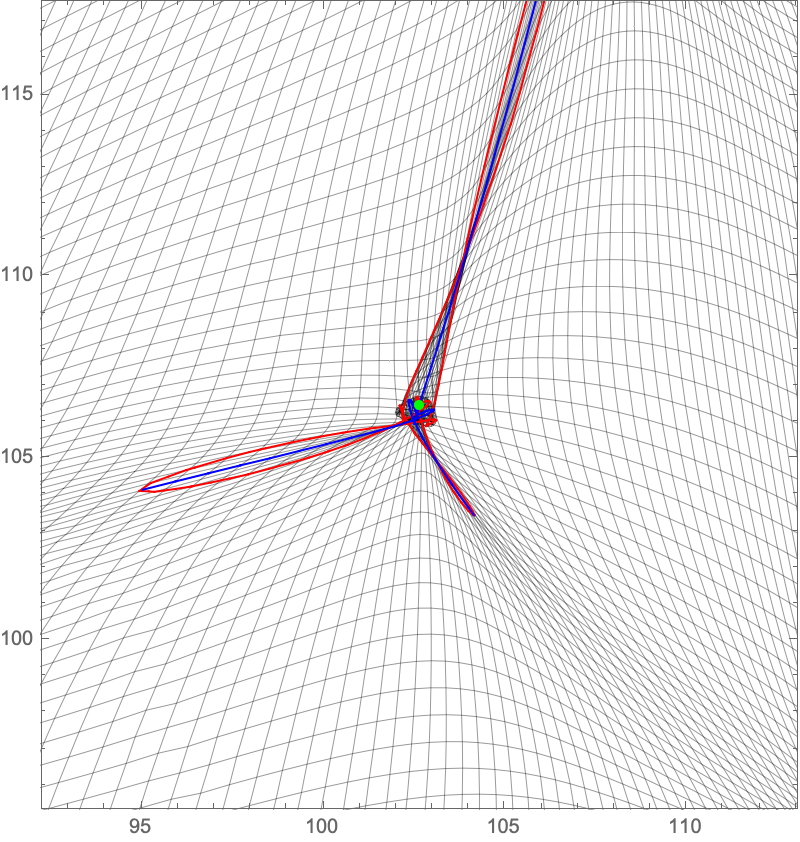
\includegraphics[width=\textwidth]{Hyperbolic_Nb_Zoom}
\end{subfigure}
\caption{Zoom in with a $(20 \text{ Mpc})^2$ box centred around the caustic. From left to right, we see the cusp, the swallowtail, the elliptic umbilic, and the hyperbolic umbilic caustics. The upper and lower panels display the Zel'dovich approximation and the $N$-body simulation \cite{Hidding:2020}.}\label{fig:caustics_Examples_Small}
\end{figure}


The role of the different elements of the caustic skeleton can be clearly observed from the zoom of figure \ref{fig:caustics_Examples_Big} centered on the caustic in Lagrangian space (see figure \ref{fig:caustics_Examples_Small}). The fold line is defined as the curve where the mass elements in the Zel'dovich approximation undergo shell-crossing. These shell-crossing regions clearly bound the multi-stream regions in the Zel'dovich approximation. This correspondence is less accurate in the $N$-body simulation, as the moment of shell-crossing may vary due to the non-linear nature of gravitational collapse. The cusp curve bisects the multi-stream region. The cusp curve marks the locations where the mass elements turn around to form a line-like structure. Note that this is valid in both the Zel'dovich approximation and the $N$-body simulation. The cusp curve in Lagrangian space accurately predict the mass elements around which matter virialized. The swallowtail, the elliptic and the hyperbolic caustics form where different cusp curves meet up to form a knot. The swallowtail caustic marks the place where the cusp curve corresponding to a single eigenvalue field becomes non-differentiable. The elliptic and hyperbolic caustics mark the location where the multi-stream regions of different eigenvalue fields merge. In figure \ref{fig:caustics_Examples_Small}, we observe that Zel'dovich approximation gives a good prediction of the geometry of the multi-stream regions in the $N$-body simulation at early times. Since the formation history of these different point caustics differs, it is natural to expect the properties of the different clusters to vary in nature. Note that the cluster caustics are rarely isolated. Caustics generally cluster and together form more intricate multi-stream structure. This way, a cluster can connect more than three filaments, even though the swallowtail, and umbilic caustics individually connect three filament regions.






%%%%%%%%%%%%%%%%%%%%%%%%%%%%%%%%%%%%%%%%%%%%%%%%%%%%%%%%%%%%%%%%
\section{Constrained random field theory}\label{sec:GRF}
One of the most startling realizations in modern cosmology is that the intricate cosmic web, observed in several cosmological redshift surveys, originated from extremely simple initial conditions. At the moment of recombination, when the baryons and electrons form neutral elements and decouple from the photons, the energy density in our universe $\rho(\bm{q})$, was extremely homogeneous. These fluctuations
\begin{align}
\delta(\bm{q}) = \frac{\rho(\bm{q})}{\bar{\rho}} -1\,,
\end{align}
with the mean density $\bar{\rho} = \langle \rho \rangle$ left an imprint as temperature fluctuations in the Cosmic Microwave Background field (CMB) which, over the last decades, have been measured with increasing accuracy \cite{WMAP:2003, Planck:2016}. After recombination, the pressure dropped and these density fluctuations started to collapse under the force of gravity. This led to the rich geometric patterns in the cosmic web and virialized objects we observe today. The statistical properties of these initial perturbations $\delta$, is very close to Gaussian \cite {Creminelli:2006, Planck:2020}. We here define Gaussian random fields and discuss the implementation of both linear and non-linear constraints. We closely follow the notation presented in \cite{Weygaert:1996}.

%%%%%%%%%%%%%%%%%%%%%%%%%%%%%%%%%%%%%%%%%%%%%%%%%%%%%%%%%%%%%%%%
\subsection{Gaussian random fields}
A two-dimensional Gaussian random field $f:\mathbb{R}^2\to \mathbb{R}$ is a continuous generalization of a multi-dimensional normal distribution, defined by the probability density
\begin{align}
p(\delta) = \mathcal{N} e^{- S[f]}\,, \label{eq:functional_Distribution}
\end{align}
with the normalization constant $\mathcal{N}$ and the `action' (in analogy with the Euclidean path integral \cite{Feynman:1965})
\begin{align}
S[f]\equiv \frac{1}{2} \iint (f(\bm{q}_1) - \bar{f}(\bm{q}_1)) K(\bm{q}_1,\bm{q}_2) (f(\bm{q}_2) -\bar{f}(\bm{q}_2))\mathrm{d}\bm{q}_1 \mathrm{d}\bm{q}_2,\label{eq:action}
\end{align}
defined in terms of the mean field $\bar{f}(\bm{q})$ and the kernel $K(\bm{q}_1,\bm{q}_2)$ \cite{Longuet-Higgins:1957, Adler:1981, bbks:1986}. The probability that the random field $f$ is included in a set of functions $\mathcal{S}$ is defined by the path integral
\begin{align}
P[f \in \mathcal{S}] = \mathcal{N} \int \bm{1}_\mathcal{S}(f) e^{-S[f]}\,\mathcal{D}f\,,
\end{align}
with $\bm{1}_\mathcal{S}$ the identity function\footnote{Defined by $\bm{1}_\mathcal{S}(x)=1$ when $x \in \mathcal{S}$ and $\bm{1}_\mathcal{S}(x)=0$ when $x \notin \mathcal{S}$.} and $\mathcal{D}f$ the path integral measure. The expectation value of a functional $Q[f]$ is given by
\begin{align}
\left\langle Q[f] \right\rangle = \mathcal{N}\int Q[f]\, e^{-S[f]}\,\mathcal{D}f\,,
\end{align}
analogous to the Euclidean path integrals in statistical field theory. It can be shown that the expectation value of the random field is given by the mean field
\begin{align}
\langle f(\bm{q})\rangle &= \bar{f}(\bm{q})\,.
\end{align}
Two-point correlation function
\begin{align}
\xi(\bm{q}_1, \bm{q}_2) &= \langle (f(\bm{q}_1) - \bar{f}(\bm{q}_1)) (f(\bm{q}_2) - \bar{f}(\bm{q}_2))\rangle\\
&= \int (f(\bm{q}_1) - \bar{f}(\bm{q}_1)) (f(\bm{q}_2) - \bar{f}(\bm{q}_2)) e^{-S[f]}\mathcal{D}f
\end{align}
is the inverse of the two-point correlation function,
\begin{align}
\int K(\bm{q}_1,\bm{q}) \xi(\bm{q},\bm{q}_2) \mathrm{d}\bm{q}= \delta_D^{(2)}(\bm{q}_1-\bm{q}_2)\,,\label{eq:defK}
\end{align}
with the two-dimensional Dirac delta function $\delta_D^{(2)}$. The Gaussian random field is thus fully determined by the mean field $\bar{f}$ and the two-point correlation function $\xi$. 

In cosmology, the cosmological principle often leads to the study of statistically homogeneous and isotropic random fields for which the mean field is constant $\bar{f}(\bm{q})=\bar{f}$ and the two point correlation function only depends on the magnitude of the difference of the inserted points, \textit{i.e.}, $\xi(\bm{q}_1,\bm{q}_2)=\xi(\|\bm{q}_1-\bm{q}_2\|)$, and consequently $K(\bm{q}_1,\bm{q}_2)=K(\|\bm{q}_1-\bm{q}_2\|)$. We will in particular consider random fields with vanishing means $\bar{f}=0$. 

The statistical properties of homogeneous and isotropic random fields are most transparently expressed in terms of the Fourier transformation of the random field
\begin{align}
\hat{f}(\bm{k}) = \int f(\bm{q})e^{i\bm{k}\cdot \bm{q}}\mathrm{d}\bm{q}\,,
\end{align}
and the inverse transform
\begin{align}
f(\bm{q}) = \int \hat{f}(\bm{k})e^{-i \bm{k} \cdot \bm{q}}\frac{\mathrm{d}\bm{k}}{(2\pi)^2}\,.
\end{align}
Note that the Fourier modes of real-valued Gaussian random fields satisfy the reality condition $\hat{f}(\bm{k}) = \hat{f}^*(-\bm{k})$. Using the double convolution theorem, we express the action \eqref{eq:action} as
\begin{align}
S[f] = \frac{1}{2} \int |\hat{f}(\bm{k})|^2 \hat{K}(\bm{k}) \frac{\mathrm{d}\bm{k}}{(2\pi)^2}\,.
\end{align}
In Fourier space, equation \eqref{eq:defK} takes the form
\begin{align}
\int \hat{K}(\bm{k})\, P(\bm{k})\, e^{i\bm{k}(\bm{q}_1-\bm{q}_2)} \frac{\mathrm{d}\bm{k}}{(2\pi)^2} = \delta_D^{(2)}(\bm{q}_1 - \bm{q}_2)\,,
\end{align}
with the power spectrum defined as the Fourier transform of the two-point correclation function,
\begin{align}
P(\bm{k}) = \int \xi(\bm{q}) \, e^{i\bm{k}\cdot \bm{q}}\mathrm{d}\bm{q}\,,
\end{align}
implying the relation $\hat{K}(\bm{k}) = 1/P(\|\bm{k}\|)$. The resulting probability density of the Fourier modes is diagonal
\begin{align}
p(\hat{f}) \propto \exp\left[ -\frac{1}{2} \int \frac{|\hat{f}(\bm{k})|^2}{P(\|\bm{k}\|)} \frac{\mathrm{d}\bm{k}}{(2\pi)^2}\right]\,,
\end{align}
implying the covariance
\begin{align}
\langle \hat{f}(\bm{k}_1)\hat{f}(\bm{k}_2) \rangle = (2\pi)^2 \delta_D^{(2)}(\bm{k}_1-\bm{k}_2) P(\|\bm{k}_1\|)\,.
\end{align}
In this paper, we for simplicity always assume the initial gravitational potential to be a realization of a homogeneous and isotropic Gaussian random field with a power-law power spectrum $P(k) \propto k^{n_s}$ smoothed with a Gaussian filter $W(k)=e^{-\sigma^2 k^2/2}$ with the spectral index $n_s$ and the smoothing scale $\sigma$. The effective power spectrum takes the form 
\begin{align}
P_{eff}(k)\propto k^{ns}e^{-\sigma^2 k^2}\,.
\end{align}
Unless otherwise specified, we use a spectral index $n_s=-1$ and a smoothing length scale $\sigma = 5\text{ Mpc}$. 



In practice, we often we often consider realizations of Gaussian random fields on a lattice, or more generally a finite set of linear statistics $\bm{Y}=(Y_1,Y_2,\dots,Y_M)$. In this setting, the functional distribution \eqref{eq:functional_Distribution} reduces to the multi-dimensional Gaussian distribution,
\begin{align}
p(\bm{Y}) = \frac{\exp\left[-\frac{1}{2} \sum_{i,j}^n \Delta \bm{Y}^T M^{-1} \Delta \bm{Y}\right]}{[(2\pi)^n \det M]^{1/2}}\,,
\end{align}
with the deviation from the mean $\Delta \bm{Y} = \bm{Y} - \langle \bm{Y}\rangle$ and the covariance matrix
\begin{align}
M = \text{cov}(\bm{Y},\bm{Y}) = \langle \Delta \bm{Y}^T \Delta \bm{Y}\rangle\,.
\end{align}
The distribution of the discrete Fourier modes $\bm{Y}(\hat{f}(\bm{k}_1),\hat{f}(\bm{k}_1),\dots)$ takes the form 
\begin{align}
p(\hat{f}(\bm{k}_1), \hat{f}(\bm{k}_2), \dots) = \prod_{i} \frac{1}{\sqrt{2\pi P(\| \bm{k}_i\|)}} e^{-\frac{|\hat{f}(\bm{k}_i)|^2}{2P(\|\bm{k}_i\|)}},
\end{align}
yielding an efficient method to generate realizations (see appendix \ref{ap:GRF}).

The statistical properties of random fields are often conveniently expressed in terms of the moments
\begin{align}
\sigma_i^2 &= \frac{1}{(2\pi)^2} \int \|\bm{k}\|^{2i}P(\|\bm{k}\|)\mathrm{d}\bm{k}\nonumber\\
&= \frac{1}{2\pi} \int_0^\infty k^{2i+1}P(k)\mathrm{d}k\,,
\end{align}
with the magnitude $k = \|\bm{k}\|$. The powerspectrum determines the covariance matrix $M$ through these moments. Whereas the variance of the random field is given by the moment $\sigma_0^2$, \textit{i.e.},
\begin{align}
\langle f(\bm{q})^2 \rangle &= \iint e^{i (\bm{p} - \bm{k})\cdot \bm{q}} \langle \hat{f}(\bm{k})\hat{f}^*(\bm{p})\rangle \frac{\mathrm{d}\bm{k}\mathrm{d}\bm{p}}{(2\pi)^4}\\
&=\frac{1}{(2\pi)^2}\int P(\|\bm{k}\|)\mathrm{d}\bm{k}=\sigma_0^2\,,
\end{align}
the expectation value of the square of the norm of the gradient takes the form
\begin{align}
\langle \|\nabla f(\bm{q})\|^2\rangle &= \langle \partial_1f(\bm{q})^2 + \partial_2 f(\bm{q})^2 \rangle \\
&= \iint [(ik_1)(-ip_1)+(ik_2)(-ip_2)] e^{i (\bm{p} - \bm{k})\cdot \bm{q}} \langle \hat{f}(\bm{k})\hat{f}^*(\bm{p})\rangle \frac{\mathrm{d}\bm{k}\mathrm{d}\bm{p}}{(2\pi)^4}\\
&=\frac{1}{(2\pi)^2}\int \|\bm{k}\|^2 P(\|\bm{k}\|)\mathrm{d}\bm{k}=\sigma_1^2\,,
\end{align}
with $\bm{k}=(k_1,k_2)$ and $\bm{p}=(p_1,p_2)$. By statistical isotropy, we obtain the variance of the first order partial derivatives
\begin{align}
\langle \partial_1 f(\bm{q})^2\rangle =\langle \partial_2 f(\bm{q})^2\rangle =\frac{\sigma_1^2}{2}\,.
\end{align}


%%%%%%%%%%%%%%%%%%%%%%%%%%%%%%%%%%%%%%%%%%%%%%%%%%%%%%%%%%%%%%%%
\subsection{Linear constraints: Gaussian fields}
In this paper, we study how the different geometric features of the cosmic web emerge from different initial conditions. To systematically study these initial conditions we use constrained Gaussian random field theory \cite{Bertschinger:1987, Hoffman:1991, Sheth:1995, Weygaert:1996}. In this section, we develop the theory of linear constraints following the analysis of \cite{Weygaert:1996}. In the next section, we generalize this discussion to a large class of non-linear constraints. We restrict both discussions to statistically homogeneous and isotropic fields with vanishing mean.

For a random field $f$, consider a set of linear constraints
\begin{align}
\Gamma =\{ C_i[f;\bm{q}_i] = c_i,\,\ i=1,\dots,M \}\,,
\end{align}
with the linear functional $C_i[f;\bm{q}]$ assuming the value $c_i$ in $\bm{q}_i$. A linear functional can take the form of the function value at a point
\begin{align}
C[f;\bm{q}'] &= f(\bm{q}')\,,
\end{align}
its derivative at a point
\begin{align}
C[f;\bm{q}'] &= \frac{\partial}{\partial q_i}f(\bm{q}')\,,
\end{align}
or more generally a convolution
\begin{align}
C[f;\bm{q}'] &= \int g(\bm{q}' - \bm{q})f(\bm{q})\mathrm{d}\bm{q}\,,
\end{align}
with the convolution kernel $g$. 

The constraint random field follows the distribution
\begin{align}
p(f|\Gamma) = \frac{p(f,\Gamma)}{p(\Gamma)}\,,
\end{align}
where the constraints follow the Gaussian marginal distribution
\begin{align}
p(\Gamma) = \frac{\exp\left[-\frac{1}{2} \Delta\bm{C}^T Q^{-1} \Delta\bm{C} \right]}{[(2\pi)^M \det Q]^{1/2}}\,,
\end{align}
with the vector $\bm{C}=(C_1[f;\bm{q}_1], \dots, C_M[f;\bm{q}_M])$ and the covariance matrix $Q = \text{cov}(\bm{C}, \bm{C})$. We can write the constraint distribution as the Gaussian probability density
\begin{align}
p(f|\Gamma) \propto  e^{-\frac{1}{2} \left[\iint f(\bm{q}_1) K(\|\bm{q}_1 - \bm{q}_2\|) f(\bm{q}_2)\mathrm{d}\bm{q}_1 \mathrm{d}\bm{q}_2 -\Delta \bm{C}^TQ^{-1}\Delta \bm{C}\right]},\label{eq:constraint1}
\end{align}
in the space of functions satisfying the constraints $\Gamma$. In appendix \ref{ap:constraintDensity}, we derive the mean field
\begin{align}
\bar{f}_{\bm{c}}(\bm{q})&=\langle f(\bm{q})|\Gamma\rangle \\
&= \bar{f}(\bm{q}) + \sum_{i,j=1}^M\xi_i (\bm{q})\xi_{ij}^{-1}(c_j-\bar{C}_j)\,,
\end{align}
and the covariance
\begin{align}
\text{cov}(f(\bm{q}_1),f(\bm{q}_2)|\Gamma)  = \xi(\bm{q}_1,\bm{q}_2) - \sum_{i,j=1}^M\xi_i(\bm{q}_1)\xi_{ij}^{-1}\xi_j(\bm{q}_2)\,,
\end{align}
with the covariance of the random field and the constraints $\xi_{i}(\bm{q}) = \text{cov}( f(\bm{q}), C_i)$ and the covariance matrix of the constraints $\xi_{ij} = \text{cov}( C_i ,C_j)$. Note that the covariance is independent of the value $\bm{c}$ the constraint $\bm{C}$ assumes. This is a special property of Gaussian distributions and linear constraints. Consequently, the probability density takes the form
\begin{align}
p( f|\Gamma) \propto  e^{-\frac{1}{2} \iint \delta{f}(\bm{q}_1) \tilde{K}(\bm{q}_1,\bm{q}_2) \delta f(\bm{q}_2)\mathrm{d}\bm{q}_1 \mathrm{d}\bm{q}_2 }\,,\label{eq:constraint2}
\end{align}
with the residue $\delta f = f-\langle f(\bm{q})|\Gamma\rangle$ and the constrained kernel $\tilde{K}$ defined as the inverse of the constrained two-point correlation function, \textit{i.e.},
\begin{align}
\int \tilde{K}(\bm{q}_1,\bm{q}) \left[\xi(\bm{q},\bm{q}_2) - \sum_{i,j=1}^M\xi_i(\bm{q})\xi_{ij}^{-1}\xi_j(\bm{q}_2)\right]\mathrm{d}\bm{q}= \delta_D^{(2)}(\bm{q}_1-\bm{q}_2)\,.
\end{align}
Note that earlier papers \cite{Bertschinger:1987, Hoffman:1991, Sheth:1995, Weygaert:1996} worked in the space of functions satisfying the constraints $\Gamma$, neglecting the correction $\sum_{i,j=1}^M\xi_i(\bm{q})\xi_{ij}^{-1}\xi_j(\bm{q}_2)$, and using the original kernel $K$ for the residue. In this study, we prefer to work in space of unrestricted functions, as the correction makes the inhomogeneity and anisotropy of the residue manifest. These properties are most clearly observed in the variance of the residue,
\begin{align}
\langle \delta f(\bm{q})^2|\Gamma \rangle = \sigma_0^2- \sum_{i,j=1}^M\xi_i(\bm{q})\xi_{ij}^{-1}\xi_j(\bm{q})\,,
\end{align}
which vanishes on the constraints. Away from the constraints, the variance of the residue approaches the variance of the unconstrained  field $\text{var}(f)=\sigma_0^2$.

The Hoffman-Ribak method cleverly uses the property that the statistics of the residue $\delta f$ are independent of $\bm{c}$, to generate realizations of the constraint Gaussian random field \cite{Hoffman:1991, Weygaert:1996}. Firstly, generate a realization $g$ of the unconstraint Gaussian random field with the required power spectrum. Secondly, evaluate the constraints for this realization $C_i[g;\bm{q}'_i]=d_i$ and the corresponding mean field $\bar{g}$. The statistical properties of the residue with respect to this mean field $\delta g = g-\bar{g}$ are independent of the value the constraints assume and thus identical to the properties of the residue $\delta f$. We can thus identify the residue $\delta g$ of the field $g$ with the residue $\delta f$ of the constrained field $f$. By adding the residue of the unconstraint field to the mean field with the required constraints, we obtain the realization of the constrained Gaussian random field. For more details see appendix \ref{ap:GRF}.

To judge the relevance of a particular set of constraints, it is useful to evaluate the $\chi^2$ of the set of values $c_i$,
\begin{align}
\chi^2 = \sum_{i,j=1}^M (c_i-\bar{C}_i)\, \xi_{ij}^{-1}(c_j-\bar{C}_j)\,,
\end{align}
which follows the chi-squared distribution with $M$ degrees of freedom. This is the Mahalanobis distance. The probability that one obtains a $\chi^2$ higher than this value in an unconstrained Gaussian random field, with the same power spectrum, is given by $\Gamma\left(\frac{M}{2}, \frac{\chi^2}{2}\right)/\Gamma\left(\frac{M}{2}\right)$, with the gamma function $\Gamma(x)$ and the upper incomoplete gamma function $\Gamma(s,x)$.

%%%%%%%%%%%%%%%%%%%%%%%%%%%%%%%%%%%%%%%%%%%%%%%%%%%%%%%%%%%%%%%%
\subsection{Non-linear constraints: formalism}
For the systematic investigation of the caustic skeleton, we extend constraint Gaussian random field theory to include non-linear constraints. More specifically, we extend the theory of linear constraints to the large class of non-linear constraints expressed in terms of a finite number of linear statistics.

Consider the set of linear functionals $C_i[f,\bm{q}_i]$ with $i=1,\dots,M$ and the space of values $\bm{c}=(c_1,\dots,c_M)$ the linear functionals can assume $\mathbb{R}^M$. On this space, we define a set of functions $\mathcal{C}_i:\mathbb{R}^M \to \mathbb{R}$ with $i=1,\dots,N$ and $N\leq M$, and the non-linear constraint $\Gamma = \{\mathcal{C}_i(\bm{C}) = 0\}_{i=1}^N$. We can visualize this geometrically by considering the $(M-N)$-dimensional constraint manifold $\mathcal{M}_\mathcal{C}$ in the space of the $M$ linear constraints
\begin{align}
\mathcal{M}_{\mathcal{C}} = 
\{\bm{c}\, |\, \mathcal{C}_i(\bm{c}) = 0 \text{ for all } i=1,\dots,N\}.
\end{align}
See figure \ref{fig:constraintManifold} for a sketch of this constraint manifold. On the manifold $\mathcal{M}_\mathcal{C}$, the constraint probability density is proportional to the original Gaussian distribution
\begin{framed}
\begin{align}
p(\bm{c}\,|\,\bm{c}\in \mathcal{M}_{\mathcal{C}})  = \frac{p(\bm{c})}{\int_{\mathcal{M}_\mathcal{C}} p(\bm{c})\, \mathrm{d}\bm{c}}\,.
\end{align}
\end{framed}
Note that the curvature of $\mathcal{M}_\mathcal{C}$ generally makes the induced density $p(\bm{c}\,|\,\bm{c}\in \mathcal{M}_{\mathcal{C}})$ non-Gaussian. We extend constraint Gaussian random field theory to include non-linear constraints by studying the finite dimensional probability density $p(\bm{c}\,|\,\bm{c}\in \mathcal{M}_{\mathcal{C}})$:



\begin{figure}
\centering
\begin{subfigure}[b]{0.49\textwidth}
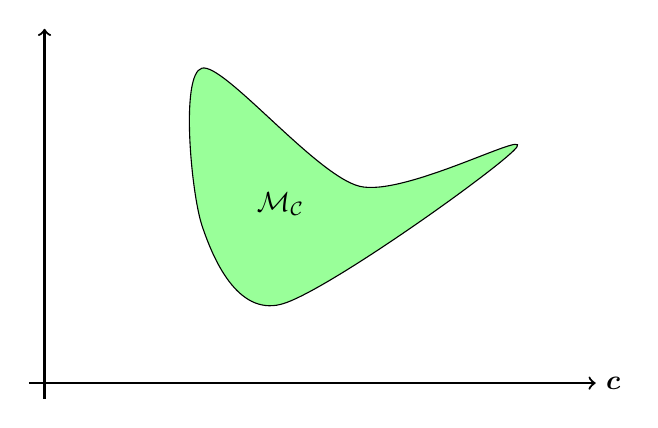
\begin{tikzpicture}
%\draw[draw=black] (0,0) rectangle ++(7,5);
\draw[->, thick] (-0.2,0)--(7,0) node[right]{$\bm{c}$};
\draw[->, thick] (0,-0.2)--(0,4.5);
%\draw [fill=blue!80] plot [mark=none, smooth cycle] coordinates {(2,2) (3,1) (6,3) (4,2.5) (2,4)};
\draw [fill=green!40] plot [mark=none, smooth cycle] coordinates {(2,2) (3,1) (6,3) (4,2.5) (2,4)};
%\draw [fill=lime!70] plot [mark=none, smooth cycle] coordinates {(2,2) (3,1) (6,3) (4,2.5) (2,4)};
\node[above] at (3,2) {$\mathcal{M}_\mathcal{C}$};
\end{tikzpicture}
\end{subfigure}
\caption{The constraint manifold $\mathcal{M}_\mathcal{C}$ in the space of linear constraint values.}\label{fig:constraintManifold}
\end{figure}


\begin{itemize}
\item
The problem of generating realizations of the more general constraints fields is reduced to sampling realizations of the distribution $p(\bm{c}|\bm{c}\in \mathcal{M}_\mathcal{C})$. Given a sample $\bm{c}$, we use the Hoffman-Ribak method to generate the realization.

\item
The mean field of the constrained field assumes the surprisingly suggestive form 
\begin{framed}
\begin{align}
\bar{f}_{\mathcal{C}}(\bm{q}) =\bar{f}_{\bar{\bm{c}}}(\bm{q})\,,
\end{align}
\end{framed}
with the mean constraint
\begin{align}
\bar{\bm{c}} &\equiv \langle \bm{c} \,|\, \Gamma\rangle = \int_{\bm{c} \in \mathcal{M}_{\mathcal{C}}}  \bm{c}\, p(\bm{c}\,|\,\bm{c}\in \mathcal{M}_{\mathcal{C}}) \mathrm{d}\bm{c}\,,
\end{align}
following from the realization  
\begin{align}
\bar{f}_{\mathcal{C}}(\bm{q}) 
&=\left\langle f(\bm{q})|\Gamma\right \rangle \nonumber\\
&= \int_{\bm{c} \in \mathcal{M}_{\mathcal{C}}} \bar{f}_{\bm{c}}(\bm{q})\, p(\bm{c}|\bm{c}\in \mathcal{M}_{\mathcal{C}}) \mathrm{d}\bm{c}\nonumber\\
&= \sum_{i,j=1}^n\xi_i(\bm{q}) \xi_{ij}^{-1}\int_{\bm{c} \in \mathcal{M}_{\mathcal{C}}}  (c_j-\bar{C}_j)\, p(\bm{c}|\bm{c}\in \mathcal{M}_{\mathcal{C}}) \mathrm{d}\bm{c}\nonumber\\
&= \sum_{i,j=1}^n \xi_i(\bm{q}) \xi_{ij}^{-1} (\bar{c}_j-\bar{C}_j)\nonumber\\
&= \bar{f}_{\bar{\bm{c}}}(\bm{q})\,.
\end{align}

\item
The residue $\delta f = f - \bar{f}_{\mathcal{C}}$ is generically no longer a Gaussian random field. The variance of the residue yields
\begin{framed}
\begin{align}
\left \langle \delta f (\bm{q})^2\,|\,\Gamma\right\rangle =
\sigma_0^2 - \sum_{i,j=1}^M\xi_i(\bm{q}) \xi_{ij}^{-1} \xi_j(\bm{q}) + \sum_{i,j,k,l=1}^M \xi_{i}(\bm{q})\xi_{ij}^{-1}\xi_{k}(\bm{q})\xi_{kl}^{-1}\text{cov}(c_j, c_l|\bm{c}\in\mathcal{M}_\mathcal{C})
\,,
\end{align}
\end{framed}
where $\text{cov}(c_j, c_l|\bm{c}\in\mathcal{M}_\mathcal{C})$ captures the geometry of the constraint manifold $\mathcal{M}_\mathcal{C}$, following directly from
\begin{align}
\left \langle \delta f (\bm{q})^2\,|\,\Gamma\right\rangle 
&= \int_{\mathcal{M}_\mathcal{C}} \langle (f(\bm{q})-\bar{f}_{\bar{\bm{c}}}(\bm{q}))^2|C_i[f,\bm{q}_i]=c_i\rangle p(\bm{c}|\bm{c}\in\mathcal{M}_{\mathcal{C}})\mathrm{d}\bm{c}\\
&= \int_{\mathcal{M}_\mathcal{C}} \langle f^2(\bm{q})|C_i[f,\bm{q}_i]=c_i\rangle p(\bm{c}|\bm{c}\in\mathcal{M}_{\mathcal{C}})\mathrm{d}\bm{c} - \bar{f}_{\bar{\bm{c}}}^2(\bm{q})\\
&= \int_{\mathcal{M}_\mathcal{C}} \langle (f(\bm{q})-\bar{f}_{\bm{c}}(\bm{q}))^2|C_i[f,\bm{q}_i]=c_i\rangle p(\bm{c}|\bm{c}\in\mathcal{M}_{\mathcal{C}})\mathrm{d}\bm{c} \\
&\ \ +\int_{\mathcal{M}_\mathcal{C}} (\bar{f}_{\bm{c}}(\bm{q})- \bar{f}_{\bar{\bm{c}}}^2(\bm{q}))^2p(\bm{c}|\bm{c}\in\mathcal{M}_{\mathcal{C}})\mathrm{d}\bm{c} \\
&=  \sigma_0^2 - \sum_{i,j=1}^M\xi_i(\bm{q}) \xi_{ij}^{-1} \xi_j(\bm{q}) + \sum_{i,j,k,l=1}^M \xi_{i}(\bm{q})\xi_{ij}^{-1}\xi_{k}(\bm{q})\xi_{kl}^{-1}\text{cov}(c_j, c_l|\bm{c}\in\mathcal{M}_\mathcal{C})\,.
\end{align}
Note that the variance of the residue with respect to the non-linear constraint is no longer independent of the values the constraint assumes. When $\mathcal{M}_\mathcal{C}$ consists of a point, the variance reduces to the linear case.
\end{itemize}



%%%%%%%%%%%%%%%%%%%%%%%%%%%%%%%%%%%%%%%%%%%%%%%%%%%%%%%%%%%%%%%%
\subsection{Non-linear constraints: case study}
A good example of a non-linear constraint is the requirement that the gradient of the Gaussian random field has a unit norm $\|\nabla f(\bm{q}_c)\|=1$. For this condition, we consider the space of first order derivatives
\begin{align}
\bm{C}=(\partial_x f, \partial_y f)\,,
\end{align}
and the non-linear constraint 
\begin{align}
\mathcal{C}(\bm{C})=\partial_x f^2 +  \partial_y f^2 - 1=0\,.
\end{align}
The constraint manifold $\mathcal{M}_\mathcal{C}=\{(\partial_xf,\partial_yf)\, |\, \partial_xf^2+\partial_yf^2=1\}$ is the unit circle in the space of first order derivatives (see figure \ref{fig:constraintManifold}).

For a statistically isotropic Gaussian random field, the constrained probability density is uniform $p(\bm{c}\, |\, \bm{c}\in\mathcal{M}_\mathcal{C}) = 1/(2\pi)$. After sampling from the constraint manifold, we construct a corresponding realization using linear constrained Gaussian random field theory. Both the mean and the covariance of the constraint value with respect to the constraint manifold vanish.

When the Gaussian random field is not statistically isotropic, the constraint density $p(\bm{c}\, |\, \bm{c}\in\mathcal{M}_\mathcal{C})$ is no longer uniformly distributed. We can construct realizations of the constrained Gaussian random field using rejection sampling on the constraint manifold. First, determine the maximum $max$ of $p(\bm{c})$ restricted to $\mathcal{M}_\mathcal{C}$. Secondly, generate a uniformly sampled point $\bm{c}$ on the unit circle $\mathcal{M}_\mathcal{C}$. Finally, we accept this sample $\bm{c}$ with probability $p(\bm{c})/max$. Once we have sampled the points on the constraint manifold $\mathcal{M}_\mathcal{C}$, we again construct a corresponding realization using linear constrained Gaussian random field theory. It is also straightforward to sample the mean and covariance of the constraint value $\bm{c}$ on the constraint manifold $\mathcal{M}_\mathcal{C}$.



\begin{figure}
\centering
\begin{subfigure}[b]{0.49\textwidth}
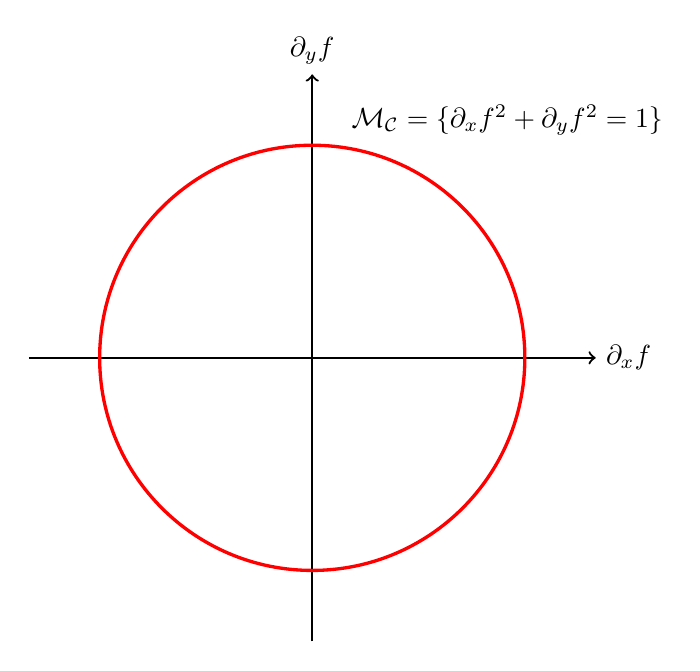
\begin{tikzpicture}[scale=0.9]
%\draw[help lines, color=gray!30, dashed] (-0.9,-0.9) grid (4.9,4.9);
\draw[->, thick] (-4,0)--(4,0) node[right]{$\partial_x f$};
\draw[->, thick] (0,-4)--(0,4) node[above]{$\partial_y f$};
\draw[color=red, very thick](0,0) circle (3);
\node[above] at (2.75,3) {$\mathcal{M}_\mathcal{C}=\{\partial_xf^2+\partial_yf^2=1\}$};
\end{tikzpicture}
\end{subfigure}
\caption{The constraint manifold $\mathcal{M}_\mathcal{C}=\{\partial_xf^2+\partial_yf^2=1\}$ in the space of first order derivatives $(\partial_x f,\partial_yf)$.}\label{fig:constraintManifold}
\end{figure}



%%%%%%%%%%%%%%%%%%%%%%%%%%%%%%%%%%%%%%%%%%%%%%%%%%%%%%%%%%%%%%%%
\section{Constraint initial conditions of the caustic skeleton}\label{sec:caustic_skeleton_constraints}
Given non-linear constrained Gaussian random field theory and the caustic conditions, we study the progenitors of the filaments and clusters in the Zel'dovich approximation. Given the displacement field 
\begin{align}
\bm{s}_t(\bm{q}) = -b_+(t) \nabla_{\bm{q}} \Psi(\bm{q}),
\end{align}
it is convenient to express the deformation tensor
\begin{align}
\bm{\psi}(\bm{q}) = \begin{pmatrix} T_{11}(\bm{q}) & T_{12}(\bm{q}) \\ T_{12}(\bm{q}) & T_{22}(\bm{q})\end{pmatrix}
\end{align}
in terms of the partial derivatives of the displacement potential $T_{ij\dots k}=\frac{\partial}{\partial q_i}\frac{\partial}{\partial q_j}\dots \frac{\partial}{\partial q_k}\Psi$. The eigenvalue and eigenvector fields of $\bm{\psi}$ defined by
\begin{align}
\bm{\psi}(\bm{q}) \bm{v}_i(\bm{q}) = \lambda_i(\bm{q}) \bm{v}_i(\bm{q}),
\end{align}
with the ordering $\lambda_1\geq \lambda_2$. We normalize the eigenvector field to unity, \textit{i.e.}, $\|\bm{v}_{i}\|=1$. We can express the eigenvalue and eigenvector fields explicitly in terms of the second order derivatives of the deformation potential
\begin{align}
\lambda_{1,2} &= \frac{1}{2}\left[T_{11}+T_{22} \pm \sqrt{4 T_{12}^2+(T_{11}-T_{22})^2}\right]\,,\\
\bm{v}_{1,2} &\propto \left(T_{11}-T_{22} \pm \sqrt{4 T_{12}^2+(T_{11}-T_{22})^2}, 2 T_{12}\right)\,,
\end{align}
showing their non-linear dependence on the deformation potential. In the study below, we assume a power-law power spectrum for the gravitational potential
\begin{align}
P(k)=k^{n_s} e^{-\sigma^2 \|\bm{k}\|^2}
\end{align}
with the spectral index $n_s=-1$ and the Gaussian smoothing at the length scale $\sigma = 5 \text{ Mpc}$.

%%%%%%%%%%%%%%%%%%%%%%%%%%%%%%%%%%%%%%%%%%%%%%%%%%%%%%%%%%%%%%%%
\subsection{Cusp filament}
The cusp caustic forming at time $t$, corresponding to the largest eigenvalue field $\lambda_1$, satisfies the conditions
\begin{align}
b_+(t) \lambda_1(\bm{q}_c) &= 1\,, \\
 \bm{v}_1(\bm{q}_c) \cdot \nabla\lambda_1(\bm{q}_c) &= 0\,.
\end{align}
The orientation of the cusp is determined by the normal vector
\begin{align}
\bm{n} =  \nabla(\bm{v}_1(\bm{q}_c) \cdot \nabla\lambda_1(\bm{q}_c))\,,
\end{align}
which makes an angle 
\begin{align}
\alpha = \text{sign}(\bm{v}_2\cdot \bm{n}) \arccos\left(\frac{|\bm{v}_1\cdot \bm{n}|}{\|\bm{n}\|}\right)
\end{align}
with respect the corresponding eigenvector $\bm{v}_1$. As both the cusp curve and the eigenvector field consist of lines, the angle $\alpha$ assumes a value in the interval $[-\pi/2,\pi/2]$. 

In figure \ref{fig:meanCusp}, we plot the mean field of the cusp filament with the condition that centre of the box has a cusp caustic oriented along the vertical direction. The gravitational potential is close to a dipole. The blue central structure yields an inflow of matter, whereas two red structures around the blue structure yield two outflow regions. The critical curve in the eigenvalue field consists of an elongated oval which forms the traditional Zel'dovich pancake in the Zel'dovich approximation. The cusp curve bisects the oval in Lagranian space and the pancake Eulerian space. In the $N$-body simulation, the mass elements virialize around the cups curve.

On average, the orientation of cusp curve is normal to the eigenvector field $\bm{v}_1$. Figure \ref{fig:alpha} plots the distribution  of the angle $\alpha$. The distribution consists of a bell curve centered at $\alpha =0$ and an exponential fall off towards the angles $\alpha =\pm \pi/2$.

\begin{figure}
\centering
\begin{subfigure}[b]{0.32\textwidth}
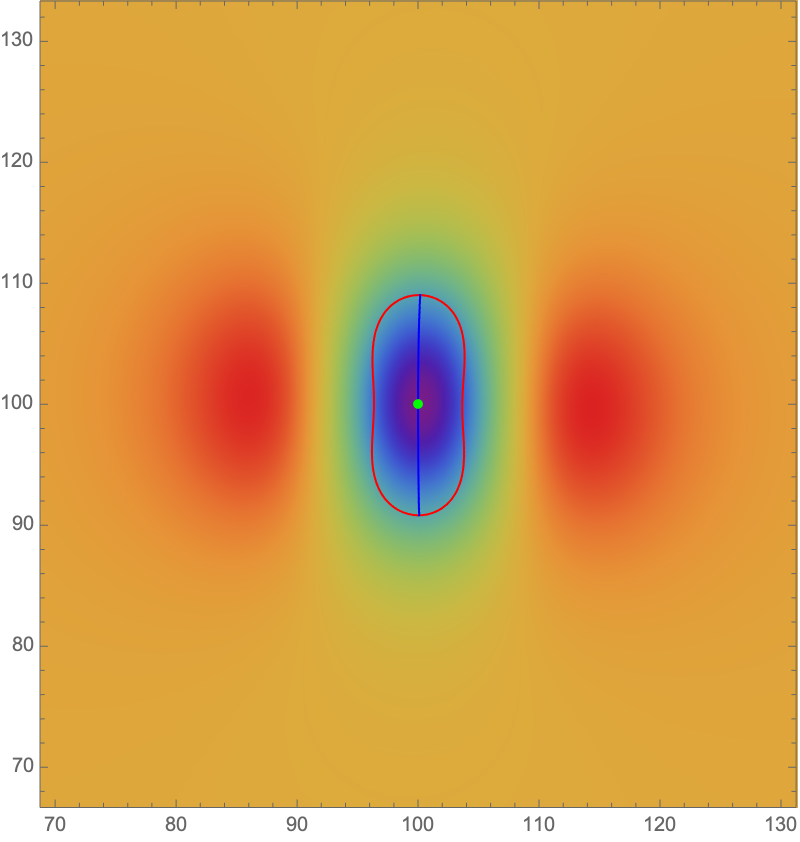
\includegraphics[width=\textwidth]{Cusp_mean_Phi}
\end{subfigure}~
\begin{subfigure}[b]{0.32\textwidth}
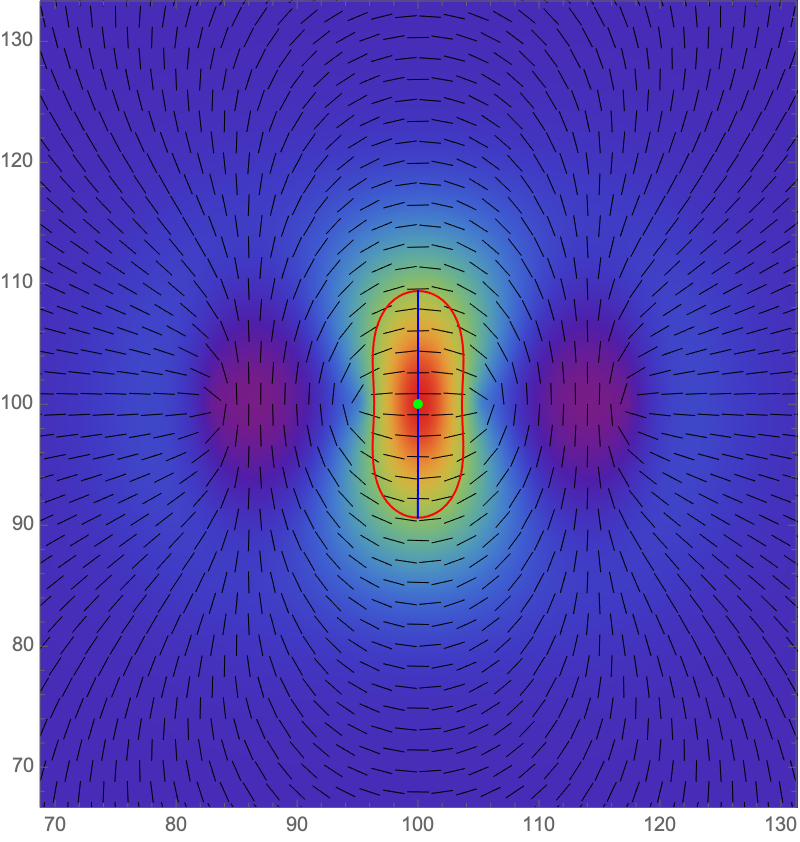
\includegraphics[width=\textwidth]{Cusp_mean_L}
\end{subfigure}~
\begin{subfigure}[b]{0.32\textwidth}
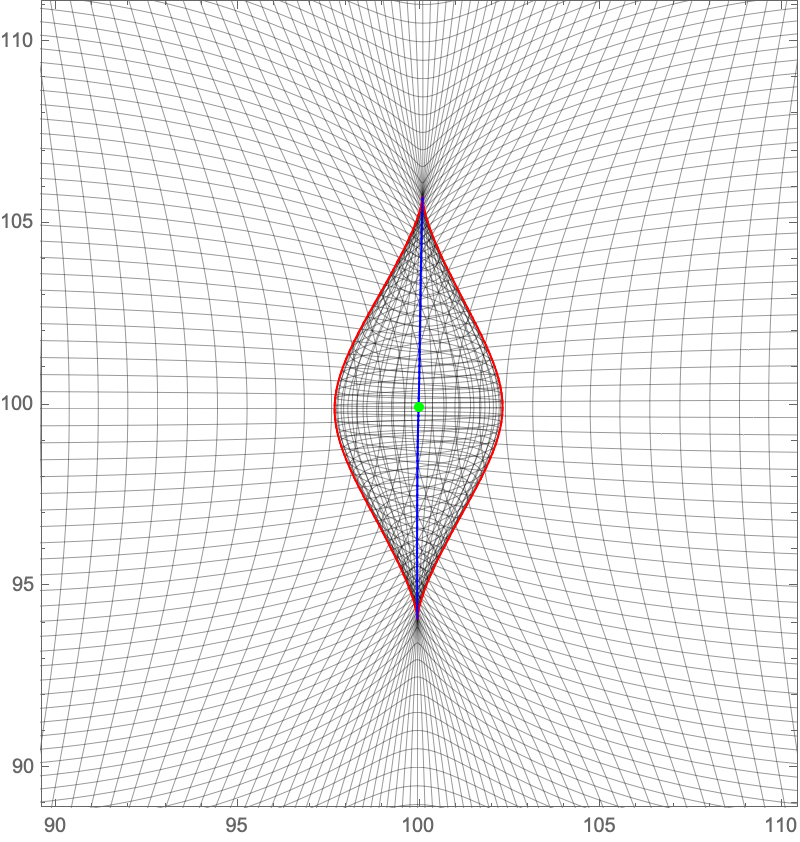
\includegraphics[width=\textwidth]{Cusp_mean_Z}
\end{subfigure}
\caption{The mean cusp caustic. \text{Left:} the gravitational potential. \textit{Centre:} the first eigenvalue and eigenvector fields. \textit{Right:} The Zel'dovich approximation}\label{fig:meanCusp}
\end{figure}

\begin{figure}
\centering
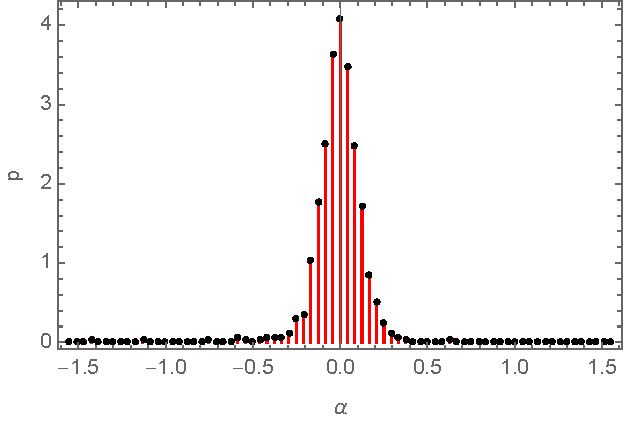
\includegraphics[width=0.5\textwidth]{alpha}
\caption{The distribution of the angle $\alpha$} 
\label{fig:alpha}
\end{figure}

%%%%%%%%%%%%%%%%%%%%%%%%%%%%%%%%%%%%%%%%%%%%%%%%%%%%%%%%%%%%%%%%
\subsubsection{Sampling the constraint manifold}
To analyze the constraint field of the cusp caustic, we work in the eigenframe of the deformation tensor for which $\bm{v}_1=(1,0)$ and $\bm{v}_2=(0,1)$. In this frame, the caustic conditions yield a set of linear conditions on the second and third order derivatives of the deformation potential
\begin{align}
T_{11}=1/b_+(t)\,, \quad T_{12}=0\,,\quad T_{22}\leq T_{11}\,,\quad T_{111}=0\,.\label{eq:cusp_cond_1}
\end{align}
The normal vector yields the non-linear form
\begin{align}
\bm{n}=\left(T_{1111} + \frac{3T_{112}^2}{T_{11}-T_{22}}, T_{1112} + \frac{3T_{112}T_{122}}{T_{11}-T_{22}}\right)\,.\label{eq:cusp_cond_2}
\end{align}
For a derivation of these identities see appendix \ref{ap:eigenvalueRel}.

For simplicity, let's first ignore the orientation of the cusp curve and consider a cusp curve passing through the center of the box, with the relevant linear statistics $Y=(T_{11},T_{12},T_{22},T_{111})$, whose probability density factorizes into the density of the joint distribution of $T_{11}$ and $T_{22}$ and the one-dimensional Gaussian distributions for $T_{12}$ and $T_{111}$, \textit{i.e.},
\begin{align}
p(T_{11},T_{12},T_{22},T_{111}) = p(T_{11},T_{22})p(T_{12})p(T_{111})\,.
\end{align}
Generally, two derivatives of a Gaussian random field at a point are independent if and only if they together consist of an odd number of derivatives in either the $q_1$ or the $q_2$ direction. The conditional probability density takes the form
\begin{align}
p&(T_{11},T_{12},T_{22},T_{111}|,T_{22}\leq T_{11}=1/b_+,T_{12}=0,T_{111}=0) \\
&= p(T_{22}| T_{22} \leq T_{11}=1/b_+)\\
&= \mathcal{N} e^{-\frac{3(T_{11} + T_{22})^2 - 8 T_{11} T_{22}}{2 \sigma_2^2}}\big|_{T_{11}=1/b_+}\,,
\end{align}
with the normalization constant $\mathcal{N}$. After sampling $T_{22}$ from this distribution, we can use linear constrained random field theory to obtain the corresponding realization. Note that this procedure is equivalent to generating realizations for the linear constraints $T_{11}=1/b_+,T_{12}=T_{111}=0$ and rejecting realizations for which $T_{22} > 1/b_+$. Give these realizations, it is straightforward to compute the angle $\alpha$ and sample the distribution (see figure \ref{fig:alpha}).

The orientation of the cusp curve is fully characterized by the derivatives  
\begin{align}
Y=(T_{11},T_{12},T_{22},T_{111},T_{112},T_{122},T_{1111},T_{1112})
\end{align}
with the conditional distribution
\begin{align}
&p(T_{11},T_{12},T_{22},T_{111},T_{112},T_{122},T_{1111},T_{1112}|T_{22} \leq T_{11}=1/b_+, T_{111}=0)\\
&=
p(T_{11},T_{22},T_{1111}|T_{22}\leq T_{11}=1/b_+)p(T_{12}T_{1112}|T_{12}=0)p(T_{111},T_{122}|T_{111}=0)p(T_{112})\,.
\end{align}
We can generate realizations for which the cusp curve is vertical in the centre of the box, by sampling this distribution with the additional constraint that $\bm{n} \propto (1,0)$. However, for this paper, we will use the a slightly different method based on the sampling method described above. Given an realization, we first evaluate all second, third, and fourth order derivatives and evaluate the angle $\alpha$. Subsequently, rotate these derivatives by an angle $\alpha$ (following appendix \ref{ap:rotations}). The resulting derivatives form a representative sample of a cusp curve running vertical through the centre of the box. By generating a linear constraint realizations with these rotates derivatives, we obtain a realization of the Gaussian random field required cusp curve.

%
%\begin{figure}
%\centering
%\begin{subfigure}[b]{0.32\textwidth}
%\includegraphics[width=\textwidth]{Cusp_mean}
%\caption{$\text{mean}(\Psi)$}
%\end{subfigure}~
%\begin{subfigure}[b]{0.32\textwidth}
%\includegraphics[width=\textwidth]{Cusp_variance}
%\caption{$\text{variance}(\Psi)$}
%\end{subfigure}~
%\begin{subfigure}[b]{0.32\textwidth}
%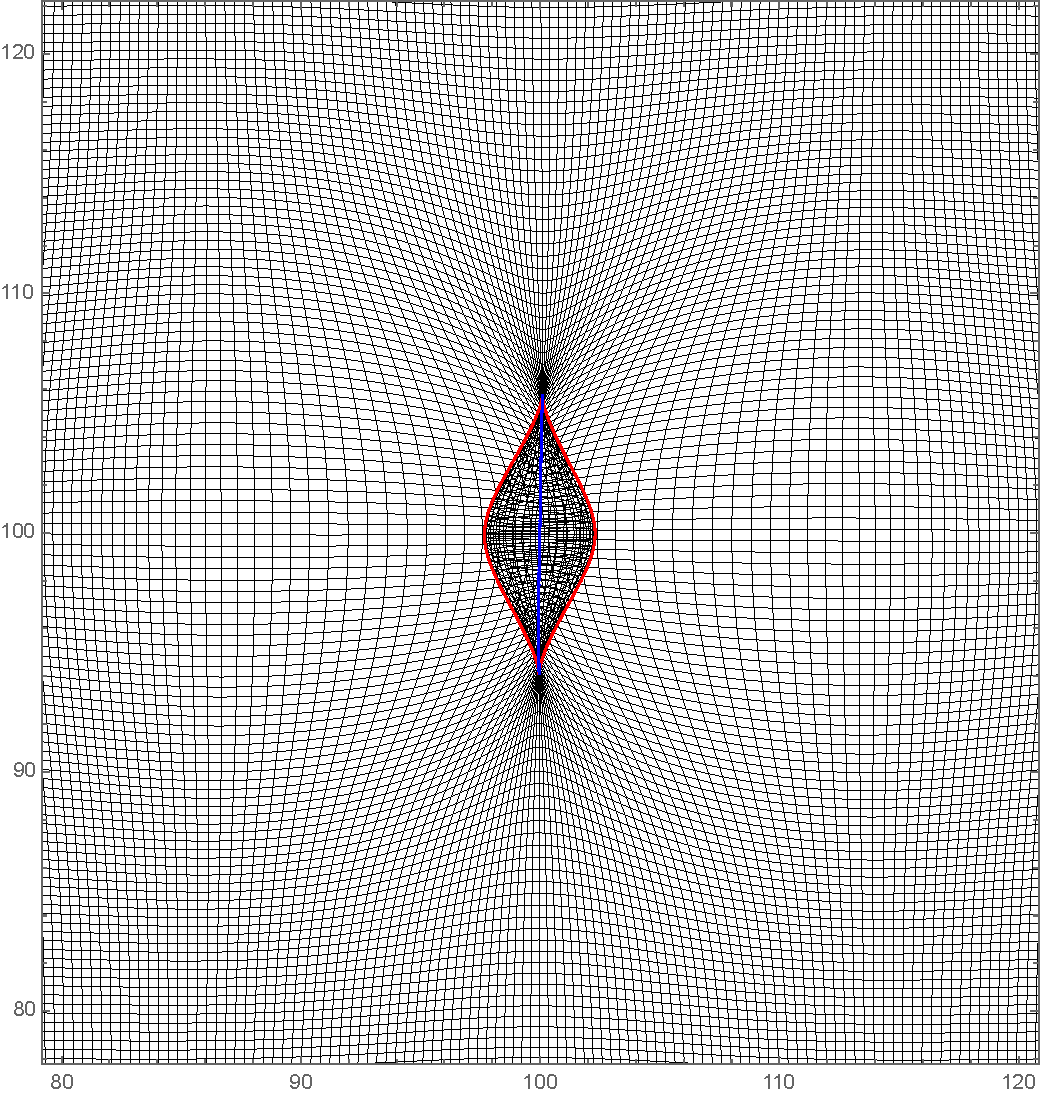
\includegraphics[width=\textwidth]{Cusp_E_Mean}
%\caption{Zel'dovich}
%\end{subfigure}
%\caption{The mean and variance field of the cusp filament}\label{fig:meanCusp}
%\end{figure}





%%%%%%%%%%%%%%%%%%%%%%%%%%%%%%%%%%%%%%%%%%%%%%%%%%%%%%%%%%%%%%%%
\subsection{Swallowtail cluster}
The swallowtail caustic forming at time $t$, corresponding to the largest eigenvalue field $\lambda_1$, satisfies the conditions
\begin{align}
b_+(t) \lambda_1(\bm{q}_c) = 1\,,\\
\quad \bm{v}_1(\bm{q}_c) \cdot \nabla\lambda_1(\bm{q}_c) = 0\,,\\
 \quad\bm{v}_1(\bm{q}_c)\cdot \nabla( \bm{v}_1(\bm{q}_c) \cdot \nabla\lambda_1(\bm{q}_c)) = 0\,.
\end{align}
The cusp curve in the swallowtail caustic is parallel to the eigenvector field $\bm{v}_1$ since $\bm{v}_1 \cdot \bm{n}=0$ or equivalently $\alpha = \pm \pi/2$. The swallowtail caustic does not require us to fix its orientation. However, we do need to specify the direction, normal to the fold curve, in which the swallowtail structure forms. We will here use the condition $\bm{v}_2 \cdot \nabla \lambda_1(\bm{q}) <0$.





In figure \ref{fig:meanSwallowtail}, we plot the mean field of the swallowtail cluster. The gravitational potential is again close to a dipole. However, note the development of an asymmetry with respect to the horizontal axis. The blue central structure yields an inflow of matter, whereas two red structures around the blue structure yield two outflow regions. The critical curve in the eigenvalue field consists of an elongated oval with two bifurcation in the upper half plane. The cusp curves form a trident inside the fold curve. In the Zel'dovich approximation, the caustic skeleton consists of a Zel'dovich pancake with two whiskers in the upper half plane. In the $N$-body simulation, the mass elements virialize around the cusp curves.



\begin{figure}
\centering
\begin{subfigure}[b]{0.32\textwidth}
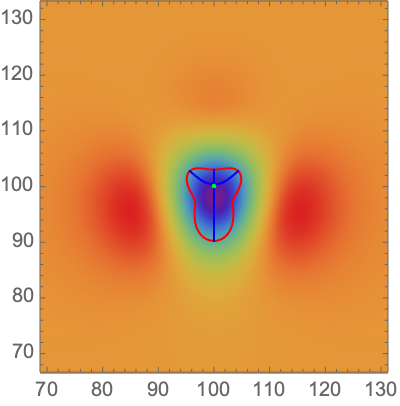
\includegraphics[width=\textwidth]{Swallowtail_mean_Phi}
\end{subfigure}~
\begin{subfigure}[b]{0.32\textwidth}
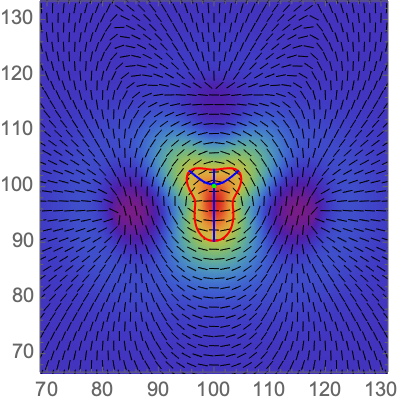
\includegraphics[width=\textwidth]{Swallowtail_mean_L}
\end{subfigure}~
\begin{subfigure}[b]{0.32\textwidth}
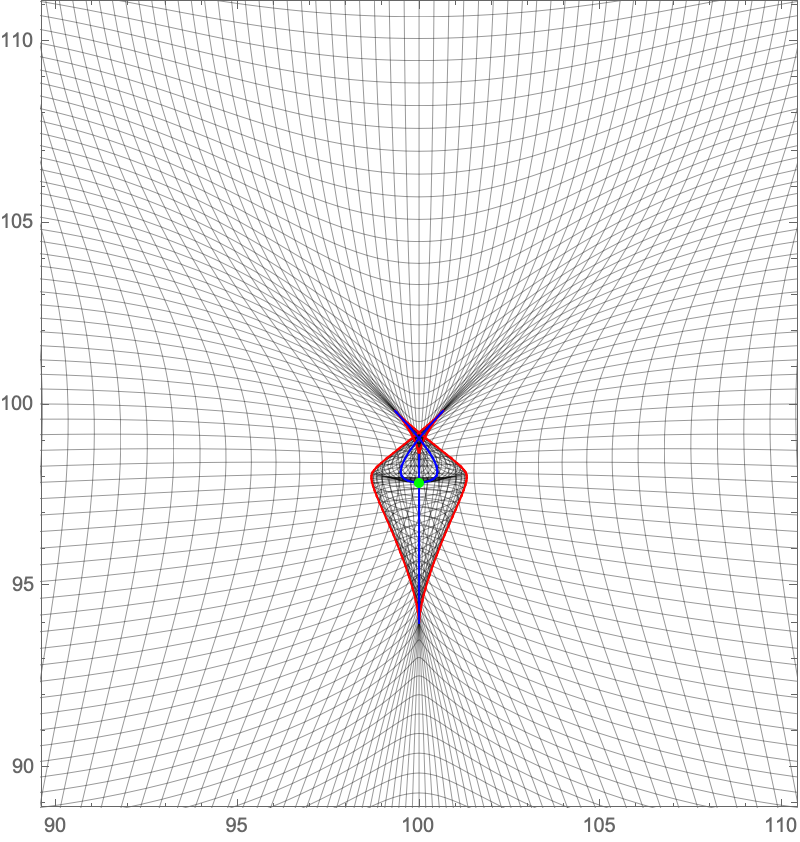
\includegraphics[width=\textwidth]{Swallowtail_mean_Z}
\end{subfigure}
\caption{The mean swallowtail caustic. \text{Left:} the gravitational potential. \textit{Centre:} the first eigenvalue and eigenvector fields. \textit{Right:} The Zel'dovich approximation}\label{fig:meanSwallowtail}
\end{figure}


%%%%%%%%%%%%%%%%%%%%%%%%%%%%%%%%%%%%%%%%%%%%%%%%%%%%%%%%%%%%%%%%
\subsubsection{Sampling the constraint manifold}
In the eigenframe, the caustic conditions for the cusp take the form
\begin{align}
T_{11}=1/b_+(t)\,, \quad T_{12}=0\,,\quad T_{22}\leq T_{11}\,,\quad T_{111}=0\,, \quad T_{1111}+\frac{3T_{112}^2}{T_{11}-T_{22}} =0\,.
\end{align}
The condition that specifies the direction in which the swallowtail develops, $\bm{v}_2 \cdot \nabla \lambda_1  <0$, yields the simple form 
\begin{align}
T_{112} <0\,.
\end{align}
See appendix \ref{ap:eigenvalueRel} for a detailed derivation. 

The swallowtail caustic is determined by the linear statistics $Y=(T_{11},T_{12},T_{22},T_{111},T_{112},T_{1111})$ with the probability density
\begin{align}
p(T_{11},T_{12},T_{22},T_{111},T_{112},T_{1111})=p(T_{11},T_{22},T_{1111})p(T_{12})p(T_{111})p(T_{112})\,,
\end{align}
and the constraint distribution 
\begin{align}
&p\left(T_{22},T_{112},T_{1111}|T_{22}\leq T_{11}=1/b_+, T_{12}=0,T_{111}=0,T_{1111}+\frac{3T_{112}^2}{T_{11}-T_{22}}=0\right)\\
=&\, p\left(T_{22},T_{112}, T_{1111}|T_{22}\leq T_{11}=1/b_+, T_{1111}+\frac{3T_{112}^2}{T_{11}-T_{22}}=0\right)\,.
\end{align}

For the cusp caustic, it sufficed to construct realizations with the linear constraints $T_{11}=1/b_+$, $T_{12}=0$, $T_{111}=0$ and reject realizations for which $T_{22} > T_{11}$. For the swallowtail caustic, we implement a more advanced rejection scheme to efficiently sample the constrained manifold.

In the joint distribution of the statistic $(T_{11},T_{22},T_{112},T_{1111})$, the variable $T_{112}$ is independent of the statistics $T_{11}, T_{22}$ and $T_{1111}$. Moreover, note that the conditions $T_{1111}+\frac{3T_{112}^2}{T_{11}-T_{22}}=0$ and $T_{112}<0$ fully specify $T_{112}$ in terms of the variables $T_{11},T_{22}$ and $T_{1111}$. We use these properties to construct a rejection sampling scheme in which we sample the Gaussian distribution for $(T_{22},T_{1111})$ and accept a sample with a probability determined by the joint distribution for $(T_{22},T_{112},T_{1111})$.

Consider the Gaussian joint distribution $p(T_{11},T_{22},T_{1111})$ with vanishing mean $\bm{\mu}=\bm{0}$ and the covariance matrix $\begin{pmatrix} a & \bm{b} \\ \bm{b}^T & \Sigma \end{pmatrix}$ consisting of the elements
\begin{align}
a=\frac{3 \sigma_2^2}{8}\,, \quad
\bm{b}=\left(\frac{\sigma_2^2}{8}, -\frac{5 \sigma_3^2}{16}\right)\,,\quad
\Sigma = \begin{pmatrix} \frac{3 \sigma_2^2}{8} & -\frac{\sigma_3^2}{16} \\ -\frac{\sigma_3^2}{16} & \frac{35 \sigma_4^2}{128}\end{pmatrix}, 
\end{align}
and the independent statistics $T_{112}$, which is normally distributed with zero mean $\langle T_{112}\rangle = 0$ and variance $\langle T_{112}^2\rangle = \sigma_3^2/16$. The conditional distribution $p(T_{22},T_{1111}|T_{11}=1/b_+)$ is a bivariate Gaussian distribution with non-zero mean $\bar{\bm{\mu}}=\frac{\bm{b}}{a b_+}$ and the covariance matrix $\bar{\Sigma}=\Sigma -\frac{1}{a} \bm{b}\bm{b}^T$. After sampling from this distribution, we first reject samples for which $T_{22}>1/b_+$ or $T_{1111}>0$ to obtain samples from the auxiliary probability density 
\begin{align}
p(T_{22},T_{1111}| T_{22} < T_{11}=1/b_+,T_{1111}\leq 0)\,.
\end{align}

 The variables $T_{22},T_{1111}$ fully determine the variable $T_{112}$,
\begin{align}
T_{112}= -\sqrt{-\frac{T_{1111}(T_{11}-T_{22})}{3}}\,,
\end{align}
when $T_{22} < T_{11}$ and $T_{1111}\leq 0$.  The unnormalized conditional density is the product of the conditional density $p(T_{22},T_{1111}|T_{22}\leq T_{11}=1/b_+,T_{1111}\leq 0)$ and a function assuming values between $0$ and $1$,
\begin{align}
&p(T_{22},T_{1111}|T_{22}\leq T_{11}=1/b_+, T_{1111}+3T_{112}^2/(T_{11}-T_{22}) =0)\\
& \propto e^{-\frac{1}{2}((T_{22},T_{1111})-\bar{\bm{\mu}})\bar{\Sigma}^{-1}((T_{22},T_{1111})-\bar{\bm{\mu}}) }\Theta(1/b_+-T_{22})\Theta(-T_{1111})e^{ \frac{8T_{1111} (1/b_+ - T_{22})}{3 \sigma_3^2}}
\end{align}
with the Heaviside step function $\Theta$. Hence, we obtain samples of the target distribution by sampling from the conditional density $p(T_{22},T_{1111}|T_{22}\leq T_{11}=1/b_+,T_{1111}\leq 0)$ and accepting samples with probability 
\begin{align}
\exp\left[ \frac{8T_{1111} (1/b_+ - T_{22})}{3 \sigma_3^2}\right]\,.
\end{align}


%%%%%%%%%%%%%%%%%%%%%%%%%%%%%%%%%%%%%%%%%%%%%%%%%%%%%%%%%%%%%%%%
\subsection{Umbilic cluster}
The umbilic caustic forming at time $t$ satisfies the conditions
\begin{align}
b_+(t) \lambda_1(\bm{q}_c) = b_+(t) \lambda_2(\bm{q}_c) = 1\,.
\end{align}
In terms of the second order derivatives of the displacement potential, these eigenvalue conditions can be expressed in terms of three linear conditions
\begin{align}
T_{11}&=T_{22}=1/b_+(t)\,,\\
T_{12}&=0\,.
\end{align}
At the umbilic points, the determinant 
\begin{align}
\det(\nabla \bm{x}_t) = \det (I- b_+ \bm{\psi})
\end{align}
assumes a critical point, whose nature is determined by the Hessian
\begin{align}
\mathcal{H}\left[\det (I- b_+ \bm{\psi})\right] =
\begin{pmatrix} 
2(T_{111}T_{122} -T_{112}^2) & T_{111}T_{222}-T_{112}T_{122} \\
T_{111}T_{222}-T_{112}T_{122} & 2(T_{112}T_{222}-T_{122}^2)
\end{pmatrix}\,,
\end{align}
and its determinant
\begin{align}
&\det\left( \mathcal{H}\left[\det (I- b_+ \bm{\psi})\right]\right) \\
&=
 6 T_{111} T_{112} T_{122} T_{222} + 3 T_{112}^2 T_{122}^2  - 4 (T_{111} T_{122}^3 + T_{112}^3 T_{222})  - T_{111}^2 T_{222}^2\,,
\end{align}
see \cite{Rozhanskii:1984}. Note that the Hessian at the critical point only depends on the third order derivatives of the deformation potential. The fourth order derivatives cancel when $T_{11}=T_{22}=1/b_+$ and $T_{12}=0$. The umbilic point is an elliptic caustic $D_4^+$ when the critical point is a maximum, or a minimum, \textit{i.e.}, for which 
\begin{align}
\det (\mathcal{H}\left[\det (I- b_+ \bm{\psi})\right]) >0\,.
\end{align}
The umbilic point is an hyperbolic caustic when the critical point is a saddle point, \textit{i.e.},
\begin{align}
\det (\mathcal{H}\left[\det (I- b_+ \bm{\psi})\right]) <0\,.
\end{align}
This condition should be contrasted with the condition presented in \cite{Delmarcelle:1995, Lavin:1997, Hidding:2016, Feldbrugge:2018} based on the sign of 
\begin{align}
\delta = \frac{1}{2}(T_{111} T_{122} + T_{112} T_{222} - T_{112}^2  - T_{122}^2 ).
\end{align} 
In fact, this condition describes the behaviour of the eigenvector field in the vicinity of the umbilic point and does not differentiates between the elliptic and hyperbolic caustics. Note that for the elliptic caustic we always have $\delta <0$.


\begin{figure}
\centering
\begin{subfigure}[b]{0.32\textwidth}
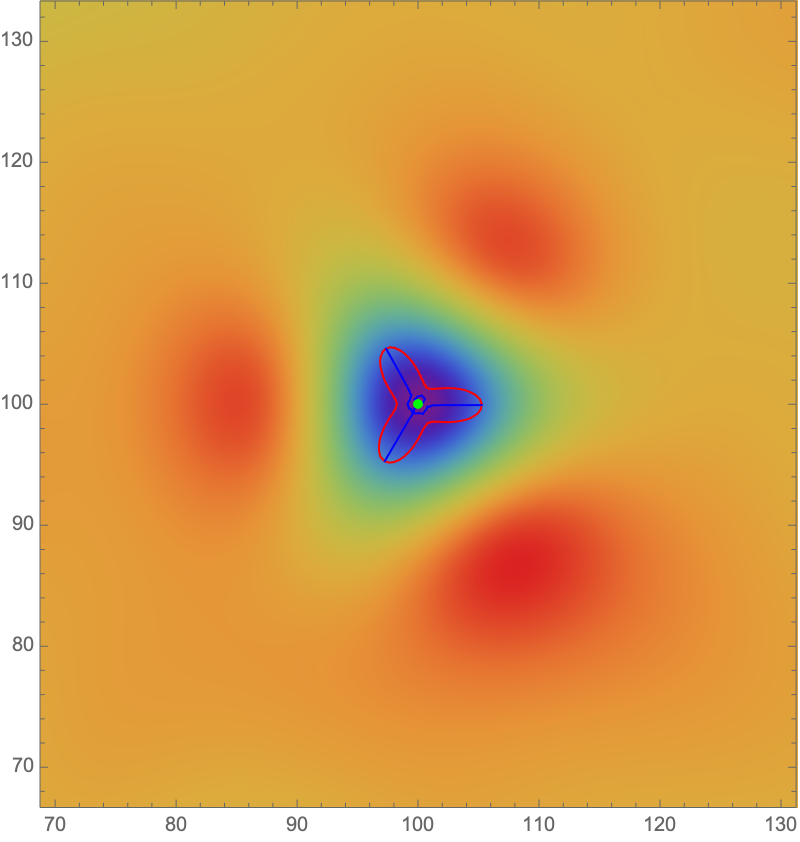
\includegraphics[width=\textwidth]{Elliptic_mean_Phi}
\end{subfigure}~
\begin{subfigure}[b]{0.32\textwidth}
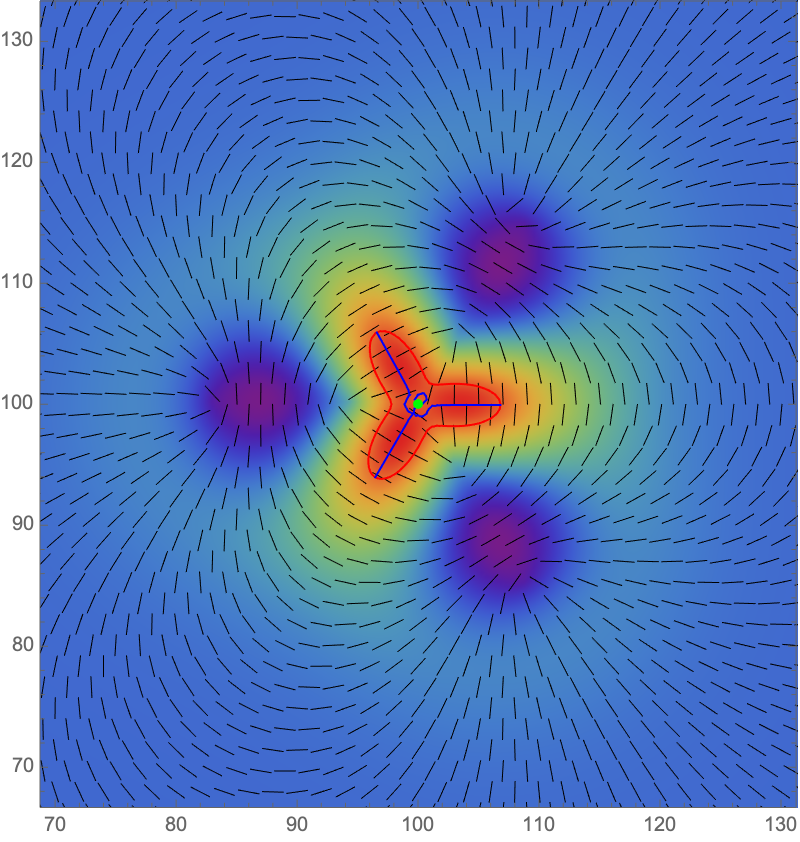
\includegraphics[width=\textwidth]{Elliptic_mean_L}
\end{subfigure}~
\begin{subfigure}[b]{0.32\textwidth}
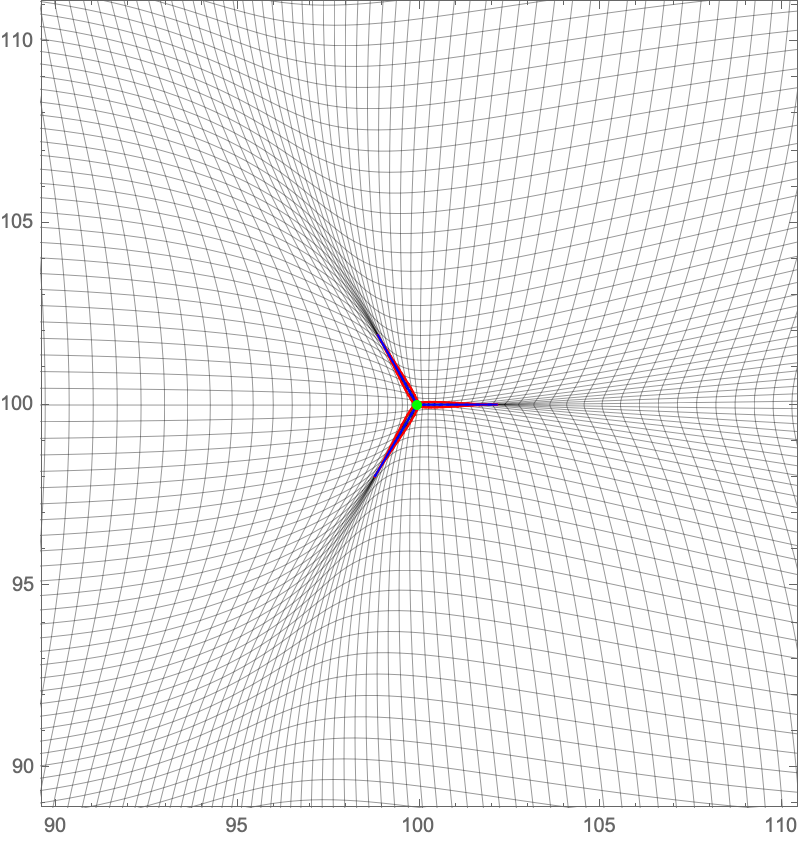
\includegraphics[width=\textwidth]{Elliptic_mean_Z}
\end{subfigure}\\
\begin{subfigure}[b]{0.32\textwidth}
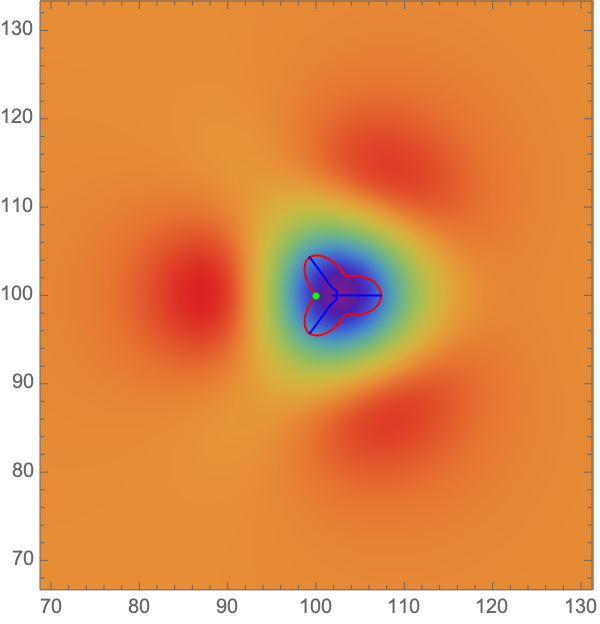
\includegraphics[width=\textwidth]{Hyperbolic_mean_Phi}
\end{subfigure}~
\begin{subfigure}[b]{0.32\textwidth}
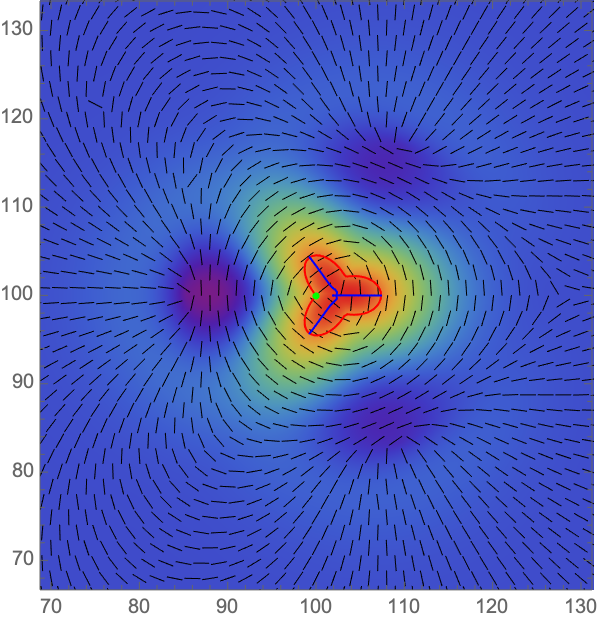
\includegraphics[width=\textwidth]{Hyperbolic_mean_L}
\end{subfigure}~
\begin{subfigure}[b]{0.32\textwidth}
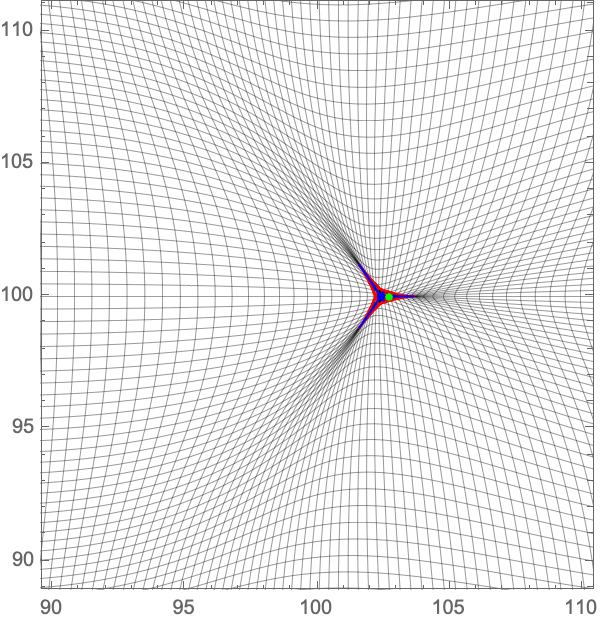
\includegraphics[width=\textwidth]{Hyperbolic_mean_Z}
\end{subfigure}
\caption{The mean umbilic caustic. \textit{Upper:} the  elliptic caustic. \textit{Lower:} the hyperbolic caustic. \textit{Left:} the gravitational potential. \textit{Centre:} the first eigenvalue and eigenvector fields. \textit{Right:} The Zel'dovich approximation}\label{fig:meanHyperbolic}
\end{figure}

More generally, expand the displacement field $\bm{s}_t$ to quadratic order in $q_1$ and $q_2$ around a umbilic point at the origin $(q_1,q_2)=(0,0)$. The determinant of the gradient $\nabla \bm{x}_t$ has a critical point at the origin, as it is the product of two eigenvalue fields that vanish at the origin. The determinant takes the general form
\begin{align}
\det \nabla \bm{x}_t&=\det(I + \nabla \bm{s}_t)\\
&= 
A q_1^2 + B q_1 q_2 + C q_2^2 + O(q_1^3,q_1^2 q_2,q_1 q_2^2,q_2^3)\,.
\end{align}
for some constants $A,B,$ and $C$.
%with
%\begin{align}
%A&= s_{1,11} s_{2,12}-s_{1,12} s_{2,11}\,,\\
%B&= s_{1,11} s_{2,22}-s_{1,22} s_{2,11}\,,\\
%C&= s_{1,12} s_{2,22}-s_{1,22} s_{2,12}\,, 
%\end{align}
%where we write the displacement field as $\bm{s}_t=(s_1,s_2)$ and the partial derivatives as $s_{i,jk}=\partial_j \partial_k s_{i}$. 
For small $q_1$ and $q_2$, the level set $\det \nabla \bm{x}_t =0$ approaches a conic section:
\begin{itemize}
\item an ellipse when the discriminant $B^2 - 4AC$ is negative corresponding to the $D_4^+$ caustic,
\item a hyperbole when the discriminant $B^2 - 4AC$ is positive corresponding to the $D_4^-$ caustic,
\item a parabola when the discriminant $B^2 - 4AC$ vanishes, corresponding to the $D_5$ caustic (which does not feature in the 2D cosmic web).
\end{itemize}
Note that the discriminant coincides with the negative of the determinant of the Hessian, \textit{i.e.},
\begin{align}
B^2-4AC = -\det \left(\mathcal{H} \left[\det \nabla \bm{x}_t \right]\right)\,.
\end{align}
When the displacement field is a gradient field, the constants $D$ and $E$ vanish and the condition reduces to the constant discussed above.


The orientation of the elliptic umbilic caustic is determined by the behaviour of the eigenvector fields of the deformation tensor in the vicinity of the caustic. The fold curve in the vicinity of the elliptic umbilic caustic is a small ellipse, which forms three cusp caustics when the eigenvector field is parallel to the eigenvector field, $\bm{v}_i \cdot \bm{m} = 0$ with $\bm{m}$ the vector normal to this circle.

The orientation and configuration of the hyperbolic umbilic caustic is determined by the eigenvalues $\nu_i$ and eigenvectors $\bm{w}_i$ of the Hessian $\mathcal{H}\left[\det (I- b_+ \bm{\psi})\right]$. The cusp curve of the hyperbolic umbilic is directed towards the eigenvector corresponding to the positive eigenvalue. The angle $\beta = 2 \arctan(\sqrt{|\nu_1/\nu_2|})$ describes the angle between the two wedges of the fold curves. 


In figure \ref{fig:meanHyperbolic}, we plot the mean field of the elliptic and the swallowtail caustic. Observe that the umbilic caustics join three cusp curves and are naturally associated to the clusters of the cosmic web.




%%%%%%%%%%%%%%%%%%%%%%%%%%%%%%%%%%%%%%%%%%%%%%%%%%%%%%%%%%%%%%%%
\subsubsection{Sampling the constraint manifold}
We implement the umbilic caustics by sampling random fields with the linear constraints
\begin{align}
T_{11}&=T_{22}=1/b_+\,,\\
T_{12}&=0\,.
\end{align}
We subsequently determine the sign of the determinant $\det\left( \mathcal{H}\left[\det (I- b_+ \bm{\psi})\right]\right)$ to identify whether it is an elliptic or an hyperbolic caustic. Given the identification, we compute its orientation. By rotating the second order and third order derivatives (using appendix \ref{ap:rotations}), we generate linear constraint conditions corresponding to elliptic and hyperbolic caustics with a specified orientation. Given the appropriate sampling of the constraint manifold $\mathcal{M}_\mathcal{C}$, we can evaluate the mean field, the variance of the residue and representative realiations.



%%%%%%%%%%%%%%%%%%%%%%%%%%%%%%%%%%%%%%%%%%%%%%%%%%%%%%%%%%%%%%%%
\section{Composite constraint realizations}
To study the interplay between the voids, walls, filaments and clusters in the cosmic web and study the connectivity, it is important to extend constraint theory of the caustic skeleton to include multiple constraints with specified orientations. In this section, we show how to construct realizations with composite constraints.

%%%%%%%%%%%%%%%%%%%%%%%%%%%%%%%%%%%%%%%%%%%%%%%%%%%%%%%%%%%%%%%%
\subsection{Orienting constraint conditions}\label{sec:orientation}
In section \ref{sec:caustic_skeleton_constraints}, we demonstrated a method to construct realizations of Gaussian random fields satisfying a caustic constraint at a single point with a fixed orientation. For example, we constructed realizations which included a cusp filament running vertically through the origin of the initial conditions. From the formalism, it follows that the caustic constraint can be translated to any point in the box by shifting the underlying linear functionals $\bm{C}$ (the Fourier transform of the constraints receives a phase shift). Alternatively, we can generate a realization with a cusp at the origin and translate the origin to the required location using the symmetry of the torus on which the realization lives. Unfortunately, the later method does not work when considering multiple caustic constraints at different locations. Moreover, the second method yields difficulties for even a single caustic constraint when attempting to change the orientation with a rotation due to the symmetries of the boundary conditions of the box.

Fortunately, there exists a efficient method to generate realizations with any preferred orientation at any location:
\begin{enumerate}
\item 
Generate a realization satisfying the caustic conditions at a given point in the box with a fixed orientation as described in section \ref{sec:caustic_skeleton_constraints}. 
\item 
Analyse the orders of the derivatives in the caustic conditions. For example, from equations \eqref{eq:cusp_cond_1} and \eqref{eq:cusp_cond_2}, we note that the cusp caustic is fully determined by a number of second, third, and fourth order derivatives.
\item
Evaluate all derivatives of the realization to the relevant order. Generally, some derivatives were obtained while sampling the constraint manifold $\mathcal{M}_\mathcal{C}$. Others do not directly influence the caustic, and are sampled from the realization. For the cusp, we evaluate the partial derivatives 
\begin{align}
T_{11},T_{12},T_{22},T_{111},T_{112},T_{122},T_{222},T_{1111},T_{1112},T_{1122},T_{1222},T_{2222}\,.
\end{align}
Alternatively, we can extend the constraint manifold to include all these partial derivatives and sample them directly.
\item 
While rotating the coordinate system by an angle $\theta$, the $n$-th order derivatives transform into each other (see appendix \ref{ap:rotations}). We use these transformation rules to obtain a representative sample of the required partial derivatives for the caustic with the desired orentation.
\item 
Finally, we apply the Hoffman Ribak algorithm, with respect to the linear constraints consisting of the relevant partial derivatives, to obtain a realization satisfying the caustic condition with the desired orientation.
\end{enumerate}

See figure \ref{fig:rotation} for an illustration of the cusp caustic with three orientations. In the left panel, the cusp caustic passes vertically through the centre of the box. In the central and right panels, we generate realizations for which the cusp curve passes diagonally and horizontally through the the center of the box. These three realizations share a single unconstrained random field. As a consequence, we see that the structure of the initial conditions away from the centre $(100,100)$ remains unchanged. Using constrained Gaussian random field theory, we can locally tweak the random field to satisfy the desired non-linear constraints.

\begin{figure}
\centering
\begin{subfigure}[b]{0.32\textwidth}
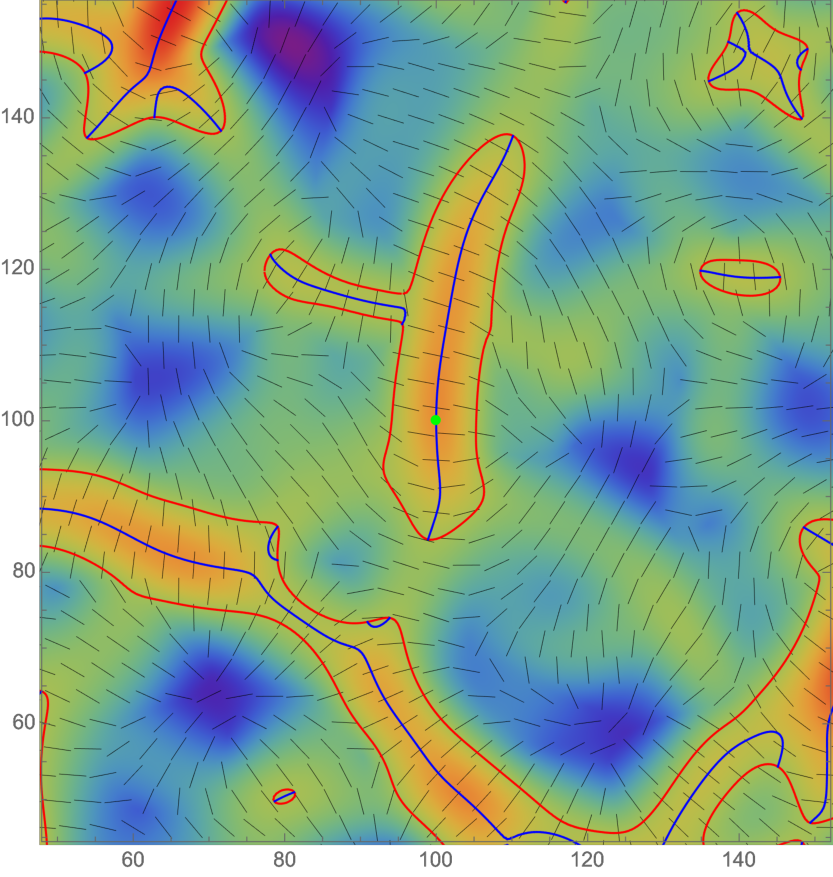
\includegraphics[width=\textwidth]{Rotation_L_1}
\end{subfigure}~
\begin{subfigure}[b]{0.32\textwidth}
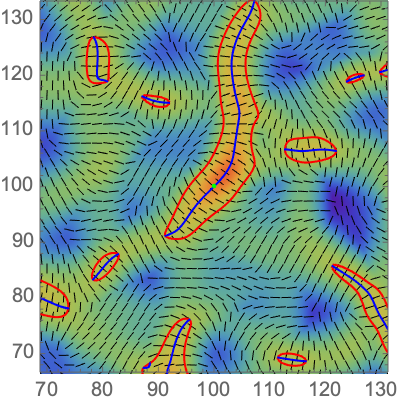
\includegraphics[width=\textwidth]{Rotation_L_2}
\end{subfigure}~
\begin{subfigure}[b]{0.32\textwidth}
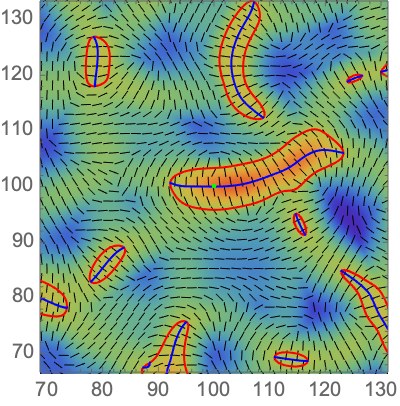
\includegraphics[width=\textwidth]{Rotation_L_3}
\end{subfigure}\\
\begin{subfigure}[b]{0.32\textwidth}
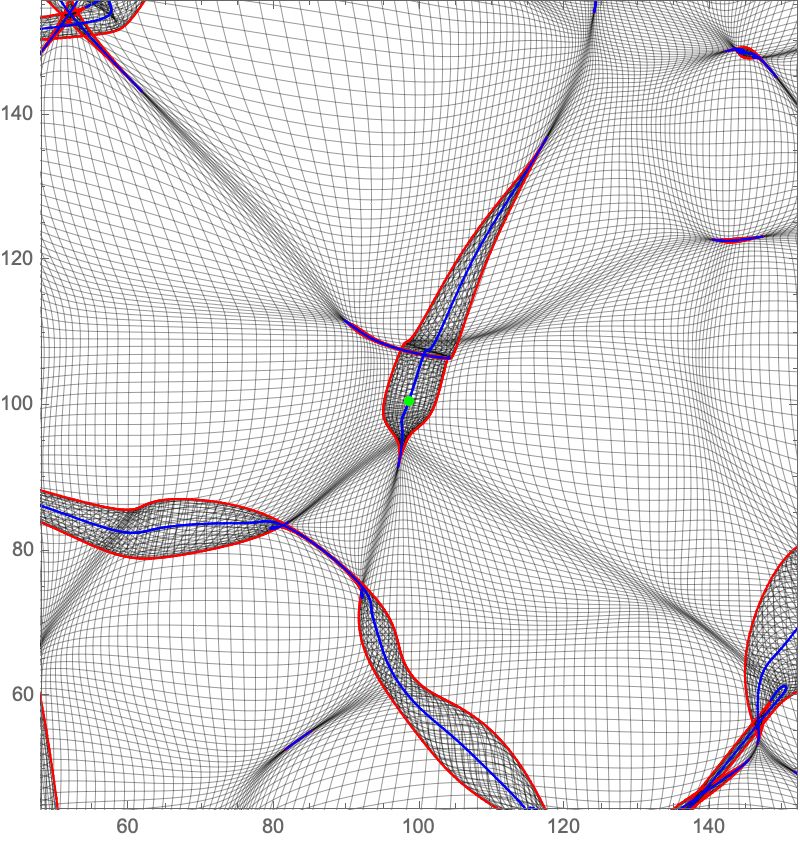
\includegraphics[width=\textwidth]{Rotation_Z_1}
\end{subfigure}~
\begin{subfigure}[b]{0.32\textwidth}
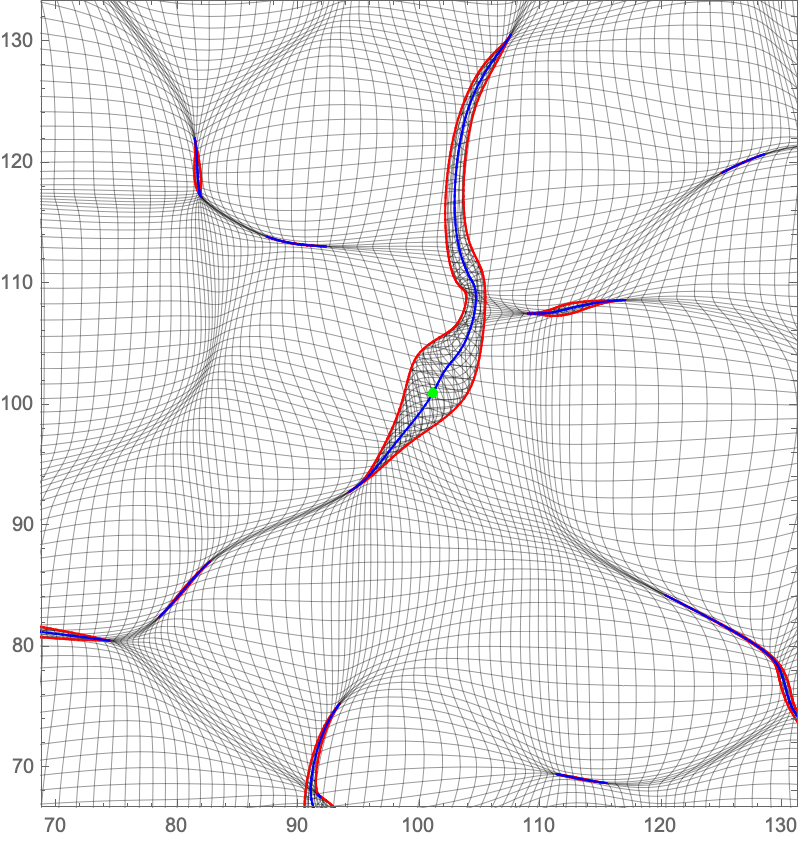
\includegraphics[width=\textwidth]{Rotation_Z_2}
\end{subfigure}~
\begin{subfigure}[b]{0.32\textwidth}
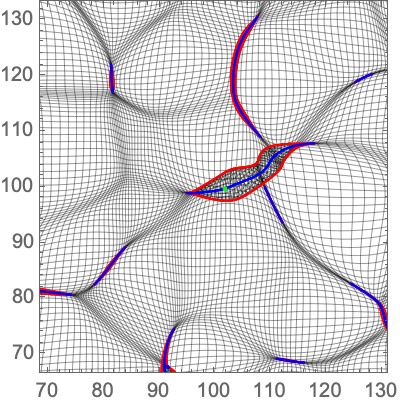
\includegraphics[width=\textwidth]{Rotation_Z_3}
\end{subfigure}
\caption{Rotation of the cusp caustic. \textit{Upper:} the eigenvalue and eigenvector fields in Lagrangian space. \textit{Lower:} the Zel'dovich approximation in Eulerian space. \textit{Left:} with the vertical orientation. \textit{Center:} with a diagonal orientation. \textit{Right:} with the horizontal orientation.}\label{fig:rotation}
\end{figure}


%%%%%%%%%%%%%%%%%%%%%%%%%%%%%%%%%%%%%%%%%%%%%%%%%%%%%%%%%%%%%%%%
\subsection{Multiple constraints}
In section \ref{sec:orientation}, we showed a method to orient a single non-linear constraint. In this section, we extend the treatment to multiple caustic constraints at different locations with specified orientations. 

Given the locations $\bm{q}_i$ and orientations $\theta_i$ of the $M$ caustics constraints with $i=1,\dots,M$, one might naively repeat the analysis presented in section \ref{sec:orientation} for each constraint point and construct the a realization using the Hoffman Ribak algorithm on the sampled partial derivatives. While this is a good approximation when the pairwise separation of the points $\bm{q}_i$ is larger that the typical correlation length of the random field, it fails when partial derivatives at a single point $\bm{q}_i$ become significantly correlated to the partial derivatives of a neighbouring point $\bm{q}_j$. Ideally, we would sample the partial derivatives of the deformation potential at the constraint points $\bm{q}_i$ simultaneously. However, such a procedure cannot be straightforwardly implemented when sampling constraints in the eigenframe and orienting the constraints with the procedure described in the previous section.

To correct for these correlations we propose a rejection sampling method. For each caustic constraint corresponding to the point $\bm{q}_i$, we determine the $n$-th order derivatives required to specify the caustic and its orientation. Construct the conditional (unnormalized) joint probability density $p_i$ for the partial derivatives of the constraint $\bm{q}_i$ with respect to the corresponding constrained manifold $\mathcal{M}_{\mathcal{C},i}$, and the Gaussian joint probability density $p$ including all the partial derivatives at the constraint points. Next, determine the maximum $max$ of the ratio of the joint distribution of all constraint and the individual constraints $p/\prod p_i$. Finally, generate a sample of the partial derivatives satisfying the oriented caustics constraints as described above. Accept this sample with probability $p/(max\, \prod p_i)$. Alternatively, we construct the big constraint manifold $\mathcal{M}_\mathcal{C}$ by taking the union over the small constrained manifold $\mathcal{M}_{\mathcal{C},i}$, and directly sample from the conditional probability density $p(\cdot |\mathcal{M}_\mathcal{C})$ using the rejection sampling method.

\begin{figure}
\centering
\begin{subfigure}[b]{0.49\textwidth}
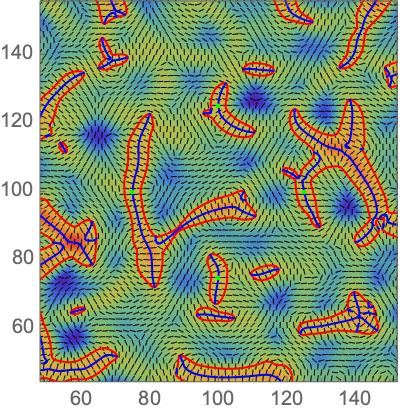
\includegraphics[width=\textwidth]{Composite_L}
\caption{$\lambda_1$, $\bm{v}_1$}
\end{subfigure}~
\begin{subfigure}[b]{0.49\textwidth}
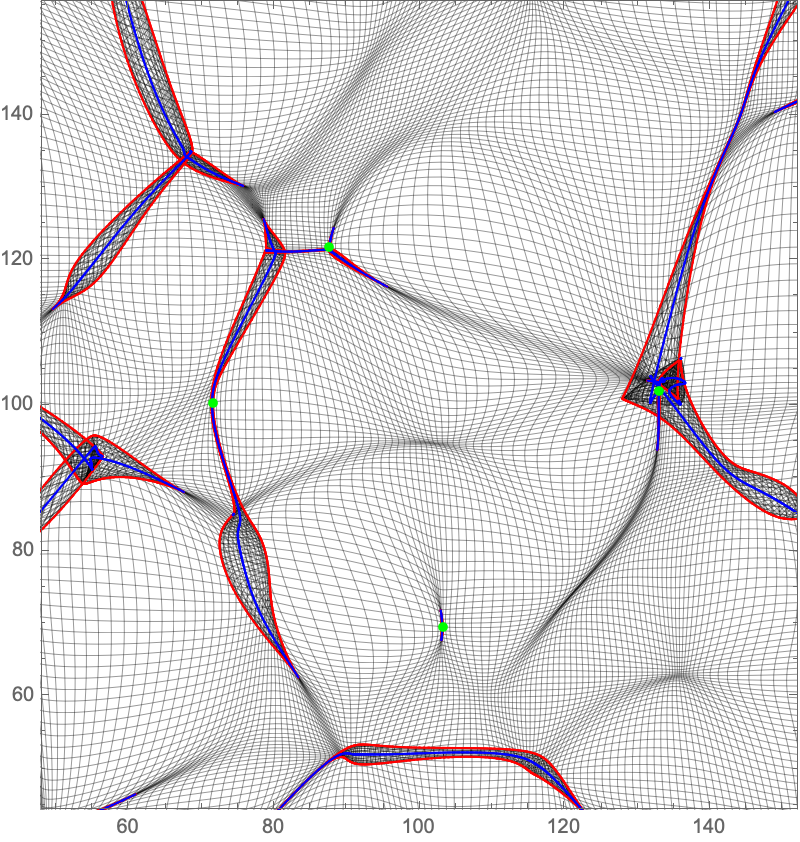
\includegraphics[width=\textwidth]{Composite_Z}
\caption{Zel'dovich approximation}
\end{subfigure}
\caption{Four critical point constraints on the first eigenvalue field. \textit{Left:} the first eigenvalue and eigenvector fields in Lagrangian space. \textit{Right:} the Zel'dovich approximation in Eulerian space.}\label{fig:composite}
\end{figure}

We illustrate this procedure in figure \ref{fig:composite}, which includes four Morse point constraints on the first eigenvalue field. A critical point $\bm{q}_c$ appearing at time $t$ satisfies the condition
\begin{align}
\nabla \lambda_1(\bm{q}_c) = 0\,,\\
\lambda_1(\bm{q}_c)=1/b_+(t)\,.
\end{align}
In the eigenvector frame, this condition reduces to the linear constraints
\begin{align}
1/b_+ = T_{11} \geq T_{22}\,, \quad  T_{12}=0\,,\quad T_{111}=T_{112}=0\,.
\end{align}
See appendix \ref{ap:eigenvalueRel} for a derivation. The critical point is either a maximum, minimum -- corresponding to the Morse point $A_3^+$ -- or a saddle point -- corresponding to the Morse point $A_3^-$. We can differentiate between the two cases by evaluating the sign of the determinant of the Hessian $\mathcal{H}\lambda_1$. In the eigenframe the Hessian takes the form
\begin{align}
\mathcal{H}\lambda_1 = 
\begin{pmatrix} 
T_{1111}+\frac{2T_{112}^2}{T_{11}-T_{22}} & T_{1112} + \frac{2 T_{112}T_{122}}{T_{11}-T_{22}} \\
T_{1112}+\frac{2 T_{112}T_{122}}{T_{11}-T_{22}} & T_{1122} + \frac{2 T_{122}^2}{T_{11}-T_{22}}
\end{pmatrix}\,.
\end{align}
See appendix \ref{ap:eigenvalueRel} for a derivation of this result. In figure \ref{fig:composite}, the lower, the upper, and the right critical points are $A_3^+$ points. The left critical point is a $A_3^-$ point. In the right panel we can clearly distinguish the character of the $A_3^+$ and $A_3^-$ points. The $A_3^+$ points correspond to the creation of a multi-stream region forming a Zel'dovich pancake. The $A_3^-$ points correspond to the merger of two multi-stream regions.


%%%%%%%%%%%%%%%%%%%%%%%%%%%%%%%%%%%%%%%%%%%%%%%%%%%%%%%%%%%%%%%%
\section{The caustic skeleton in Eulerian space}
To develop a visual appreciation of the roles of the different caustics in the large scale structure and the accuracy of the caustic skeleton of the Zel'dovich approximation, we construct a realization of an unconstrained Gaussian random field with the spectral index $n_s=-1$ and the smoothing scale $\sigma=2.5 \text{ Mpc}$ for the gravitational potential $\phi_0$ and evolve it with the Zel'dovich approximation and a small two-dimensional dark matter $N$-body simulation \cite{Hidding:2020} (see figure \ref{fig:Eulerian}) in a flat Einstein-de Sitter universe with the dark matter density $\Omega_m=1$ and Hubble constant $H_0=71\text{ Mpc/s/km}$. 

The caustic skeleton captures the geometry of the first eigenvalue and eigenvector field $\lambda_1$ and $\bm{v}_1$ (see the upper left panel). At late times, the cusp curves form an interconnected network tracing multi-stream regions bounded by the fold curves. The blue regions bounded by the fold curves are the progentors of the voids. At large scales, the eigenvalue field closely resembles the initial density perturbation $\delta_0 \propto \nabla^2\phi_0$ (see the upper right panel). Moreover, at these scales, the caustic skeleton follows the geometry of the superlevel sets of the density perturbation. However, on small scales, we observe qualitative differences. 

The Zel'dovich approximation clearly fails for late times. The approximation linearly extrapolates the initial flow of the mass elements, ignores any further change in the gravitational interactions and overshoots after shell-crossing (see the lower left panel of figure \ref{fig:Eulerian}). However, even though the Zel'dovich approximation no-longer accurately predicts the location of the multi-stream regions and the density field, it does predict the locations and times at which mass elements undergo shell-crossing and form caustics in Lagrangian space at these late times (see the lower right panel). The fold curves provide an reasonable approximation of the boundaries of the multi-stream regions. The cusp curves neatly bisect the multi-stream regions and form knots in the clusters of the cosmic web. Note that a cluster rarely consists of a single cluster caustics. Caustic correlated and together form intricate multi-stream regions in the knots. The filaments evolve more linearly and can often be associated to an unique cusp curve.
\begin{figure}
\centering
\begin{subfigure}[b]{0.49\textwidth}
\includegraphics[width=\textwidth]{Eulerian_L}
\caption{$\lambda_1,\bm{v}_1$}
\end{subfigure}~
\begin{subfigure}[b]{0.49\textwidth}
\includegraphics[width=\textwidth]{Eulerian_dens}
\caption{$\delta$}
\end{subfigure}\\
\begin{subfigure}[b]{0.49\textwidth}
\includegraphics[width=\textwidth]{Eulerian_Z}
\caption{Zel'dovich approximation}
\end{subfigure}~
\begin{subfigure}[b]{0.49\textwidth}
\includegraphics[width=\textwidth]{Eulerian_Nb}
\caption{$N$-body simulation}
\end{subfigure}
\caption{The caustic skeleton. \textit{Upper left:} the initial eigenvalue field $\lambda_1$ with the caustic skeleton. \textit{Upper right:} the initial density perturbations with the caustic skeleton. \textit{Lower left:} the Zel'dovich approximation with the caustic skeleton at scale factor $a=1$. \textit{Lower right:} the $N$-body simulation with the caustic skeleton at scale factor $a=1$.}\label{fig:Eulerian}
\end{figure}

\begin{figure}
\centering
\begin{subfigure}[b]{0.49\textwidth}
\includegraphics[width=\textwidth]{Evolution_020}
\caption{$a=0.2$}
\end{subfigure}~
\begin{subfigure}[b]{0.49\textwidth}
\includegraphics[width=\textwidth]{Evolution_040}
\caption{$a=0.4$}
\end{subfigure}\\
\begin{subfigure}[b]{0.49\textwidth}
\includegraphics[width=\textwidth]{Evolution_060}
\caption{$a=0.6$}
\end{subfigure}~
\begin{subfigure}[b]{0.49\textwidth}
\includegraphics[width=\textwidth]{Evolution_080}
\caption{$a=0.8$}
\end{subfigure}
%\begin{subfigure}[b]{0.48\textwidth}
%\includegraphics[width=\textwidth]{Evolution_100}
%\end{subfigure}
\caption{The evolution of the caustic skeleton in an $N$-body simulation in an Einstein-de Sitter universe. The skeleton for scale factor $a=1$ can be seen in the lower right panel of figure \ref{fig:Eulerian}.}\label{fig:Eulerian_Evolution}
\end{figure}

The multi-stream regions of the cosmic web forms gradually. Its evolution is neatly captured by the dynamics of the caustic skeleton (see figure \ref{fig:Eulerian_Evolution}). At early times, the dark-matter sheet consisted of a single single-stream region. As the mass elements undergo gravitational collapse, we observe the formation of several Zel'dovich pancakes corresponding to the maxima of the eigenvalue field $\lambda_1$ (see the upper left panel). These multi-stream regions grow and connect at the saddle points of the eigenvalue fields to form the web-like structure we observe in redshift surveys (see the upper right and lower panels). Note that viralized filaments move coherently while the large voids expand and the smaller voids contract. In this process several filaments may  merge to form more massive structures.



%%%%%%%%%%%%%%%%%%%%%%%%%%%%%%%%%%%%%%%%%%%%%%%%%%%%%%%%%%%%%%%%
\section{Conclusion and Discussion}
In this paper, we have:
\begin{itemize}
\item extended constrained Gaussian random field theory to include non-linear constraints,
\item implemented the constrained conditions of the caustic skeleton in 2D,
\item illustrated the relevance of eigenvalue and eigenvector fields in large-scale structure formation.
\end{itemize}
In an upcomming paper, we will:
\begin{itemize}
\item extend these studies to the three-dimensional cosmic web,
\item study the constrained inintial conditions of the three-dimensional cosmic skeleton,
\item study the mean fields as a function of the formation time,
\item evaluate the eigenvalue fields and the derivatives in the eigenframes,
\item use the constrained initial conditions to study the mean density field around the different elements.
\end{itemize}


%%%%%%%%%%%%%%%%%%%%%%%%%%%%%%%%%%%%%%%%%%%%%%%%%%%%%%%%%%%%%%%%
\section*{Acknowledgement}
JF would like to thank Nynke Niezink for the enlightening discussions.


%%%%%%%%%%%%%%%%%%%%%%%%%%%%%%%%%%%%%%%%%%%%%%%%%%%%%%%%%%%%%%%%

%\bibliographystyle{JHEP}
\bibliographystyle{plain}

\bibliography{mybibliography}

\appendix
%%%%%%%%%%%%%%%%%%%%%%%%%%%%%%%%%%%%%%%%%%%%%%%%%%%%%%%%%%%%%%%%
\section{Gaussian random fields algorithms}\label{ap:GRF}
Gaussian random fields are most naturally expressed in Fourier space, as the Fourier modes of an unconstrained Gaussian random field are normally and independently distributed, 
\begin{align}
p(\hat{f}(\bm{k}_1), \hat{f}(\bm{k}_2), \dots) = \prod_{i} \frac{1}{\sqrt{2\pi P(\| \bm{k}_i\|)}} e^{-\frac{|\hat{f}(\bm{k}_i)|^2}{2P(\|\bm{k}_i\|)}},
\end{align}
up to the reality condition, $\hat{f}(\bm{k})=\hat{f}^*(-\bm{k})$. In this paper, we use Fast Fourier Transform routines to efficiently generate realizations of both unconstrained and linearly constrained Gaussian random.

%%%%%%%%%%%%%%%%%%%%%%%%%%%%%%%%%%%%%%%%%%%%%%%%%%%%%%%%%%%%%%%%
\subsection{Unconstrained Gaussian random fields}
We can efficiently generate realizations of an unconstrained Gaussian random fields on a rectangular lattice using Fast Fourier Transform routines. The Fourier modes of an isotropic and homogeneous Gaussian random field are independent distributed Gaussian variables with zero mean, $\mu=0$, and the standard deviation $\sigma = \sqrt{P(\|\bm{k}\|)}$. Using this observation we generate the realization by multiplying the Fourier transform of white noise with the square root of the power spectrum:\\

\begin{algorithm}[H]
\SetAlgoLined
\begin{enumerate}[itemsep=1ex, leftmargin=0cm, rightmargin=1cm]
\item Generate a realization of white noise $n_w(\bm{q})$, consisting of identically independently distributed normal numbers $\mathcal{N}(\mu=0,\sigma^2=1)$ on a regular rectangular lattice.
\item Fast Fourier transform the white noise $\hat{n}_w(\bm{k}) = \text{FFT}[n_w(\bm{q})]$. The Fourier modes are independently normally distributed satisfying the reality condition $\hat{n}_w(\bm{k}) = \hat{n}_w^*(-\bm{k})$.
\item Rescale the Fourier modes with the power spectrum $\hat{f}(\bm{k}) = \sqrt{P(\bm{k})}\hat{n}_w(\bm{k})$.
\item Evaluate the inverse fast Fourier transform the rescaled modes to obtain the realization of the unconstrained Gaussian random field $f(\bm{q}) = \text{FFT}^{-1}[\hat{f}(\bm{k})]$.
\end{enumerate}
 \caption{Generating a realization of an unconstrained Gaussian random field on a rectangular lattice}
 \label{alg:GRF}
\end{algorithm}$ $\\

%%%%%%%%%%%%%%%%%%%%%%%%%%%%%%%%%%%%%%%%%%%%%%%%%%%%%%%%%%%%%%%%
\subsection{Linearly constrained Gaussian random fields}
We efficiently generate realizations of constrained Gaussian random fields, satisfying a set of linear constraints $\Gamma=\{\bm{C}[f]=\bm{c}\}$, using the Hoffman Ribak algorithm \cite{Hoffman:1991, Weygaert:1996}. The algorithm is based on the observation that the residue of the random field with respect to the mean field, $\delta f = f - \langle f | \Gamma\rangle$, is a Gaussian random field whose properties are independent of the constraint values $\bm{c}$. Note that this is a special property of Gaussianity of the random field and the linearity of the constraints $\bm{C}$.

Given a free function $f$, we compute the value of the linear constraint $C_i$ using the convolution theorem
\begin{align}
C_i[f,\bm{q}_i]=\text{FFT}^{-1}[\hat{C}_i^*(\bm{k}) \hat{f}(\bm{k})](\bm{0})
\end{align}
evaluated at the origin, with the Fourier transform of the constraint $\hat{C}_i$. Assuming that the unconstrained mean field vanishes, $\langle f \rangle =0$, we evaluate the constrained mean field using the formula
\begin{align}
\langle f(\bm{q}) | \Gamma\rangle = \sum_{i,j} \xi_i(\bm{q})\xi_{ij}^{-1} c_j\,,
\end{align}
with the covariance between the random field and the constraint
\begin{align}
\xi_i(\bm{q}) = \text{FFT}^{-1}[\hat{C}_i(\bm{k}) P(\|\bm{k}\|)]\,,
\end{align}
and the covariance matrix of the constraints
\begin{align}
\xi_{ij}=\text{FFT}^{-1}[\hat{C}_i^*(\bm{k}) \hat{C}_i(\bm{k}) P(\|\bm{k}\|)](\bm{0})\,,
\end{align}
evaluated at the origin. In these equations, we assume that $\bar{f}=\bar{C}_i=0$. Note that the vector $\bm{\xi}(\bm{q})=[\sum_i \xi_i(\bm{q}) \xi_{ij}^{-1}]$ is a normal basis of the constraints. The mean field is the inner product of $\bm{x}$ with the constraint values, 
\begin{align}
\langle f(\bm{q}) | \Gamma\rangle = \bm{\xi}(\bm{q})\cdot \bm{c}\,.
\end{align}
We use these routines to implement the Hoffman-Ribak method:\\

\begin{algorithm}[H]
\SetAlgoLined
\begin{enumerate}[itemsep=1ex, leftmargin=0cm, rightmargin=1cm]
\item Generate a realization of an unconstrained Gaussian random field $g$ with the required power spectrum using algorithm \ref{alg:GRF}.
\item Evaluate the linear constraints $C_i$ of the unconstrained field $g$,
\begin{align}
d_i = C_i[g;\bm{q}_i]\,.
\end{align} 
\item Evaluate the mean field corresponding to the constraint values $d_i$,
\begin{align}
\bar{g}(\bm{q}) = \sum_{ij}\xi_i(\bm{q}) \xi^{-1}_{ij} d_j\,.
\end{align}
\item Evaluate the residue of the unconstrained field 
\begin{align}
\delta g=g - \bar{g}\,.
\end{align}
\item Since the residue $\delta g$ is statistically independent of the values $d_j$, we can identify $\delta g$ with the residue $\delta f$ of the constrained random field. The realization of the constrained Gaussian random field takes the form
\begin{align}
f(\bm{q}) = \sum_{ij}\xi_i(\bm{q}) \xi^{-1}_{ij} c_j + \delta g(\bm{q})\,.
\end{align}
\end{enumerate}
 \caption{The Hoffman-Ribak method for Gaussian random fields with linear constraints}
 \label{alg:HoffmanRibak}
\end{algorithm}


%%%%%%%%%%%%%%%%%%%%%%%%%%%%%%%%%%%%%%%%%%%%%%%%%%%%%%%%%%%%%%%%
\section{Constraint probability density}\label{ap:constraintDensity}
The conditional density 
\begin{align}
p(f|\Gamma) =\frac{p(f, \Gamma)}{p(\Gamma)}
\end{align}
with $\Gamma = \{\bm{C} = \bm{c}\}$ is a Gaussian density as both $p(f,\Gamma)$ and $p(\Gamma)$ are normally distributed. It thus suffices to evaluate the mean and covariance matrix. For completeness, we write the mean of the function and the constraints as $\bar{f}(\bm{q})=\langle f(\bm{q}) \rangle$ and $\bar{\bm{C}}=\langle \bm{C}\rangle$, and the covariance as
\begin{align}
\xi(\bm{q}_1,\bm{q}_2)& = \text{cov}(f(\bm{q}_1),f(\bm{q}_2))= \langle (f(\bm{q}_1) - \bar{f}(\bm{q}_1))(f(\bm{q}_2) - \bar{f}(\bm{q}_2))\rangle\,,\\
\xi_i(\bm{q}) &= \text{cov}(f(\bm{q}),C_i) = \langle (f(\bm{q})-\bar{f}(\bm{q}))(C_i - \bar{C}_i)\rangle\,,\\
\xi_{ij} &= \text{cov}(C_i,C_j) = \langle (C_i - \bar{C}_i)(C_j-\bar{C}_j)\rangle\,.
\end{align}
For conciseness, we use the Einstein summation convention over the repeated dummy indices.

Define an auxiliary function $g(\bm{q}) = f(\bm{q}) + \bm{A}(\bm{q}) \cdot \bm{C}$ with $A_i(\bm{q}) = -\xi_j(\bm{q}) \xi_{ji}^{-1}$. The function $g$ is by construction independent of the variable $\bm{C}$, as they are jointly normally distributed and their covariance matrix vanishes, \textit{i.e.}, 
\begin{align}
\text{cov}(g(\bm{q}),\bm{C})
&=\text{cov}(f(\bm{q}),\bm{C}) +  \text{cov}(\bm{C},\bm{C}) \bm{A}(\bm{q}) \\
&=[\xi_k(\bm{q}) - \xi_i(\bm{q}) \xi_{ij}^{-1}\xi_{jk}]_{k=1}^N\\
&=\bm{0}\,.
\end{align}
The expectation value of $g$ is $\langle g(\bm{q})\rangle = \bar{f}(\bm{q}) + \bm{A}(\bm{q}) \cdot \bar{\bm{C}}$, which we can use to evaluate the expectation value of the constrained field
\begin{align}
\langle f(\bm{q}) | \Gamma \rangle 
&=\langle g(\bm{q}) - \bm{A}(\bm{q})\cdot \bm{C}|\Gamma\rangle\\
&=\langle g(\bm{q})\rangle - \bm{A}(\bm{q}) \cdot \bm{c}\\
&=\bar{f}(\bm{q}) + \bm{A}(\bm{q})\cdot (\bar{\bm{C}}-\bm{c})\\
&= \bar{f}(\bm{q}) + \xi_i(\bm{q})\xi_{ij}^{-1}(c_j -\bar{C}_j)\,.
\end{align}
When $\bar{f} = 0$ and $\bar{\bm{C}}=\bm{0}$ the expectation value reduces to the identity $\langle f(\bm{q}) | \Gamma \rangle =\xi_i(\bm{q})\xi_{ij}^{-1}c_j$. The covariance of the constraint field follows along similar lines
%\begin{align}
%\text{var}(f(\bm{q})|\Gamma) 
%&= \text{var}(g(\bm{q}) - \bm{A}(\bm{q})\cdot \bm{C}|\Gamma) \\
%&= \text{var}(g(\bm{q})|\Gamma) + \text{var}(\bm{A}(\bm{q})\cdot \bm{C}|\Gamma) -2 \bm{A}(\bm{q})\cdot \text{cov}(g(\bm{q}), \bm{C}|\Gamma)\\
%&= \text{var}(g(\bm{q})) \\
%&=\text{var}(f(\bm{q}) + \bm{A}(\bm{q})\cdot \bm{C})\\
%&=\text{var}(f(\bm{q})) + \bm{A}^T(\bm{q}) \text{var}(\bm{C}) \bm{A}(\bm{q}) + 2\bm{A}(\bm{q}) \cdot \text{cov}(f(\bm{q}),\bm{C}) \\
%&=\text{var}(f(\bm{q})) + \xi_i(\bm{q})\xi_{ij}^{-1}\xi_{jk}\xi_{kl}^{-1}\xi_{l}(\bm{q}) - 2\xi_i(\bm{q})\xi_{ij}^{-1}\xi_{j}(\bm{q})\\
%&=\xi(\bm{0}) - \xi_i(\bm{q}) \xi_{ij}^{-1} \xi_j(\bm{q})\,.
%\end{align}
\begin{align}
\text{cov}(f(\bm{q}_1), f(\bm{q}_2)|\Gamma) 
&= \text{cov}(g(\bm{q}_1) - \bm{A}(\bm{q}_1)\cdot \bm{C}, g(\bm{q}_2) - \bm{A}(\bm{q}_2)\cdot \bm{C}|\Gamma) \\
&= \text{cov}(g(\bm{q}_1), g(\bm{q}_2)|\Gamma) + \text{cov}(\bm{A}(\bm{q}_1)\cdot \bm{C}, \bm{A}(\bm{q}_2)\cdot \bm{C}|\Gamma)\\
&\ \ \  - \bm{A}(\bm{q}_1)\cdot \text{cov}(\bm{C}, g(\bm{q}_2)|\Gamma) -\text{cov}(g(\bm{q}_1) , \bm{C}|\Gamma)\cdot \bm{A}(\bm{q}_2)\\
&= \text{cov}(g(\bm{q}_1), g(\bm{q}_2)) \\
&=\text{cov}(f(\bm{q}_1) + \bm{A}(\bm{q}_1)\cdot \bm{C}, f(\bm{q}_2) + \bm{A}(\bm{q}_2)\cdot \bm{C})\\
&=\text{cov}(f(\bm{q}_1), f(\bm{q}_2)) + \bm{A}(\bm{q}_1) \text{cov}(\bm{C},\bm{C}) \bm{A}^T(\bm{q}_2) \\
&\ \ \ + \bm{A}(\bm{q}_1) \cdot \text{cov}(\bm{C},f(\bm{q}_2))+ \text{cov}(f(\bm{q}_1), \bm{C}) \cdot \bm{A}(\bm{q}_2) \\
&=\text{cov}(f(\bm{q}_1), f(\bm{q}_2)) + \xi_i(\bm{q}_1)\xi_{ij}^{-1}\xi_{jk}\xi_{kl}^{-1}\xi_{l}(\bm{q}_2) - 2\xi_i(\bm{q}_1)\xi_{ij}^{-1}\xi_{j}(\bm{q}_2)\\
&=\xi(\bm{q}_1,\bm{q}_2) - \xi_i(\bm{q}_1) \xi_{ij}^{-1} \xi_j(\bm{q}_2)\,.
\end{align}
We conclude that the residue $\delta f$ of $f$ with respect to the mean field $\langle f(\bm{q})|\Gamma\rangle =\bar{f}(\bm{q})+ \xi_i(\bm{q})\xi_{ij}^{-1}(c_j-\bar{C}_j)$ is a Gaussian random field with zero mean $\langle \delta f|\Gamma\rangle=0$ and variance $\langle \delta f(\bm{q})^2|\Gamma\rangle = \sigma_0^2 - \xi_i(\bm{q}) \xi_{ij}^{-1} \xi_j(\bm{q})$. Note that the residue $\delta f$ for a Gaussian random field with linear constraints is indeed independent of $\bm{c}$. The covariance of the constraint field yields the constrained probability density
\begin{align}
p(f|\Gamma) \propto  e^{-\frac{1}{2} \iint \delta{f}(\bm{q}_1) \tilde{K}(\bm{q}_1,\bm{q}_2) \delta f(\bm{q}_2)\mathrm{d}\bm{q}_1 \mathrm{d}\bm{q}_2 }\label{eq:constraint2}
\end{align}
with the residue $\delta f = f-\bar{f}(\bm{q})+ \xi_i(\bm{q})\xi_{ij}^{-1}(c_j-\bar{C}_j)$ and the kernel $\tilde{K}$ defined as the inverse of the modified two point correlation function, \textit{i.e.},
\begin{align}
\int \tilde{K}(\bm{q}_1,\bm{q}) \left[\xi(\bm{q},\bm{q}_2) - \xi_i(\bm{q})\xi_{ij}^{-1}\xi_j(\bm{q}_2)\right]\mathrm{d}\bm{q}= \delta_D^{(2)}(\bm{q}_1-\bm{q}_2)\,.
\end{align}
The correction $- \xi_i(\bm{q})\xi_{ij}^{-1}\xi_j(\bm{q}_2)$ implements the statistical anisotropy and inhomogeneity of the residue.


%%%%%%%%%%%%%%%%%%%%%%%%%%%%%%%%%%%%%%%%%%%%%%%%%%%%%%%%%%%%%%%%
\section{Non-linear eigenvalue relations}\label{ap:eigenvalueRel}
The eigenvalue and eigenvector fields are non-linear functions of the deformation tensor
\begin{align}
\bm{\psi} = \begin{pmatrix} T_{11} & T_{12} \\ T_{12} & T_{22}\end{pmatrix},
\end{align}
with the partial derivatives of the displacement potential $T_{ijk\dots} = \frac{\partial}{\partial q_i}\frac{\partial}{\partial q_j}\frac{\partial}{\partial q_k}\dots \Psi$. In two dimensions, the eigenvalue and eigenvector fields are the quadratic roots of the eigenequation $\bm{\psi}\bm{v}_i=\lambda_i \bm{v}_i$, with the explicit identities for the eigenvalue fields
\begin{align}
\lambda_1(T_{11},T_{22},T_{12}) &= \frac{1}{2}\left(T_{11}+T_{22} + \sqrt{4 T_{12}^2 +(T_{11}-T_{22})^2}\right)\,,\\
\lambda_2(T_{11},T_{22},T_{12}) &= \frac{1}{2}\left(T_{11}+T_{22} - \sqrt{4 T_{12}^2 +(T_{11}-T_{22})^2}\right)\,.
\end{align}
To study Gaussian random fields satisfying non-linear constraints in terms of the eigenvalue and eigenvector fields, it is convenient to develop several identities in the eigenframe, for which $T_{11} \geq T_{22}$ and $T_{12}=0$. Note that in this frame the eigenvalue and eigenvector fields locally take the form
\begin{align}
\lambda_{1} &= T_{11}\,,\quad \bm{v}_1=(1,0)\,,\\
\lambda_{2} &= T_{22}\,,\quad \bm{v}_2=(0,1)\,.
\end{align}

The eigenvalue decomposition $\bm{\psi} = R^T \Lambda R,$ with the the diagonal matrix
\begin{align}
\Lambda = \begin{pmatrix}\lambda_1 & 0 \\ 0 &\lambda_2 \end{pmatrix}
\end{align}
satisfying the ordering $\lambda_1 \geq \lambda_2$, and the rotation matrix
\begin{align}
R = \begin{pmatrix} \cos \theta & - \sin \theta \\ \sin \theta & \cos \theta \end{pmatrix} \in SO(2),
\end{align}
yield three identies for the components of the deformation tensor $T_{11},T_{22},T_{12}$ 
\begin{align}
T_{11} &= \lambda_1 \cos^2 \theta + \lambda_2 \sin^2 \theta\,,\\
T_{22} &= \lambda_1 \sin^2\theta + \lambda_2 \cos^2 \theta\,,\\
T_{12} &= (\lambda_2 - \lambda_1)\cos \theta \sin \theta\,.
\end{align}
Solving for the angle $\theta$, we obtain a representation for the normalized eigenvector fields
\begin{align}
\bm{v}_1 &=\pm (\cos(\theta), -\sin(\theta))\,,\\
\bm{v}_2 &=\pm (\sin(\theta),\ \ \ \cos(\theta))\,,
\end{align}
where the sine and cosine are expressed in terms of the partial derivatives of the displacement potential
\begin{align}
\cos(\theta) &= \frac{\sqrt{T_{11} - T_{22} + \sqrt{4 T_{12}^2 +(T_{11}-T_{22})^2}}}{\sqrt{2} \sqrt[4]{4T_{12}^2 + (T_{11}-T_{22})^2}}\,,\\
\sin(\theta) &= \frac{\sqrt{2}T_{12}}{\sqrt[4]{4T_{12}^2+(T_{11}-T_{22})^2}\sqrt{T_{11}-T_{22} + \sqrt{4T_{12}^2 + (T_{11}-T_{22})^2}}}\,.
\end{align}
These relations enable us to evaluate several useful non-linear identities. We evaluate the derivatives of the eigenvalue field in a general frame and subsequently take the limit $T_{12} \to 0$ with the condition $T_{11}\geq T_{22}$. 

The first order derivatives of the eigenvalue fields in the eigenframe take are linear 
\begin{align}
\frac{\partial}{\partial q_1} \lambda_1&= T_{111}\,,\quad
\frac{\partial}{\partial q_2} \lambda_1= T_{112}\,,\\
\frac{\partial}{\partial q_1} \lambda_2&= T_{122}\,,\quad
\frac{\partial}{\partial q_2} \lambda_2= T_{222}\,.
\end{align}
The second order derivatives receive a non-linear correction
\begin{align}
\frac{\partial^2}{\partial q_1^2} \lambda_1&= T_{1111} + \frac{2 T_{112}^2}{T_{11}-T_{22}}\,,\\
\frac{\partial^2}{\partial q_1 \partial q_2} \lambda_1&= T_{1112} + \frac{2 T_{112}T_{122}}{T_{11}-T_{22}}\,,\\
\frac{\partial^2}{\partial q_2^2} \lambda_1&= T_{1122} + \frac{2T_{122}^2}{T_{11}-T_{22}}\,,\\
\frac{\partial^2}{\partial q_1^2} \lambda_2&= T_{1122} - \frac{2 T_{112}^2}{T_{11}-T_{22}}\,,\\
\frac{\partial^2}{\partial q_1 \partial q_2} \lambda_2&= T_{1222} - \frac{2 T_{112}T_{122}}{T_{11}-T_{22}}\,,\\
\frac{\partial^2}{\partial q_2^2} \lambda_2&= T_{2222} - \frac{2T_{122}^2}{T_{11}-T_{22}}\,.
\end{align}

The first order derivative in the direction of the eigenvalue field naturally coincide with the first order derivatives described above
\begin{align}
\bm{v}_1 \cdot \nabla \lambda_1 &= \pm T_{111}\,,\quad
\bm{v}_2 \cdot \nabla \lambda_1 = \pm T_{112}\,,\\
\bm{v}_1 \cdot \nabla \lambda_2 &= \pm T_{122}\,,\quad
\bm{v}_2 \cdot \nabla \lambda_2 = \pm T_{222}\,.
\end{align}
Note that these combinations transform as scalars under rotations. The second order derivatives receive an additional non-linear term due to the variation of the eigenvector fields. The second order derivatives of the first eigenvalue field take the form
\begin{align}
\bm{v}_1 \cdot \nabla (\bm{v}_1 \cdot \nabla \lambda_1) &= T_{1111} + \frac{3T_{112}^2}{T_{11}-T_{22}}\,,\\
\bm{v}_2 \cdot \nabla (\bm{v}_1 \cdot \nabla \lambda_1) &= \pm \left[T_{1112} + \frac{3T_{112}T_{122}}{T_{11}-T_{22}}\right]\,,\\
\bm{v}_1 \cdot \nabla (\bm{v}_2 \cdot \nabla \lambda_1) &= \pm \left[T_{1112} - \frac{T_{112}(T_{111}-2T_{122})}{T_{11}-T_{22}}\right]\,,\\
\bm{v}_2 \cdot \nabla (\bm{v}_2 \cdot \nabla \lambda_1) &= T_{1122} - \frac{T_{122}(T_{111}-2T_{122})}{T_{11}-T_{22}}\,.
\end{align}
Note that the directional derivatives in the directions $\bm{v}_1$ and $\bm{v}_2$ do not commute. The second order derivatives of the second eigenvalue field yield the analogous identities
\begin{align}
\bm{v}_1 \cdot \nabla (\bm{v}_1 \cdot \nabla \lambda_2) &= T_{1122} + \frac{T_{112}(T_{222}-2T_{112})}{T_{11}-T_{22}}\,,\\
\bm{v}_2 \cdot \nabla (\bm{v}_1 \cdot \nabla \lambda_2) &= \pm\left[T_{1222} + \frac{T_{122}(T_{222}-2T_{112})}{T_{11}-T_{22}}\right]\,,\\
\bm{v}_1 \cdot \nabla (\bm{v}_2 \cdot \nabla \lambda_2) &= \pm\left[T_{1222} - \frac{3T_{112}T_{122}}{T_{11}-T_{22}}\right]\,,\\
\bm{v}_2 \cdot \nabla (\bm{v}_2 \cdot \nabla \lambda_2) &= T_{2222} - \frac{3T_{122}^2}{T_{11}-T_{22}}\,.
\end{align}


%%%%%%%%%%%%%%%%%%%%%%%%%%%%%%%%%%%%%%%%%%%%%%%%%%%%%%%%%%%%%%%%
\section{Rotations of derivatives of the deformation tensor}\label{ap:rotations}
Under a rotation, the derivatives of the deformation tensor transform nontrivailly. When applying the rotation matrix
\begin{align}
R_\theta = \begin{pmatrix} c  & s  \\- s  & c \end{pmatrix},
\end{align}
with $c=\cos\theta$ and $s=\sin \theta$, the first, second, third, and fourth order derivatives transform into each other. The first order derivatives transform as a vector
\begin{align}
\begin{pmatrix} T_1 \\ T_2 \end{pmatrix}
\mapsto
\begin{pmatrix}
c & -s \\
s &  c 
\end{pmatrix}
\begin{pmatrix} T_1 \\ T_2 \end{pmatrix}.
\end{align}
The second order derivatives transform as
\begin{align}
\begin{pmatrix} T_{11} \\ T_{12} \\ T_{22} \end{pmatrix}
\mapsto
\begin{pmatrix}
c^2 & -2 c s    &  s^2 \\
c s &  c^2- s^2 & -c s \\
s^2 & 2c s      &  c^2 
\end{pmatrix}
\begin{pmatrix} T_{11} \\ T_{12} \\ T_{22} \end{pmatrix}.
\end{align}
The third order derivatives transform as
\begin{align}
\begin{pmatrix} T_{111} \\ T_{112} \\ T_{122}\\ T_{222} \end{pmatrix}
\mapsto
\begin{pmatrix}
c^3   & -3 c^2 s        & 3 c s^2          & -s^3   \\
c^2 s &  c(c^2 - 2 s^2) & s( s^2- 2 c^2)   &  c s^2 \\
c s^2 &  s(2 c^2 - s^2) & c(c^2 -  2 s^2)  & -c^2 s \\
s^3   &  3 c s^2        & 3 c^2 s          & c^3 
\end{pmatrix}
\begin{pmatrix} T_{111} \\ T_{112} \\ T_{122}\\ T_{222} \end{pmatrix}.
\end{align}
The fourth order derivatives transform as
\begin{align}
\begin{pmatrix} T_{1111} \\ T_{1112} \\ T_{1122}\\ T_{1222} \\ T_{2222} \end{pmatrix}
\mapsto
\begin{pmatrix}
c^4     & -4 c^3 s          & 6 c^2 s^2               &- 4 c s^3          &  s^4     \\
c^3 s   & c^2(c^2 - 3 s^2)  & 3cs(s^2 - c^2)     & s^2(3 c^2  - s^2) & -c s^3   \\
c^2 s^2 & 2cs( c^2 -  s^2)  & c^4  - 4 c^2 s^2  + s^4 & 2cs(  s^2 -  c^2) &  c^2 s^2 \\
c s^3   & s^2(3 c^2  - s^2) & 3cs( c^2 - s^2 )   & c^2(c^2  - 3 s^2) & -c^3 s   \\
s^4     & 4cs^3             & 6 c^2 s^2               & 4 c^3 s           &  c^4 
\end{pmatrix}
\begin{pmatrix} T_{1111} \\ T_{1112} \\ T_{1122}\\ T_{1222} \\ T_{2222} \end{pmatrix}.
\end{align}



\newpage
%%%%%%%%%%%%%%%%%%%%%%%%%%%%%%%%%%%%%%%%%%%%%%%%%%%%%%%%%%%%%%%%
\section{Notes}
The derivation of the non-linear eigenvalue relations does not straigforwardly generalize to the three dimensional case. However, using algabra we can do it anyway. We first rederive the identities obtained in appendix \ref{ap:eigenvalueRel}. We subsequently generalize these relations to 3D.

In two dimensions, we have the identities
\begin{align}
\text{Tr}\ \bm{\psi} &= T_{11} + T_{22} = \lambda_1 + \lambda_2\\
\text{det}\ \bm{\psi} &=  T_{11}  T_{22} - T_{12}^2 = \lambda_1 \lambda_2
\end{align}
Assuming $T_{11} \geq T_{22}$, these equations have a unique solution. In the eigenframe $T_{12}=0$, we obtain $\lambda_1 = T_{11}$ and $\lambda_2=T_{22}$, and we will assume $\bm{v}_1=(1,0)$ and $\bm{v}_2=(0,1)$. Next, apply the differential operators $\partial_i$ and $\partial_{i}\partial_j$ for $i,j=1,2$, leading to a set of four identities. Rotate to the eigenframe by substituting $\lambda_1 = T_{11}$, $\lambda_2=T_{22}$, and $T_{12}=0$. If we now solve for $\partial_i\lambda_j$ and $\partial_i \partial_j \lambda_k$, we obtain the first set of non-linear eigen identities.

To study the directional derivatives in the direction of the eigenvectors, we use the chain rule 
\begin{align}
\bm{v}_i \cdot \nabla (\bm{v}_j \cdot \nabla \lambda_k)= (\bm{v}_i \cdot  \nabla )\bm{v}_j \cdot \nabla \lambda_k + \bm{v}_i (\mathcal{H} \lambda_k )\bm{v}_j \,,
\end{align}
with the Hessian $\mathcal{H}$. We already obtained the rightmost term in the eigenframe from the analysis above. What remains is evaluating the derivative $(\bm{v}_i \cdot \nabla) \bm{v}_j$. First note that the normalization $\|\bm{v}_i\|=1$ implies the identity
\begin{align}
\bm{v}_i \cdot \partial_j \bm{v}_i=0\,.
\end{align} 
The vector $\partial_i \bm{v}_j$ is normal to $\bm{v}_j$ fixing one of the coefficients of $(\bm{v}_i \cdot \nabla) \bm{v}_j$. For the remaining coefficients, we use the eigenequation $(\bm{\psi}-\lambda_i I)\bm{v}_i=\bm{0}$. After applying the operator $\partial_j$, we obtain the relation
\begin{align}
(\partial_j \bm{\psi} - \partial_j \lambda_j I)\bm{v}_i + (\bm{\psi}-\lambda_i I)\partial_j \bm{v}_i=\bm{0}\,.
\end{align}
In the eigenframe, these equations are solved by
\begin{align}
\nabla \bm{v}_1 &= \begin{pmatrix}
0, & T_{112}/(T_{11}-T_{22})\\
0, & T_{122}/(T_{11}-T_{22})
\end{pmatrix},\\
\nabla \bm{v}_2 &= \begin{pmatrix}
-T_{112}/(T_{11}-T_{22}), & 0\\
-T_{122}/(T_{11}-T_{22}), & 0
\end{pmatrix}.
\end{align}
When combining all the terms we reproduce the results presented in appendix \ref{ap:eigenvalueRel}.


This calculation straigtforwardly extends to symmetric $3\times 3$ matrices. We start with the identities
\begin{align}
\text{Tr}\ \bm{\psi} &= \lambda_1 + \lambda_2 + \lambda_3\,,\\
\frac{1}{2}((\text{Tr}\ \bm{\psi})^2 - \text{Tr}\ \bm{\psi}^2) &= \lambda_1 \lambda_2 + \lambda_1 \lambda_3 + \lambda_2 \lambda_3\,,\\
\text{det}\ \bm{\psi} &= \lambda_1 \lambda_2 \lambda_3\,.
\end{align}
In the eigenframe, we have $\lambda_1=T_{11}, \lambda_2=T_{22},\lambda_3=T_{33}$ and $T_{12}=T_{13}=T_{23}=0$ assuming $T_{11} \geq T_{22} \geq T_{33}$ and $\bm{v}_1=(1,0,0)$, $\bm{v}_2=(0,1,0)$, and $\bm{v}_3=(0,0,1)$. Applying the operators $\partial_i$ and $\partial_i \partial_j$ for $i,j=1,2,3$ and solving for the partial derivatives of the eigenvalue fields, we obtain in the eigenframe
\begin{align}
\nabla \lambda_1 &=(T_{111},T_{112},T_{113})\,,\\
\nabla \lambda_2 &=(T_{122},T_{222},T_{223})\,,\\
\nabla \lambda_3 &=(T_{133},T_{233},T_{333})\,,
\end{align}
and for the first eigenvalue field
\begin{align}
\partial_1 \partial_1 \lambda_1 &= T_{1111} - \frac{2 \left(T_{11} T_{123}^2+T_{112}^2 T_{33}+T_{113}^2 T_{22}\right)}{(T_{11}-T_{22}) (T_{11}-T_{33})}\,,\\
\partial_1 \partial_2 \lambda_1 &= T_{1112} - \frac{2 (T_{11} T_{123} T_{223}+T_{112} T_{122} T_{33}+T_{113} T_{123} T_{22})}{(T_{11}-T_{22}) (T_{11}-T_{33})}\,, \\
\partial_1 \partial_3 \lambda_1 &= T_{1113} - \frac{2 (T_{11} T_{123} T_{233}+T_{112} T_{123} T_{33}+T_{113} T_{133} T_{22})}{(T_{11}-T_{22}) (T_{11}-T_{33})}\,, \\
\partial_2 \partial_2 \lambda_1 &= T_{1122} - \frac{2 \left(T_{11} T_{223}^2+T_{122}^2 T_{33}+T_{123}^2 T_{22}\right)}{(T_{11}-T_{22}) (T_{11}-T_{33})}\,, \\
\partial_2 \partial_3 \lambda_1 &= T_{1123} - \frac{2 (T_{11} T_{223} T_{233}+T_{122} T_{123} T_{33}+T_{123} T_{133} T_{22})}{(T_{11}-T_{22}) (T_{11}-T_{33})}\,, \\
\partial_3 \partial_3 \lambda_1 &= T_{1133} - \frac{2 \left(T_{11} T_{233}^2+T_{123}^2 T_{33}+T_{133}^2 T_{22}\right)}{(T_{11}-T_{22}) (T_{11}-T_{33})}\,, 
\end{align}
and for the second eigenvalue field
\begin{align}
\partial_1 \partial_1 \lambda_2 &= T_{1122} + \frac{2 \left(T_{11} T_{123}^2+T_{112}^2 T_{33}+T_{113}^2 T_{22}\right)}{(T_{11}-T_{22}) (T_{22}-T_{33})}\,,\\
\partial_1 \partial_2 \lambda_2 &= T_{1222} + \frac{2 (T_{11} T_{123} T_{223}+T_{112} T_{122} T_{33}+T_{113} T_{123} T_{22})}{(T_{11}-T_{22}) (T_{22}-T_{33})}\,,\\
\partial_1 \partial_3 \lambda_2 &= T_{1223} + \frac{2 (T_{11} T_{123} T_{233}+T_{112} T_{123} T_{33}+T_{113} T_{133} T_{22})}{(T_{11}-T_{22}) (T_{22}-T_{33})}\,,\\
\partial_2 \partial_2 \lambda_2 &= T_{2222} + \frac{2 \left(T_{11} T_{223}^2+T_{122}^2 T_{33}+T_{123}^2 T_{22}\right)}{(T_{11}-T_{22}) (T_{22}-T_{33})}\,,\\
\partial_2 \partial_3 \lambda_2 &= T_{2223} + \frac{2 (T_{11} T_{223} T_{233}+T_{122} T_{123} T_{33}+T_{123} T_{133} T_{22})}{(T_{11}-T_{22}) (T_{22}-T_{33})}\,,\\
\partial_3 \partial_3 \lambda_2 &= T_{2233} + \frac{2 \left(T_{11} T_{233}^2+T_{123}^2 T_{33}+T_{133}^2 T_{22}\right)}{(T_{11}-T_{22}) (T_{22}-T_{33})}\,, 
\end{align}
and for the thrid eigenvalue field
\begin{align}
\partial_1 \partial_1 \lambda_3 &= T_{1133} - \frac{2 \left(T_{11} T_{123}^2+T_{112}^2 T_{33}+T_{113}^2 T_{22}\right)}{(T_{11}-T_{33}) (T_{22}-T_{33})}\,,\\
\partial_1 \partial_2 \lambda_3 &= T_{1233} - \frac{2 (T_{11} T_{123} T_{223}+T_{112} T_{122} T_{33}+T_{113} T_{123} T_{22})}{(T_{11}-T_{33}) (T_{22}-T_{33})}\,,\\
\partial_1 \partial_3 \lambda_3 &= T_{1333} - \frac{2 (T_{11} T_{123} T_{233}+T_{112} T_{123} T_{33}+T_{113} T_{133} T_{22})}{(T_{11}-T_{33}) (T_{22}-T_{33})}\,,\\
\partial_2 \partial_2 \lambda_3 &= T_{2233} - \frac{2 \left(T_{11} T_{223}^2+T_{122}^2 T_{33}+T_{123}^2 T_{22}\right)}{(T_{11}-T_{33}) (T_{22}-T_{33})}\,,\\
\partial_2 \partial_3 \lambda_3 &= T_{2333} - \frac{2 (T_{11} T_{223} T_{233}+T_{122} T_{123} T_{33}+T_{123} T_{133} T_{22})}{(T_{11}-T_{33}) (T_{22}-T_{33})}\,,\\
\partial_3 \partial_3 \lambda_3 &= T_{3333} - \frac{2 \left(T_{11} T_{233}^2+T_{123}^2 T_{33}+T_{133}^2 T_{22}\right)}{(T_{11}-T_{33}) (T_{22}-T_{33})}\,.
\end{align}
The partial derivatives of the eigenvector fields in the eigenframe take the form

\begin{align}
\nabla  \bm{v}_1 &= \begin{pmatrix}
0, & T_{112}/(T_{11}-T_{22}), & T_{113}/(T_{11}-T_{33})\\
0, & T_{122}/(T_{11}-T_{22}), & T_{123}/(T_{11}-T_{33})\\
0, & T_{123}/(T_{11}-T_{22}), & T_{133}/(T_{11}-T_{33})
\end{pmatrix}\,,\\
\nabla \bm{v}_2 &= \begin{pmatrix}
-T_{112}/(T_{11}-T_{22}),& 0,& T_{123}/(T_{22}-T_{33})\\
-T_{122}/(T_{11}-T_{22}),& 0,& T_{223}/(T_{22}-T_{33})\\
-T_{123}/(T_{11}-T_{22}),& 0,& T_{233}/(T_{22}-T_{33})
\end{pmatrix}\,,\\
\nabla \bm{v}_3 &= \begin{pmatrix}
-T_{113}/(T_{11}-T_{33}), & -T_{123}/(T_{22}-T_{33}), & 0\\
-T_{123}/(T_{11}-T_{33}), & -T_{223}/(T_{22}-T_{33}), & 0\\
-T_{133}/(T_{11}-T_{33}), & -T_{233}/(T_{22}-T_{33}), & 0
\end{pmatrix}\,.
\end{align}
We can combine these to obtained the required identities for $\bm{v}_i \cdot \nabla (\bm{v}_j \cdot \nabla \lambda_k)$ in the eigenframe. Higher order derivatives follow analogously.


\end{document}
